\documentclass[10pt,journal,compsoc]{IEEEtran}
\usepackage{cite}
\usepackage{graphicx}
\usepackage{psfrag}
\usepackage{subfigure}
\usepackage{url}
\usepackage{color}
\usepackage{balance}
\usepackage[all]{xy}
\usepackage{listings}
\usepackage{array,booktabs,arydshln,xcolor}
\usepackage{tikz}
\usetikzlibrary{shapes,patterns,calc,shapes.geometric,arrows}
\usepackage{makecell}
\usepackage{multirow}
\usepackage{xcolor}
\usepackage{url}
\usepackage{amsthm}
\usepackage{pgfplots}
\usepackage{float}
\usepackage{amsmath}
\usepackage{soul}
\theoremstyle{definition}
\newtheorem{definition}{Definition}[section]
\newtheorem{example}{Example}[section]

% please place your own definitions here and don't use \def but
% \newcommand{}{}
\newcommand\CH[1]{\textcolor{blue}{{CHIARA - }{#1}}}
\newcommand\CL[1]{\textcolor{red}{{CLAUDIO - }{#1}}}
\newcommand\MC[1]{\textcolor{green}{{MARCO - }{#1}}}
\newcommand\AG[1]{\textcolor{orange}{{AG - }{#1}}}
\newcommand{\job}[1]{\ensuremath{J_{#1}}}
\newcommand{\trans}[1]{\ensuremath{T_{#1}}}
\newcommand{\coalition}[1]{\ensuremath{C_{#1}}}
\newcommand{\org}[1]{\ensuremath{o_{#1}}}
\newcommand{\Org}[1]{\ensuremath{O_{#1}}}
\newcommand{\s}[1]{\ensuremath{s_{#1}}}
\newcommand{\si}[1]{\ensuremath{s_{#1}}}
\newcommand{\sii}[1]{\ensuremath{s'_{#1}}}
\newcommand{\dataset}[1]{\ensuremath{D_{#1}}}
\newcommand{\origdataset}{\ensuremath{X}}
\newcommand{\transdataset}{\ensuremath{Y}}

\newcommand{\T}{\ensuremath{T}}
\newcommand{\TP}{\ensuremath{T^{P}}}
\newcommand{\TF}[1]{\ensuremath{T^F_{#1}}}
\newcommand{\tf}[1]{\ensuremath{t^f_{#1}}}
\newcommand{\tp}[1]{\ensuremath{t^p_{#1}}}

\newcommand{\G}{\ensuremath{G}}

\newcommand{\F}[1]{\ensuremath{F_{#1}}}

\newcommand{\plusOperator}{\ensuremath{\oplus}}
\newcommand{\timesOperator}{\ensuremath{\otimes}}

\newcommand{\V}{\ensuremath{V}}
\newcommand{\Vp}{\ensuremath{V'}}
\newcommand{\Vplus}{\ensuremath{V_{\plusOperator}}}
\newcommand{\Vtimes}{\ensuremath{V_{\timesOperator}}}
\newcommand{\Vpplus}{\ensuremath{V'_{\plusOperator}}}
\newcommand{\Vptimes}{\ensuremath{V'_{\timesOperator}}}


\newcommand{\vi}[1]{\ensuremath{v_{#1}}}
\newcommand{\vii}[1]{\ensuremath{v'_{#1}}}

\newcommand{\E}{\ensuremath{E}}

\newcommand{\myLambda}{\ensuremath{\lambda}\,}
\newcommand{\myGamma}{\ensuremath{\gamma}\,}
\newcommand{\templateChartAnnotation}{\ensuremath{\myLambda,\myGamma}}
\newcommand{\instanceChartAnnotation}{\ensuremath{\myLambda}}
\renewcommand{\P}[1]{\ensuremath{P_{#1}}}
\newcommand{\p}[1]{\ensuremath{p_{#1}}}
% \newcommand{\TF}{\ensuremath{T_{\fChartFunction}}}
\newcommand{\user}{user\,}
\newcommand{\User}{User\,}
\newcommand{\profile}{\emph{prf}}

\newcommand{\fChartFunction}{\ensuremath{\myLambda{}}}

\newcommand{\tChartFunction}{\ensuremath{G^{\myLambda,\myGamma}(\V,\E,\myLambda,\myGamma)}\xspace}
% \newcommand{\iChartFunction}{\ensuremath{\fChartFunction,\myGamma{},\myLambda{}}}
\newcommand{\iChartFunction}{\ensuremath{G'(\V',\E,\myLambda)}\xspace}
\newcommand{\windowsize}{\ensuremath{|w|}}
\newcommand{\bestcombination}{$G^*_w$}
\newcommand{\currentcombination}{$G'_w$}


\newcommand{\pipeline}{Pipeline\xspace}
\newcommand{\pipelineTemplate}{Pipeline Template\xspace}
\newcommand{\pipelineInstance}{Pipeline Instance\xspace}
\newcommand{\quality}{\textit{quality}\xspace}
\newcommand{\Quality}{\textit{Quality}\xspace}
\newcommand{\q}{\textit{Q}\xspace}
\newcommand{\pone}{$(service\_owner=dataset\_owner)$}
\newcommand{\ptwo}{$(service\_owner=partner(dataset\_owner))$}
\newcommand{\pthree}{$\langle service\_owner \neq dataset\_owner AND owner \neq partner(dataset\_owner)$}
% \newcommand{\function}{$\instanceChartAnnotation{}$}
% \newcommand{\function}{$\templateChartAnnotation$}
\newcommand{\average}{\textit{average}\xspace}
\newcommand{\wide}{\textit{wide}\xspace}
\newcommand{\problem}{Pipeline Instantiation Process }
\newcommand{\xmark}{\ding{55}}%
\newcommand{\cmark}{\ding{51}}%
\newcommand{\chia}[1]{{\color{red}#1}}
\newcommand{\policy}[5]{
  $\langle \text{#1},{#2},{#3},\ensuremath{#4},\ensuremath{#5} \rangle$
}





%\newcommand{\servicename}[1]{\emph{#1}\/}
\newcommand{\attrvalue}[1]{\emph{#1}\/}
\newcommand{\attrname}[1]{\emph{#1}\/}
\newcommand{\dimensionname}[1]{\emph{#1}\/}


%\newcommand{\cmshort}{\emph{CM}\/}
% certificate
%\newcommand{\cert}{Certificate}
% ct math
\newcommand{\mathct}{\ensuremath{\mathcal{M}}}
% cert math
\newcommand{\mathcert}{\ensuremath{\mathcal{C}}}
%
%
% new macro for categories
%
% dimension
%\newcommand{\mathdimensionname}[1]{\ensuremath{D_{#1}}}
%\newcommand{\mathdimension}[1]{\ensuremath{D_{#1}}}
\newcommand{\mathdimension}{\ensuremath{D}}
%\newcommand{\mathdimensioninstance}{\ensuremath{d}}

%
\newcommand{\mathproperty}{\ensuremath{p}}
\newcommand{\mathpropertyname}{\ensuremath{\hat{p}}}

% arguments are 1) dimension, 2) property
\newcommand{\mathlatticerel}{\ensuremath{\succeq}}
% need to provide the dimension including D, e.g., \mathlattice{D_{dev}}{conf}
\newcommand{\mathlattice}[2]{\ensuremath{(\mathcal{D}_{#1}, \mathlatticerel_{#2})}}
\newcommand{\mathdimlattice}{\ensuremath{\mathcal{D}}}
% need to provide only the subscript of D, e.g., \mathlatticedim{dev}{conf}
%\newcommand{\mathlatticedim}[2]{\ensuremath{(\mathcal{D}_{#1}, \mathlatticerel{#2})}}

\newcommand{\mathtarget}{\ensuremath{ToC}}

\newcommand{\mathattrvalue}{\ensuremath{v}}

\newcommand{\evid}{\ensuremath{ev}}
%\newcommand{\mathevidset}[1]{\ensuremath{EV_{#1}}}
\newcommand{\mathevidcollection}{\ensuremath{\mathcal{E}}}
%\newcommand{\mathevidcollectionset}[1]{\ensuremath{\mathcal{X}_{#1}}}
\newcommand{\mathevidsuccess}[1]{\ensuremath{\textit{Succ}(\evid_{#1})}}

% symbol to represent a mechanism
\newcommand{\mechanismsymbol}{\ensuremath{\theta}}
% symbol to represent a set of mechanisms
\newcommand{\mechanismsetsymbol}{\ensuremath{\Theta}}

% mechanism_ARG
\newcommand{\mathmechanism}[1]{\ensuremath{\mechanismsymbol_{#1}}}
% set of mechanism_ARG
\newcommand{\mathmechanismset}[1]{\ensuremath{\mechanismsetsymbol_{#1}}}
% binding functions between evidence and attributes
\newcommand{\mathbindingfn}{\ensuremath{\mathcal{B}}}
%\newcommand{\termbindingfn}{binding function}

%\newcommand{\termevid}{evidence}
%\newcommand{\termevidemph}{\emph{Evidence}}
%\newcommand{\termevidcollectm}{Evidence Collection Model}
%\newcommand{\termevidcollectmemph}{\emph{Evidence Collection Model}}

\newcommand{\evresult}{\ensuremath{tr}}
\newcommand{\evoutput}{\ensuremath{to}}
\newcommand{\success}{\emph{Success}}
\newcommand{\failure}{\emph{Failure}}

%\newcommand{\termview}{view}
\newcommand{\mathview}{\ensuremath{\mathcal{V}}}

\newcommand{\mathattribute}{\ensuremath{a}}
%\newcommand{\Mathattribute}{\ensuremath{A}}
\newcommand{\mathattributevalue}{\ensuremath{v}}
%\newcommand{\mathattributevalue}[1]{\ensuremath{a.\mathattributevalueonly{#1}}}
%\newcommand{\mathattributevaluee}[2]{\ensuremath{\mathattribute_{#1}.\mathattributevalueonly{#2}}}

\newcommand{\mathattributedomain}[1]{\ensuremath{A_{D_{#1}}}}
\newcommand{\mathmechanismdomain}[1]{\ensuremath{A_{\theta_{#1}}}}
\newcommand{\mathattributevaluedomain}[1]{\ensuremath{V_{\mathattribute_{#1}}}}

\newcommand{\mathattributege}[1]{\ensuremath{>_{\mathattribute_{#1}}}}
%\newcommand{\mathdimensionge}[1]{\ensuremath{\succeq_{\mathattribute{#1}}}}

\newcommand{\mathevidcollectiontest}[1]{\ensuremath{t_{#1}}}

\newcommand{\mathrankingfn}{\ensuremath{R}}
\newcommand{\mathlevelfn}{\ensuremath{L}}

\newcommand{\mathevalfn}{\ensuremath{\mathcal{F}}}
%\newcommand{\mathevalcmfn}[1]{\ensuremath{\mathevalfn{CM}}}
%\newcommand{\mathevalviewfn}[1]{\ensuremath{\mathevalfn{V}}}

%\newcommand{\termevalfn}{Evaluation Function}
%\newcommand{\termevalviewfn}{View Evaluation Function}
%\newcommand{\mathevalviewfn}[1]{\ensuremath{\mathcal{EF}_{V_{#1}}}}
%\newcommand{\termevalcmfn}{Certification Model Evaluation Function}
%\newcommand{\mathevalcmfn}[1]{\ensuremath{\mathcal{EF}_{#1}}}

%\newcommand{\termevalpolicy}{Certification Evaluation Policy}
%\newcommand{\termevalpolicies}{Certification Evaluation Policies}

%\newcommand{\termdimension}{dimension}
%\newcommand{\termattribute}{attribute}
%\newcommand{\termcm}{Certification Model}
%\newcommand{\termcert}{Certificate}

\newcommand{\glb}{\ensuremath{glb}}
\newcommand{\lub}{\ensuremath{lub}}

\newcommand{\mathweightfn}[1]{\ensuremath{W_{#1}}}
\newcommand{\mathweightvector}{\ensuremath{W}}
\newcommand{\mathweightsingle}[2]{\ensuremath{W_{#1}[#2]}}

\newcommand{\mathidealpos}[1]{\ensuremath{\mathrankingfn_{#1}^{+}}}
\newcommand{\mathidealneg}[1]{\ensuremath{\mathrankingfn_{#1}^{-}}}

\newcommand{\mathmaxutility}[1]{\ensuremath{U_{#1}}}
\newcommand{\mathminregret}[1]{\ensuremath{Z_{#1}}}

\newcommand{\mathlmetric}[2]{\ensuremath{L_{#1,#2}}}

% arg 1: index of the certificate, arg 2: index of the dimension
% i.e., \mathdimofcert{j}{i}
%\newcommand{\mathdimofcert}[2]{\ensuremath{\mathcert_{#1}.\mathct{}.p.\mathdimensioninstance_{#2}}}
\newcommand{\mathdimofcert}[2]{\ensuremath{\mathcert_{#1}.\mathct{}.p.\mathdimension_{#2}}}

\newcommand{\mathsortingidx}{\ensuremath{Q}}

\newcommand{\mathmetricname}[1]{\ensuremath{m_{#1}}}
\newcommand{\mathcertstrength}{\ensuremath{\mu}}

\newcommand{\mathpenaltysymbol}{\ensuremath{P}}
\newcommand{\mathpenalty}[1]{\ensuremath{\mathpenaltysymbol(#1)}}
\newcommand{\mathqualitysymbol}{\ensuremath{QU}}
\newcommand{\mathquality}[1]{\ensuremath{\mathqualitysymbol(#1)}}
\newcommand{\mathpenaltycontribsymbol}{\ensuremath{}}
\newcommand{\mathpenaltycontrib}[1]{\ensuremath{\mathpenaltycontribsymbol(#1)}}


% macro for pseudocode
\newcommand{\tabone}{\>}
\newcommand{\tabtwo}{\>\>}
\newcommand{\tabthree}{\>\>\>}
\newcommand{\tabfour}{\>\>\>\>}
\newcommand{\tabfive}{\>\>\>\>\>}
\newcommand{\tabsix}{\>\>\>\>\>\>}

\newcommand{\return}[1]{\com{return}({#1})}
\newcommand{\mynull}{\mbox{\sc null\/}}
\newcommand{\var}[1]{{\it #1\/}}
\newcommand{\com}[1]{\mbox{\bf #1\/}}

\newcommand{\INPUT}{{\bf INPUT}}
\newcommand{\OUTPUT}{{\bf OUTPUT}}
\newcommand{\funcname}[1]{\textbf{#1}}

\newcommand{\commentall}[1]{\emph{/* #1*/}}
\newcommand{\commentopen}[1]{\emph{/* #1}}
\newcommand{\commentclose}[1]{\emph{#1*/}}
\newcommand{\commentin}[1]{\emph{#1}}

\newcommand{\kendalltau}{\ensuremath{K}}
\newcommand{\spearmanrule}{\ensuremath{S}}

\newcommand{\rankingoptimumsymbol}{\ensuremath{q}}
\newcommand{\rankingvikorsymbol}{\ensuremath{v}}
\newcommand{\rankingstateofartsymbol}{\ensuremath{s}}

\newcommand{\rankingoptimum}{\ensuremath{\sigma_\rankingoptimumsymbol}}
\newcommand{\rankingvikor}{\ensuremath{\sigma_\rankingvikorsymbol}}
\newcommand{\rankingstateofart}{\ensuremath{\sigma_\rankingstateofartsymbol}}

\newcommand{\stateofart}{state\-/of\-/the\-/art}

\newcommand{\expropreliability}{\ensuremath{\mathproperty_{rel}}}
%\newcommand{\extarget}[1]{\ensuremath{\mathtarget_{\servicename{#1}}}}
% da risistemare

\newcommand{\exevidcollectiontargetdim}[2]{\ensuremath{\mathevidcollection_{#2}^{\mathservice{#1}}}}
\newcommand{\exevidcollectiondim}[1]{\ensuremath{\mathevidcollection_{#1}}}
\newcommand{\exevidcollectiontarget}[1]{\ensuremath{\mathevidcollection^{\mathservice{#1}}}}

\newcommand{\exmathtarget}[2]{%
    \ifthenelse{\isempty{#2}}{\ensuremath{\mathtarget^{\mathservice{#1}}}}{\ensuremath{\mathtarget^{\mathservice{#1}}}}%
}
\newcommand{\excm}[1]{\ensuremath{\mathcm_{}}}

\newcommand{\mathservice}{\ensuremath{s}}


\newcommand{\condition}[1]{\emph{#1)}}
%\newcommand{\conditionpar}[1]{\condition{#1)}}

\newcommand{\exart}{\ensuremath{art}}
\newcommand{\exdev}{\ensuremath{dev}}
\newcommand{\exver}{\ensuremath{eval}}
\newcommand{\mathdimensionart}{\ensuremath{\mathdimension_{\exart}}}
\newcommand{\mathdimensiondev}{\ensuremath{\mathdimension_{\exdev}}}
\newcommand{\mathdimensionver}{\ensuremath{\mathdimension_{\exver}}}
\newcommand{\mathdimensioninstanceart}{\ensuremath{\mathdimensioninstance_{\exart}}}
\newcommand{\mathdimensioninstancedev}{\ensuremath{\mathdimensioninstance_{\exdev}}}
\newcommand{\mathdimensioninstancever}{\ensuremath{\mathdimensioninstance_{\exver}}}

\newcommand{\assumption}[1]{A#1)}

\newcommand{\step}[1]{(#1)}

\newcommand{\mathattributeandvalue}[2]{\ensuremath{\mathattribute_{#1}.\mathattributevalue_{#2}}}








\begin{document}

\title{TBA}

\author{Marco Anisetti~\IEEEmembership{Senior Member,~IEEE,}, Claudio A. Ardagna~\IEEEmembership{Senior Member,~IEEE,} Alessandro Balestrucci, Chiara Braghin, Ernesto Damiani~\IEEEmembership{Senior Member,~IEEE,}, Antongiacomo Polimeno % <-this % stops a space
  \IEEEcompsocitemizethanks{\IEEEcompsocthanksitem M. Anisetti, C.A. Ardagna, E. Damiani, are with the Dipartimento di Informatica, Universit\`a degli Studi di Milano, Milano,
    Italy. E. Damiani is also with.\protect\\
    E-mail: \{firstname.lastname\}@unimi.it
  }
  \thanks{}}

%\markboth{~}{~}

\IEEEcompsoctitleabstractindextext{%
  \begin{abstract}
    The conflict between the need of protecting and sharing data is hampering the spread of big data applications. Proper security and privacy assurance is required to protect data owners, while proper data access and sharing are fundamental to implement smart big data solutions. In this context, access control systems assume a central role for balancing the need of data protection and sharing. However, given the software and technological complexity of big data ecosystems, existing solutions are not suitable because they are neither general nor scalable, and do not support a dynamic and collaborative environment. In this paper, we propose an access control system that enforces access to data in a distributed, multi-party big data environment. It is based on data annotations and secure data transformations performed at ingestion time. We show the feasibility of our approach with a case study in a smart city domain using an Apache-based big data engine.

  \end{abstract}

  \begin{IEEEkeywords}
    Access Control, Big Data, Data Transformation, Data Ingestion
  \end{IEEEkeywords}}

\maketitle

\IEEEdisplaynotcompsoctitleabstractindextext

\IEEEpeerreviewmaketitle

\section{Introduction}
{\color{OurColor}The wide success and adoption of cloud-edge infrastructures and their intrinsic multitenancy radically change how distributed systems are developed, deployed, and executed, redefining IT scalability, flexibility, and efficiency.} Multitenancy in fact enables multiple users to share resources, such as computing power, storage, and services, optimizing their utilization and reducing operational costs.

{\color{OurColor}The increasing ability to collect and manage huge volumes of data, coupled with a paradigm shift in service delivery models, has also significantly enhanced scalability and efficiency in data analytics. Data are treated as digital products, which are managed and analyzed by multiple services orchestrated in pipelines. This shift is fostering the emergence of new platforms and environments, such as data marketplaces and data spaces, where data in critical domains (e.g., law enforcement, healthcare, transportation) can be pooled and shared to maximize data quality and trustworthiness,
and distributed data management systems supporting data storing, versioning, and sharing for complex analytics processes.}\footnote{\url{https://joinup.ec.europa.eu/collection/elise-europeanlocation-
interoperability-solutions-e-government/glossary/term/data-marketplace}, \url{https://internationaldataspaces.org/}, \url{https://digitalstrategy.ec.europa.eu/en/library/staff-working-documentdata-spaces}}

The flip side of a scenario {\color{OurColor}where service-based data pipelines orchestrate services selected at run time and are delivered in the cloud-edge continuum} is the increased complexity in data governance. {\color{OurColor}Data are shared and analyzed by multiple services owned by different providers introducing unique security challenges. On one side, the pipeline owner and data providers have different security requirements, access policies, and data sensitivity that vary according to the specific orchestrated services; on the other side, orchestrated services (data consumers) have different profiles that impact on the amount of data they can access and analyze.}

Adequate measures such as encryption, access control mechanisms, and data anonymization techniques have been implemented to protect data against unauthorized access and ensure compliance with regulatory requirements such as GDPR~\cite{EuropeanParliament2016a} or HIPAA~\cite{hipaa1996}. {\color{OurColor}However, data quality is also crucial and must be guaranteed, as the removal or alteration of personally identifiable information from datasets to safeguard individuals' privacy can compromise the accuracy of analytics results.}

So far, all research endeavors have been mainly concentrated on exploring these two issues separately: on one hand, \emph{data quality}, encompassing accuracy, reliability, and suitability, has been investigated to understand the implications in analytical contexts~ \cite{Wang2023,surveyquality}.  On the other hand, \emph{data security and privacy} focused on the protection of confidential information and adherence to rigorous privacy regulations~\cite{palanisamy2020survey,thambiraja2012survey,woodruff1997supporting,gdpr}. {\color{OurColor}Although extensively studied, these investigations often prioritize enhancing the quality, security, and privacy of source data rather than ensuring data quality, security, and privacy throughout the entire processing pipeline, or the integrity of outcomes derived from data.}

A valid solution requires a holistic approach that integrates technological solutions, organizational policies, and ongoing monitoring and adaptation to emerging threats and regulatory changes {\color{OurColor}across the entire pipeline lifecycle.} The implementation of robust access control mechanisms or privacy techniques, ensuring that only authorized users can access specific datasets (or a portion thereof) is just a mandatory but initial step.
%
Additional requirements are emerging. First, data protection requirements should be defined at each stage of the {\color{OurColor}pipeline}, potentially integrating techniques like data masking and anonymization (e.g., $k$-anonymity, $l$-diversity, differential privacy) to safeguard sensitive information, thereby preserving data privacy while enabling high-quality data sharing and analysis. Second, data lineage should be prioritized, fostering a comprehensive understanding and optimization of data flows and transformations within complex analytical ecosystems. {\color{OurColor}Third, data protection and data quality requirements should drive the process that builds a pipeline with maximum data quality while addressing data protection requirements.}

When evaluating a solution meeting the above criteria, the following questions naturally arise:
\begin{enumerate}
\item {\color{OurColor}How does a data protection solution affect data quality in the pipeline? How can we minimize this impact thus maximizing the overall data quality?}
\item Should data protection be implemented at each pipeline step rather than filtering all data at the outset?
\item {\color{OurColor}In a scenario where service-based data pipelines are built by selecting the best services among various candidate services, how might these choices be driven by quality requirements?}
\end{enumerate}

Based on the aforementioned considerations, we propose a data governance framework for {\color{OurColor}service-based data pipelines}.
The primary objective of our framework is to support the selection of data processing services within the pipeline, with a central focus on the selection of those services that {\color{OurColor}maximize} data quality, while upholding security and privacy requirements.\footnote{{\color{OurColor}We note that the assembly of the selected services in an executable pipeline is out of the scope of this paper. However, our approach is agnostic to the specific executable environment.}}
To this aim, each element of the pipeline is \textit{annotated} with \emph{i)} data protection requirements expressing transformation on data and \emph{ii)} functional specifications on services expressing data manipulations carried out during each service execution.
Though applicable to a generic scenario, our data governance approach starts from the assumption that maintaining a larger volume of data leads to higher data quality; as a consequence, its service selection algorithm focuses on maximizing data quality {\color{OurColor}in terms of data completeness} by retaining the maximum amount of information when applying data protection transformations.

The primary contributions of the paper can be summarized as follows:
\begin{enumerate*}
  \item we define a data governance framework {\color{OurColor}that implements an algorithm for the selection of data processing services} enriched with metadata that describe both data protection and functional requirements;
  \item we propose a parametric heuristic tailored to address the computational complexity of the NP-hard service selection problem {\color{OurColor}that maximizes the quality of data, while addressing data protection and functional requirements};
  \item we evaluate the performance and quality of the algorithm through experiments conducted using {\color{OurColor}a real, open dataset from the domain of law enforcement. Performance and quality are compared against a baseline modeling current approaches in literature.}
\end{enumerate*}

The remainder of the paper is structured as follows: Section \ref{sec:requirements} presents our system model and reference scenario. Section \ref{sec:template} introduces the pipeline template and describes data protection and functional annotations. Section \ref{sec:instance} describes the process of building a pipeline instance from a pipeline template according to our service selection algorithm. Section \ref{sec:heuristics} introduces the quality metrics used in service selection and the heuristic solving the service selection problem. Section \ref{sec:experiment} presents our experimental results. Section \ref{sec:related} discusses the state of the art and Section \ref{sec:conclusions} draws our concluding remarks and future work.
\section{Requirements and System Model}\label{sec:requirements}
Big data is highly dependent on cloud-edge computing, which makes extensive use of mul\-ti-te\-nan\-cy. Mul\-ti-te\-nan\-cy permits sharing one instance of infrastructures, platforms or applications by multiple tenants to optimize costs. This leads to common scenarios where a service provider offers subscription-based analytics capabilities in the cloud, or a single data lake is accessed by multiple customers. Thus, it is a common situation to have a big data pipeline where data and services belong to various organizations, posing a serious risk of potential privacy and security violation. In the following of this section, we present our system model (Section \ref{sec:systemmodel}), the requirements driving our work (Section \ref{sec:accesscontrol_req}), and our reference scenario (Section \ref{sec:reference}).

\subsection{System Model}\label{sec:systemmodel}
Our system is a coalition of organizations that collaboratively execute a Big Data pipeline where \emph{i)} organizations join without necessarily integrating their cloud-based or on-premises ICT infrastructures, \emph{ii)} collaborative processes are carried out involving multi-party data collection and analytics, iii) the pipeline can be executed in a centralized or distributed deployment. 
It includes 4 different parties: \emph{i)} the pipeline owners, executing Big Data analytics pipelines, \emph{ii)} the organizations, providing the different services composing a big data pipeline, \emph{iii)} the coalitions, as an orchestration of organizations providing all services at the basis of the Big Data analytics pipelines. 

A big data pipeline can be defined as a composition of services, each one implementing a job, which can be parallelized to exploit the big data infrastructure capabilities. It defines executable processes that consist of a set of jobs combined using different structures to form a coherent system. Depending on the scope, jobs can be roughly classified as {\em i)}~\emph{ingestion jobs}, capturing and transforming data with the scope of saving it for further analysis, dealing with different data format (i.e., structured, unstructured, and semi-structured), {\em ii)}~\emph{analytics jobs}, executing specific analysis on data, which may include data preparation tasks (e.g., normalization, cleaning, selections) to make data suitable for specific analytics, {\em iii)~visualization jobs}, presenting the output of an analytics to users. 

We formally model a Big Data analytics pipeline as follows.

\begin{definition}[Big Data Analytics Pipeline] \label{def:pipeline}
    A Big Data Analytics pipeline \G(\V,\E) is a direct acyclic graph having a root \vi{r}$\in$\V, a vertex \vi{i}$\in$\V$_I$$\subseteq$\V\ for each job \job{i} invocation, two additional vertices \vi{c},\vi{m}$\in$\V$_{\otimes}$$\subset$\V\ for each alternative ($\otimes$) structure modeling the alternative execution (\emph{choice}) of operations and the retrieval (\emph{merge}) of the results, respectively, and two additional vertices \vi{f},\vi{j}$\in$\V$_{\oplus}$$\subset$\V\ for each parallel ($\oplus$) structure modeling the contemporary execution (\emph{fork}) of operations and the integration (\emph{join}) of their results, respectively.
    \end{definition}

We note that each vertex \vi{i} model a job \job{i} provided by an organization \org{i}. We also note that an analytics pipeline can be deployed following a centralized or a decentralized approach as discussed in detail in Section \ref{sec:architecture}.

    \begin{figure}[!t]
        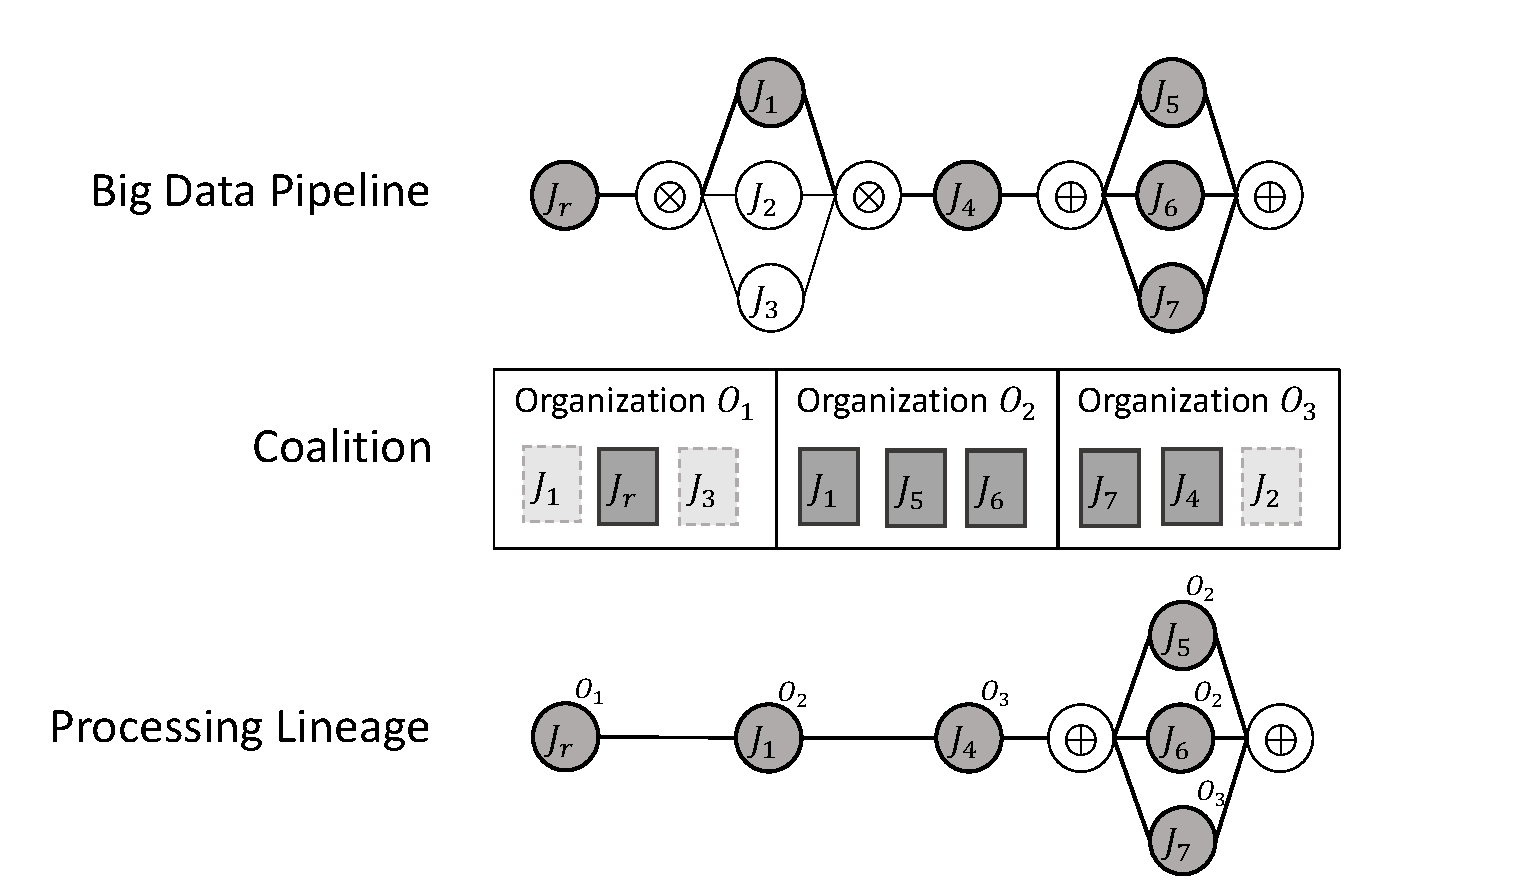
\includegraphics[width=0.98\columnwidth]{generaleFig1.pdf}
        \caption{Big Data Analytics pipeline graphs with a coalition of organization for a given processing lineage.}\label{fig:BDpipeline}
    \end{figure}
    
Figure~\ref{fig:BDpipeline} shows an overview of our system model.
In our model, organizations form coalitions, that is, collaborative networks of autonomous domains implementing a processing lineage of a given a Big Data analytics pipeline where resource sharing is achieved by the distribution of access permissions to coalition members based on negotiated resource-sharing agreements. A big Data pipeline can be constitute of a set of linear independent path (processing lineage) each of them implemented by coalition. In most cases, these coalitions are dynamic in nature, as changing conditions and trust relationships result in new missions and modifications to coalition membership. This scenario introduces a clear IT governance conflict: data should be compartmentalized to ensure strong protection, on one side, and shared to enable advanced analytics and key inter-organizational business processes, on the other side. This results in a set of strict requirements on existing access control systems that are discussed in the following section.

%Solid arrows present the typical batch or analytics model generation flows. Dashed arrows present typical streaming or prediction flows. \CH{togliere dalla figura la linea che separa le due procedure e le scritte ingestion procedure e analytics procedure?}
%The coalition creation is driven by missions including emergency and disaster management, humanitarian operations, or simply interdependent organizations.
%\CH{Qui ho introdotto solo il termine coalition, va spiegato anche il termine federation?}

\subsection{Requirements}\label{sec:accesscontrol_req}
%Rivisitazione dei requisiti di MEDES in ottica pipeline, coalizione etc.
The emerging need of balancing need to know/share and need to protect data in a coalition requires to rethink existing access control systems at the core of big data governance solutions. These solutions must consider the technical peculiarities of big data systems \cite{al2018exploring,aissa2020decide}, which point to scenarios where huge amount of data are diverse, come at high rates and must be proven to be trustworthy, as clarified by the 5V storyline \cite{5v}. In addition, they must take into account the increased governance complexity introduced by the collaborative environment. New  requirements then emerge as follows.
  
\noindent \textbf{[R1]}: Authorization should be the primary focus. Authentication is assumed to be managed by a separate and integrated module to guarantee federations within big data ecosystem. 
 
\noindent \textbf{[R2]}: Access control enforcement must protect data during their entire life cycle, along all processing phases, from ingestion to visualization, guaranteeing that data are properly protected and shared only to authorized users/organizations and for authorized operations. 

\noindent  \textbf{[R3]}: Along a big data pipeline, access to data must be evaluated before any operation on data takes place (guaranteeing a sort of \emph{least privilege} at each processing step).

\noindent \textbf{[R4]}: Access control enforcement should support fine-grained access control, dealing with both structured and unstructured data. When structured data are considered, policies should refer to a (set of) single cell, a column, a tuple or an entire table of structured data. When unstructured data are considered, policies should specify the portion of the unstructured file whose access need to be regulated. 

\noindent  \textbf{[R5]}: Access control policies must support the specification of dynamic context-based access conditions, that is, access rights might depend on the run-time characteristics of the big data system.

\noindent  \textbf{[R6]}: Access control policies must support the specification of dynamic access conditions based on the actual coalitions among organizations and their sharing agreement on both data and services.

\noindent  \textbf{[R7]}: Dealing with a collaborative environment, access control enforcement should not use data ownership as the only attribute to define access rights, but rather consider the evolving state of resources and processing services within a specific big data context. \CH{Qui volevo esprimere il fatto che i servizi eseguiti lungo la pipe possono appartenere a domini/organizzazioni diverse, che possono anche non essere i proprietari della risorsa, ma non ci sono riuscita}

\noindent  \textbf{[R8]}: In collaborative big data scenarios, where data are shared among large coalitions of different organizations, sensitive data should be exposed only to the level required for specific business needs, and according to coalition's sharing agreement and coalition's member privileges.

\noindent  \textbf{[R9]}: Access control should protect the privacy of sensitive data.

\noindent  \textbf{[R10]}: In collaborative big data scenarios, traditional accept-deny enforcement is not always possible/wanted especially in latency-sensitive scenarios. Deny access to data should be modeled as a data preparation job, transforming data according to privileges modeled in access control policies. %\CH{Aggiungere che nel contesto privacy basta trasformarla?}

\noindent \textbf{[R11]}: Access control enforcement should be highly efficient and scalable to accomplish the increasing cardinality of data and rate of requests.

\noindent \textbf{[R12]}: Access control enforcement should guarantee a proper balance between data share and data protection.

\section{Reference Scenario}\label{sec:reference}
TBW
\section{A Solution for Access Control in Big Data Scenarios}\label{sec:access}

Our methodology is based on two key pillars: on one side, we define an \textit{attribute-based access control model} that offers flexible fine grained authorization capabilities and exploits XACML notion of obligation to introduce preemptive data transformations that in a collaborative big data scenario are more suitable that denying data access.  On the other side,  differently from our previous work \cite{medes2021} where access control was done only at ingestion time, we monitor every data processing operation along the whole pipeline (see requirement {\bf R3}).

\subsection{Access Control Policy Model}\label{sec:ACmodel}

Recently, attribute-based access control has gained a lot of attention thanks to its highly customized ability to express dynamic and fine grained rules. Instead of assigning capabilities (i.e., action/object pairs) directly to a subject or to its role, policies rules specify under which conditions access is granted or denied. Rules are specified in terms of attributes of the subject, attributes of the object and environment conditions, with the advantage of allowing policies to be created and managed without direct reference to potentially numerous subjects and objects, and subject and objects to be provisioned without reference to a policy (requirement {\bf R6}). This approach also minimizes the number of policy rules needed (requirement {\bf R11}). Finally, by playing with attributes and environment conditions, we are able to express policies satisfying the requirements listed in Section \ref{sec:accesscontrol_req} and the peculiarities of big data scenarios. 

Our access control model then extends the policy structure of traditional attributed-based access control systems with two features:
\begin{itemize}
\item XACML optional obligations \cite{XACML3.0} specifying actions that must be performed before the policy is enforced and not directly associated with the controlled data become mandatory and are used to express data transformations that sanitize data resources to guarantee a minimum level of access to data. 
\item the evaluation of a policy rule always ends with an allow answer. Indeed, data protection is guaranteed by means of data transformations. 
\end{itemize}

As in any attribute-based access control model, the key elements of our model are defined as follows:
\begin{itemize}
\item XACML optional obligations \cite{XACML3.0} specifying actions that must be performed before the policy is enforced and not directly associated with the controlled data become mandatory and are used to express data transformations that sanitize data resources to guarantee a minimum level of access to data (requirement {\bf R8}). 
\item the evaluation of a policy rule always ends with an allow answer. Indeed, data protection is guaranteed by means of data transformations (requirement {\bf R10}). Obviously, deny access to data can happen in extreme cases when data transformations delete all data resources\footnote{In case of a data transformation function returning an empty dataset, the pipeline is not broken.}. 
\end{itemize}

As in any attribute-based access control model, the key elements of our model are defined as follows:
\begin{itemize}
\item A {\it subject} is a user or the service provider of a job that issues access requests to perform operations on objects. Subjects may have one or more attributes of the form (\textit{aname}, \textit{avalue}) pair, with \textit{aname} the name of the attribute and \textit{avalue} its value. In our case, there is always at least one attribute, specifying the organisation the subject belongs to. We use the notation \textit{u.aname} to refer to the value of attribute named \textit{aname}. For short, we use the notation $u@X$ to specify user $u$ belonging to organization $X$, i.e., to express the value of  \textit{u.organization}. 
\CH{credo abbia senso specificare dei subject predefiniti tipo any, none e admin, anche dei service provider predefiniti come kafka, hbase, hive. Lo faccio qui o nell'esempio?}

\item An {\it object} is any data whose access is governed by the policy (requirement {\bf R4}). It can be a file (e.g., a video, text file, image, etc.), a database, a table, a column, a raw, or a cell of a table. Like subjects, objects are assigned one or more attributes and have at least one, specifying the organization the object belongs to, expressed with the same notation $o@X$ for object $o$ belonging to organization $X$.

\item An {\it action} is any job that can be performed within a big data framework, ranging from classical atomic operations on a database (e.g, CRUD operations varying depending on the data model) to coarser operations such as an Apache Spark DAG, an Hadoop MapReduce, an analytics function call, or a pipe offered by a different service provider. 

\item The {\it environment} is defined by a set of dynamic attributes related to the specific context, such as time of the day, location, ip address, risk level, etc. \CH{mettere degli attributi piu' sensati, come normal e critical situation}. 

\end{itemize}

The access control policy is then defined as a set of policy rules expressing access conditions based on the key elements and their attributes. As mentioned earlier, the novelty of our model is in the exploitation of suitable data transformation functions that are applied to the target resource in order to sanitize it before access is given (requirement {\bf R8}).
As a consequence, when a subject makes an access request to a resource (i.e., an object), the policy rule matching the access request is evaluated, and the access is given after one or more data transformations are performed (requirement {\bf R10}). Obviously, deny access to data can happen in extreme cases when data transformations delete all data resources\footnote{In case of a data transformation function returning an empty dataset, the pipeline is not broken.}. 



\begin{definition}[Policy Rule]
A {\it policy rule} is a predicate {\it policy\_rule$_{obj}$(subj, action, env, datatrans)} defined as:
\begin{verbatim}
if (cond_expr == true)
then datatrans
\end{verbatim}
where {\tt cond\_expr} is a propositional boolean expression built on composition of mathematical operators ($>,<, =, +, -, *, /$), logical operators ($\land,\lor,\neg$), set operators ($\in,\subset,\subseteq,\supset, \supseteq \cup,\cap$) and logical quantifiers ($\forall, \exists$) on the resource \textit{obj} and on arguments \textit{subj}, \textit{action} and \textit{env} and their attributes. \texttt{datatrans} are functions transforming da\-ta resources in different ways, mainly to protect against information leakage. \CH{da sistemare rendendo piu' leggibile, da decidere se va bene che i permessi siano dati come ACL}
\end{definition}

Transformation functions range from pruning and reshaping to encrypting/decrypting or anonymizing the full resource or part of it. Thus, data protection is obtained by removing or obfuscating sensitive attributes rather than denying access to full data. In section \ref{sec:dataTransformations}, we define a taxonomy of data transformations based on the security property that has to be guaranteed.
The transformation function can be applied to the full resource or to part of it, either a single attribute or a set of attributes. For example, in case of structured data it can be applied to a single cell, to (one or more) rows or columns, either to the entire table. The target of the transformation function is given as parameter to the function.

In attribute-based access control model, policies are limited only by the computational language and the richness of the available attributes. In our case, we exploit the {\it environment} field of our model to contain the dynamic information on actual coalitions to express coalitions.

\begin{definition}[Coalition]
A coalition $C$ is a set of organizations $o\in O$, with $O$ the set of the organizations associated to the specific scenario.
\end{definition}
The {\it environment} field of our model then contains both $O$ and the actual coalitions. Given an organization $o$ o, function $\textit{Coalition}(O)$ returns the set of coalitions an organization $o\in O$ is part of, i.e, $\textit{Coalition}(o)=\{ C | o \in C\}$. In a coalition resource sharing is achieved by the distribution of access permissions to coalition members. In order to simplify and speed up policy writing, it is common to define a default set of permissions rules to be applied to all coalition members. This set of rules are part of a coalition agreement.

\begin{definition}[Coalition Agreement]
A \textit{coalition a\-greement} $\textit{CA}_C$ is a set of policy rules associated to a coalition $C$ that are added to the security policy of each organization.
\end{definition}
Obviously, the rules of a coalition agreement depend on the specific nature of a coalition. For example, given a coalition $C$ between organisations that do not handle sensitive data, a default rule in the coalition agreement could be:
\vspace{0.3cm}

\noindent $\textit{policy\_rule}_{obj}(\textit{subj},\texttt{any},\textit{env},\texttt{-}) \equiv \textit{obj.organization} \in C  
 \land \textit{subj.organization} \in C 
$
\vspace{0.3cm}

\noindent expressing the fact that subjects belonging to the same coalition can have access to all data (\texttt{-} means that no transformation functions are performed before access is given).
\hl{L'esempio sotto dovrebbe parare di coalizione e coalition agreement no?}
\begin{example}
Let us consider an healthcare scenario, with an hospital $A$ storing patients' information such as patient personal information (e.g., social security number, home address, healthcare insurance, etc.), medical journals and medication records. We suppose there are three different roles among the hospital staff: doctor, nurse and administrative staff. 
They all need to access patient's data in their daily activities, but it would make sense to have specific access rules based on the role, such as:
\begin{itemize}
\item a doctor can have access only to medical journals and medication records;
\item a nurse should only have read access on medication records;
\item an administrative must have access only to patient's personal information.
\end{itemize}
In our model, we can specify the three roles as subject's attribute \textit{role}
which can have only one of three values \texttt{doctor}, \texttt{nurse}, and \texttt{admin}. Then, we can express the three policy rules as:

\vspace{0.3cm}

\noindent $\textit{policy\_rule}_{PatientData}(\textit{s},\texttt{any},\textit{env},\texttt{-}) \equiv \textit{s.role} = \texttt{doctor}
$
\vspace{0.3cm}

\noindent $\textit{policy\_rule}_{PatientData}(\textit{s},\texttt{READ},\textit{env},\texttt{medication only}) \equiv \textit{s.role} = \texttt{nurse}
$
\end{example}

\subsection{Data Annotation}

In cloud scenarios, it is common to apply metadata tags to resources to perform more sophisticated filtering or reporting on resources. A tag is a label consisting of a key and an optional value that is assigned to a resource. In our case, we exploit tagging to specify attributes of subjects, resources or contextual information. Using data annotation to enforce data protection policies has three major advantages: \begin{enumerate}
\item Metadata tagging permits to extract value also out of possibly unstructured ingested raw data. For example, it is possible to capture document semantics through tags. Thus, tagging helps in defining policies at different levels of granularity, also in case of unstructured data.
\item Tagging enables to categorize resources in different ways (e.g, by purpose, owner, environment, or other criteria), encompassing conventional database schema information. Even relationships between attributes of different data sets can be indicated as tags, without the need of, computationally expensive, data normalization. 
\item Tags can also be used to express access control related attributes, such as data sensitivity or multi-level security policies by means of owner-defined security levels, or role-based policies. 
\end{enumerate}

When using tagging for access control in a distributed scenario, it is important to devise a consistent set of tag keys, that is, a common vocabulary. However, which tags to apply to which resources differs depending on the specific use case, working environment, or context.  Table~\ref{tab:tags} provides an example of a common vocabulary at the basis of tag-based access control policies. For instance, use case {\em privacy classification} should be used every time data privacy must be protected, that is, every time personal data are involved. Data privacy generally refers to the ability of a person to determine when, how, and to what extent her personal information can be shared with or communicated to others. According to the General Data Protection Regulation (GDPR) \cite{EUdataregulations2018}, personal data are any information relating to an identified or identifiable natural person (called data subject). Based on this definition and on the technological advances that have improved data collection and analytics, personal data (Personally Identifiable Information - PII) fall into three categories: {\em i)} explicit identifiers, any information that directly identifies individuals with certainty, such as national ID, assurance number, phone number, passport number; {\em ii)} quasi identifiers, a set of data attributes that could jointly or uniquely identify a subject when combined with publicly available data, such as ZIP code, date of birth, and address; {\em iii)} sensitive information, data related to a person without directly identifying her but that, if linked to an individual, reveals sensitive aspects of her private life (e.g., religion belief, health information, legal issues).







\subsection{Data Transformation}\label{sec:dataTransformations}




\subsection{Access Control Enforcement}
Figure~\ref{fig:smet} shows how the access control model presented in section \ref{sec:ACmodel} is integrated in the big data processing system of Figure~\ref{fig:BDpipeline}. 

\begin{figure}[!t]
	\centering
	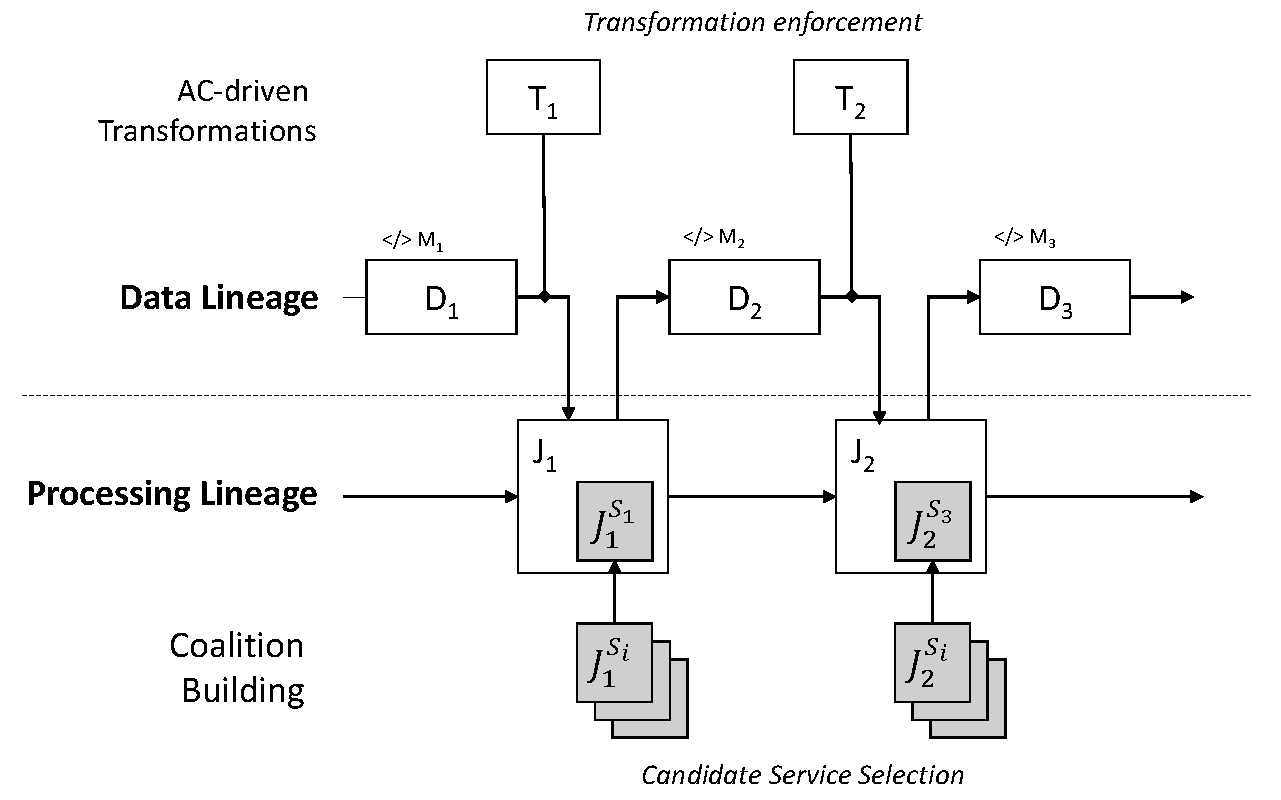
\includegraphics[width=0.48\textwidth]{meth.pdf}
\caption{Access Control Enforcement process.}
	\label{fig:smet}
\end{figure} 


Data lineage is a set of complex relationships between datasets $D_i$ and jobs $J_i$ in a pipeline.  The picture shows how policy enforcement works along the data lineage obtaining data protection by means of AC and transformations prior to feed data to a processing job.
Along the pipeline, with data flowing from data sources to computation, access control enforcement works as follows:
\begin{enumerate}
\item When $D_i$ has to be processed by job $J_i$ provided by a service provider $S_j$, an access decision has to be taken.
\item A matching rule $\textit{policy\_rule}_{D_i}(S_j,J_i,\textit{env})$ is searched in the policy, considering all the actual values of the attributes of both subjects and objects. If the rule is found, the corresponding data transformation $T_1$ is performed.
\item Job $J_i$ is executed on $D_i$ after the transformation, generating $D_{i+1}$ that go through the same process before being fed to job $J_{i+1}$.
\end{enumerate}


%Il dato arriva gia' annotato e i job eventualmente sono in grado di modificare l'annotazione
\section{Architectural Deployment}\label{sec:architecture}
We present the architectural deployment of our access control system discussing two possible approaches: \emph{i)} centralized deployment; \emph{ii)} decentralized deployment. The choice of the specific deployment has an impact on the way in which the coalition \coalition{} of organizations \org{i} is formed as discussed in the following of this section.

\begin{figure*}[!t]
    \begin{tabular}{cc}
        \parbox[]{10cm}{~\\~\\~\\~\\~\\~\\~\\~\\~\\~\\}&\parbox[]{10cm}{~\\~\\~\\~\\~\\~\\~\\~\\~\\~\\}\\
        (a)&(b)\\
    \end{tabular}
    \caption{Centralized (a) and decentralized (b) deployment}
\end{figure*}

\subsection{Centralized Deployment}\label{sec:centralized}
A centralized deployment implements a service orchestration, where an orchestrator \orc\ provides access control functionalities and mediates access from organization \org{i} in \coalition{} to a given dataset \dataset{}. A service orchestration can be formally defined as follows.

\begin{definition}\label{def:orchestration}
    Given a big data analytics pipeline \G(\V,\E) in Definition \ref{def:pipeline}, a coalition \coalition{} of organizations \org{i}$\in$\Org{} each implementing a job \job{i}, a dataset \dataset{}, and an orchestrator \orc{}, a service orchestration is a direct acyclic graph \G$^c$(\V$^c$,\E$^c$), where \V$^c$=\V$_I$$\cup$\orc{} and \E$^c$=\{\vi{i},\orc{}\}$\cup$\{\orc{},\vi{i}\}, with \vi{i}$\in$\V$^c$ modeling a job \job{i}. 
\end{definition}

We note that each communication between two subsequent jobs \job{i-1} and \job{i} in \coalition{} is mediated by the orchestrator, which enforces all applicable policies. We also note that vertices \vi{c} and \vi{m} of an alternative structure, as well as \vi{f} and \vi{j} of a parallel structure, are included in the orchestrator \orc{}. Two enforcement processes are implemented in the centralized deployment as follows.
\begin{enumerate}
    \item \textbf{Incoming enforcement.} Policy enforcement is done by the orchestrator before dataset \dataset{} is released to a specific (set of) job \job{i}. It is then executed for each edge \{\orc{},\job{i}\} and decrease or maintain the utility of the dataset (i.e., the enforcement has no impact on the dataset or remove some information).
    \item \textbf{Outgoing enforcement.} Policy enforcement is done by the orchestrator after a resulting dataset \dataset{} is returned by a specific (set of) job \job{i}. It is then executed for each edge \{\job{i},\orc{}\} and aims to restore those data that were manipulated before access by \job{i-1}. In other words, once the resulting dataset is returned by \job{i-1}, orchestrator \orc{} restore those data that were not accessible by \job{i-1} (e.g., by deanonymizing it).
\end{enumerate}

We note that centralized deployment maximizes the utility of the dataset providing each job with the largest amount of data possible, meaning that data transformation assumes a non-monotonic behavior. It is a single point of failure and assumes all jobs to coexist in a single environment. Generalization to multiple environments is possible but outside the scope of this paper.

\subsection{Decentralized Deployment}\label{sec:decentralized}
A decentralized deployment implements a service choreography, where organization \org{i} in \coalition{} are directly connected and exchange data. A service choreography can be formally defined as follows.

\begin{definition}\label{def:choreography}
    Given a big data analytics pipeline \G(\V,\E) in Definition \ref{def:pipeline}, a coalition \coalition{} of organizations \org{i}$\in$\Org{} each implementing a job \job{i}, and a dataset \dataset{}, a service choreography is a direct acyclic graph \G$^d$(\V$^d$,\E$^d$), where \V$^d$=\V\ and \E$^d$=\{\vi{i},\vi{j}\} with \vi{i}$\in$\V$^d$ modeling a job \job{i}. 
\end{definition}

We note that each communication between two subsequent jobs \job{i-1} and \job{i} in \coalition{} is direct with no mediation. Each job is complemented with an external plugin enforcing all applicable policies. Policy enforcement is done by the plugin of \job{i-1} before dataset \dataset{} is released to job \job{i}. It is then executed for each edge \{\job{i-1},\job{i}\}, enforcing all applicable policies and decrease or maintain the utility of the dataset (i.e., the enforcement has no impact on the dataset or remove some information). We note that decentralized deployment provides a data transformation assuming a not-increasing monotonic behavior. Communications are distributed among different job platforms requiring data transfer during analytics. This choice could decrease performance when huge datasets must be distributed. 

\section{Coalition Building}\label{sec:coalition}
Coalition building is a crucial process having direct impact on the quality of the analytics results. Figure~\ref{fig:smet} shows how data lineage is impacted by the processing lineage and in particular by i) the \textit{coalition a\-greement} $\textit{CA}_C$ (i.e., the CA-driven transformations adopted for a give coalition) and by ii) the transformation produced by the different jobs (job-specific transformation) part of a given coalition \coalition{}.
Let us consider job $\job{1}^{\org{1}}$ of Figure~\ref{fig:smet} it receives as input the data \trans{1}(\dataset{1}) based on the dataset obtained by \dataset{1} after the transformation  \trans{1} which is associated to the data lineage by our AC model. It then produce a data that is the job-specific transformation on the input data (i.e., \trans{1}(\dataset{1})) generating \dataset{2}.
We note that our Big Data Analytics pipeline models includes alternatives allowing different processing lineage (linear independent path in the Big data graph G) doing the same analytics but using different jobs (e.g., a lineage including k-means or a lineage using c-means). This will lead to different job-specific transformation on the data for the same Big Data pipeline.
In this paper, for the sake of simplicity we i) consider different coalitions for each processing lineage, ii) coalitions made of trustworthy organizations \org{i} providing candidate services for each job and iii) job-specific transformation not influenced by the organizations' behavior.
In this scenario, since any coalition of a given processing lineage will produce the same job-specific data transformation, the analytics pipeline quality is impacted only by the \textit{coalition agreement} $\textit{CA}_C$ or rather by the transformations \trans{i} imposed by the given coalition \coalition{} on the data lineage.
In the following we first present metrics to evaluate data quality across the data lineage, and then a set of solutions to build coalitions for  given Big Data pipeline ensuring a given data quality.

%\begin{example}\label{ex:p1j}
%The choice of the specific deployment has an impact on the way in which the coalition \coalition{} of organizations \org{i} is formed as discussed in the following of this section.
%Let us consider the following example where we have a pipeline made of just one ingestion job that can be offered by service provider $s_1$ or by the service provider $s_2\] In case the $s_1$ is selected the transformation $T_1$ is triggered according to the authorization $s_1$ has on the data, in this example $s_1$ has full control meaning that transformation $t_1$ is empty. In case the $s_2$ is selected the transformation $T_2$ is triggered according to the authorization $s_2$ has on the data and in this example data labelled as PII are removed.
%\end{example}
%Considering the two data lineage generated by the two different coalition in Example\ref{ex:p1j} the one involving $s_2$ produce a significant changes to data compared to the other one. This data changes can have direct impact on the quality of the analytics outcomes, therefore our goal is to build coalitions ensuring specific data quality. This coalition building problem can be assimilated to xxx showing an exponential complexity ...
%In the following we fist introduce our data quality metrics and then our euristics to solve the problem of coalition building

%\subsection{Data Quality metrics}
%\subsection{Coalition Heuristics}
\subsection{Metrics}

Data quality is a largely studied topic for the database management research communities,
and is in general focused on the quality of the data source rather then on the quality of the data outcomes or of the data while used in the processing pipeline.
In \cite{BigDataQaulitySurvey} a survey on big data quality is proposed mentioning the well known categories of big data quality grouped by intrinsic,
contextual representational and accessibility categories.

It also presents an holistic quality management model where the importance of data quality during processing is just mentioned in terms of requirements for the pre-processing job (e.g., data enhancement due to cleaning jobs).
In this paper we depart from this idea on data quality at pre processing time only measuring it at each step of the big data pipeline.
%data quality are divided into four categories: intrinsic, contextual representational and accessibility that covers almost all the aspects of data at ingestion time


In the following we present a set of metrics to evaluate the quality of the data at each step of the big data pipeline.
We

The proposed metrics can be classified into two categories, namely quantitative and statistical.
Initially, these metrics are applied to the original dataset (X) without any transformations, and subsequently, they are applied to the transformed dataset (Y).
The quantitative approach facilitates the calculation of the amount of data that has been lost during the transformation by enumerating the differences between X and Y.
On the other hand, the statistical approach takes into consideration the changes in certain statistical properties before and after the transformation.
These metrics can be applied either to the entire dataset or specific features.
The features can be assigned either equal or varying weights, which enables the prioritization of important features that were lost during the transformation.

% \item Metrica quantitativa
% \item Mean Squared Error (MSE). Let us considera two dataset X and Y of the same size. The MSE is defined as: $MSE(X,Y) = \frac{1}{n}\sum_{i=1}^{n}(x_i - y_i)^2\]
% \item Metrica quantitativa pesata
% \item Parametri statistici (deviazione standard, media, ecc)

\subsubsection{Jaqard coefficent}
Let us consider two dataset X and Y of the same size.
The Jaqard coefficent is defined as:\[J(X,Y) = \frac{|X \cap Y|}{|X \cup Y|}\]
The use of Jaccard coefficient has several advantages when applied to datasets.
Unlike other similarity measures, such as Euclidean distance, Jaccard coefficient is not affected by the magnitude of the values in the dataset.
This property makes it suitable for datasets with categorical variables or nominal data, where the values do not have a meaningful numerical interpretation.
The coefficient ranges from 0 to 1, where 0 indicates no similarity and 1 indicates complete similarity between the sets.
\subsubsection{Jaqard coefficent with weights} Let us consider two dataset X and Y of the same size. The Jaqard coefficent is defined as:\[J(X,Y) = \frac{\sum_{i=1}^{n}w_i(x_i \cap y_i)}{\sum_{i=1}^{n}w_i(x_i \cup y_i)}\]
Weighted Jaccard similarity is a variant of the Jaccard coefficient that incorporates weights to the elements in the sets being compared.
It allows for the prioritization of certain features or elements in the datasets.
This approach can be particularly useful when some elements in the dataset have more importance or relevance than others.
By assigning weights to the elements, the weighted Jaccard similarity can account for this importance and provide a more accurate measure of similarity.
\subsubsection{Kullback-Leibler divergence} Let us consider two dataset X and Y of the same size. The KL divergence is defined as:\[KL(X,Y) = \sum_{i=1}^{n}x_i \log \frac{x_i}{y_i}\]
The KL divergence is a measure of the difference between two probability distributions and is useful for comparing the dissimilarity of two datasets.


\subsubsection{Kullback-Leibler divergence with weights} Let us consider two dataset X and Y of the same size. The weighted KL divergence is defined as:

\[KL(X,Y) = \sum_{i=1}^{n}w_i(x_i \log \frac{x_i}{y_i})\]

The weighted KL divergence is a variant of the KL divergence that incorporates weights to the elements in the datasets being compared.
It allows for the prioritization of certain features or elements in the datasets.
This approach can be particularly useful when some elements in the dataset have more importance or relevance than others.
By assigning weights to the elements, the weighted KL divergence can account for this importance and provide a more accurate measure of dissimilarity.

\subsection{Euristics}
The metrics established will enable the quantification of data loss pre- and post-transformations.
In the event of multiple service interactions, each with its respective transformation, efforts will be made to minimize the loss of information while upholding privacy and security standards.
Due to the exponential increase in complexity as the number of services and transformations grow, identifying the optimal path is inherently an NP-hard problem.
As such, we propose some heuristics to approximate the optimal path as closely as possible. To evaluate their efficacy, the heuristically generated paths will be compared against the optimal solution.
\begin{description}
    \item[Greedy] The greedy algorithm is a heuristic that can be used to minimize the quantity of information lost by making locally optimal choices at each step in the hope of achieving a globally optimal solution.
        For instance, in our service selection problem, the greedy algorithm can be used to select services in order of their information loss, starting with the service with the lowest information loss.
        This strategy ensures that services with lower information loss are selected first, minimizing the overall quantity of information lost.
    \item[Sliding Window] The sliding window algorithm is a heuristic that can be used to minimize the quantity of information lost by considering a subset of the available services defined by a fixed or moving window.
        For example, in our service selection problem where the quantity of information lost needs to be minimized, the sliding window algorithm can be used to select services composition that have the lowest information loss within a fixed-size window.
        This strategy ensures that only services with low information loss are selected, minimizing the overall quantity of information lost.
\end{description}
The utilization of heuristics in service selection can be enhanced through the incorporation of techniques derived from other algorithms, such as Ant Colony Optimization or Tabu Search.
By integrating these approaches, it becomes feasible to achieve a more effective and efficient selection of services, with a specific focus on eliminating paths that have previously been deemed unfavorable.
\subsubsection{pensieri di Ernesto}
\begin{itemize}
    \item In sede di ingestion, la valutazione sull'impatto dell'analitica la posso fare. Se privacy e valori numerici si può compiare epsilon e delta di differential privacy (noise addition o allargare la distribuzione di rumore sulla base del budget di privacy).
    \item Metriche quantitative, come ricercar potrebbe essere interessante schema di budget di privacy per l'offuscamento di dati non numerici Quante volte il dato viene trasformato
    \item Analitiche di statistica descrittiva per il 3sigma -> piattaforma di puliafito (Catania)
    \item Anomaly detection con deviazione standard
    \item Data sanitizzato fa il merge di due barre dell' istogramma è un' autoencoding, come cambia la deviazione standard
\end{itemize}

\section{Experiments}\label{sec:experiment}
We experimentally evaluated the performance and quality of our methodology (heuristic algorithm in \cref{subsec:heuristics}), and compared it against the exhaustive approach in~\cref{sec:nphard} {\color{OurColor}and our baseline modeling solutions in the state of the art in~\cref{subsec:experiments_infrastructure}.} In the following,
\cref{subsec:experiments_infrastructure} presents the simulator and experimental settings used in our experiments;
\cref{subsec:experiments_performance} analyses the performance of our solution in terms of execution time; \cref{subsec:experiments_quality} discusses the quality of the best pipeline instance generated by our solution according to the metrics $M_J$ and $M_{JSD}$ in \cref{subsec:metrics}.

\subsection{Testing Infrastructure and Experimental Settings}\label{subsec:experiments_infrastructure}
Our testing infrastructure is a Swift-based simulator of a service-based ecosystem, including service execution, selection, and composition.
The simulator first defines the pipeline template as a sequence of $l$ vertices, with $l$ the length of the pipeline template, and defines the size \windowsize\ of the sliding window, such that \windowsize$\leq$$l$. We recall that alternative vertices are modeled in different pipeline templates, while parallel vertices are not considered in our experiments since they only add a fixed execution time that is negligible and does not affect the performance and quality of our solution. Each vertex is associated with a (set of) policy that applies a filtering transformation that removes a given percentage of data.


      The simulator then starts the instantiation process. At each step $i$, it selects the subset \{\vi{i},$\ldots$,$v_{\windowsize+i-1}$\} of vertices with their corresponding candidate services, and generates all possible service combinations. The simulator calculates quality $Q$ for all combinations and instantiates \vi{i} with service \sii{i} from the optimal combination with maximum $Q$. The window is shifted by 1 (i.e., $i$=$i$+1), and the instantiation process restarts. When the sliding window reaches the end of the pipeline template, that is, $v_{\windowsize+i-1}$$=$$\vi{l}$, the simulator computes the optimal service combination and instantiates the remaining vertices with the corresponding services. \cref{fig:execution_example} shows an example of a simulator execution with $i$$=$2 and \windowsize$=$3. Subset \{\vi{2},\vi{3},\vi{4}\} is selected, all combinations generated, and corresponding quality $Q$ calculated. Optimal service combination \{\sii{11},\sii{22},\sii{31}\} is retrieved and \vii{2} in the pipeline instance instantiated with \sii{11}.

    \begin{figure}[!t]
      \centering
      \resizebox{0.7\columnwidth}{!}{%
        \begin{tikzpicture}[framed]

          \node[draw, circle, fill=gray!40,minimum width=0.7cm] (v1) at (1,5.2) {$\vi{1}$};
          \node[draw, circle, fill=gray!40,minimum width=0.7cm] (v2) at (3,5.2) {$\vi{2}$};
          \node[draw, circle, fill=gray!40,minimum width=0.7cm] (v3) at (5,5.2) {$\vi{3}$};
          \node[draw, circle, fill=gray!40,minimum width=0.7cm] (v4) at (7,5.2) {$\vi{4}$};
          \node[draw, circle, fill=gray!40,minimum width=0.7cm] (v5) at (9,5.2) {$\vi{5}$};
          \node[above, shift=({0,0.5}),  ] at (v3.north)  {Sliding Window};

          \node[draw, rectangle,fill=red!20] (s1) at (1,3.4) {$\sii{1}$};
          \node[draw, rectangle, fill=green!20] (s2) at (1,1.7) {$\sii{2}$};
          \node[draw, rectangle, fill=red!20] (s3) at (1,0) {$\sii{3}$};

          \node[draw, rectangle,thick] (s11) at (3,3.4) {$\sii{11}$};
          \node[draw, rectangle,opacity=.6] (s12) at (3,1.7) {$\sii{12}$};
          \node[draw, rectangle,opacity=.6] (s13) at (3,0) {$\sii{13}$};

          \node[draw, rectangle,opacity=.6] (s21) at (5,3.4) {$\sii{21}$};
          \node[draw, rectangle,thick] (s22) at (5,1.7) {$\sii{22}$};
          \node[draw, rectangle,opacity=.6] (s23) at (5,0) {$\sii{23}$};

          \node[draw, rectangle, thick] (s31) at (7,3.4) {$\sii{31}$};
          \node[draw, rectangle,opacity=.6] (s32) at (7,1.7) {$\sii{32}$};
          \node[draw, rectangle,opacity=.6] (s33) at (7,0) {$\sii{33}$};

          \node[draw, rectangle] (s41) at (9,3.4) {$\sii{41}$};
          \node[draw, rectangle] (s42) at (9,1.7) {$\sii{42}$};
          \node[draw, rectangle] (s43) at (9,0) {$\sii{43}$};

          \draw[->,line width= 1.2pt] (s2) -- (s11);
          \draw[->,dashdotted] (s2) -- (s12);
          \draw[->,dashdotted] (s2) -- (s13);

          \draw[->,line width= 1pt] (s11) -- (s22);

          \draw[->,dashdotted] (s11) -- (s21);
          \draw[->,dashdotted] (s11) -- (s23);

          \draw[->,dashdotted] (s12) -- (s21);
          \draw[->,dashdotted] (s12) -- (s22);
          \draw[->,dashdotted] (s12) -- (s23);

          \draw[->,dashdotted] (s13) -- (s21);
          \draw[->,dashdotted] (s13) -- (s22);
          \draw[->,dashdotted] (s13) -- (s23);

          \draw[->,dashdotted] (s21) -- (s31);
          \draw[->,dashdotted] (s21) -- (s32);
          \draw[->,dashdotted] (s21) -- (s33);

          \draw[->,line width=1pt] (s22) -- (s31);
          \draw[->,dashdotted] (s22) -- (s32);
          \draw[->,dashdotted] (s22) -- (s33);

          \draw[->,dashdotted] (s23) -- (s31);
          \draw[->,dashdotted] (s23) -- (s32);
          \draw[->,dashdotted] (s23) -- (s33);

          \draw[->] (v1) -- (v2);
          \draw[->] (v2) -- (v3);
          \draw[->] (v3) -- (v4);
          \draw[->] (v4) -- (v5);

          \begin{scope}[on background layer]
            \draw[thick, dashed, fill=red!10, opacity=0.5]
            ([shift={(-0.5,0.5)}]s11.north west) rectangle ([shift={(0.5,-0.5)}]s33.south east);

          \end{scope}
          \begin{scope}[on background layer]
            \draw[thick, dashed, fill=red!10, opacity=0.5]
            ([shift={(-0.5,0.5)}]v2.north west) rectangle ([shift={(0.5,-0.5)}]v4.south east);

          \end{scope}

        \end{tikzpicture}
      }
      \caption{Execution example of the sliding window heuristic using v=5, s=3, \windowsize=3 at i=1 step.}
      \label{fig:execution_example}
    \end{figure}

    The simulator defines dependencies between filtering transformations made by candidate services at consecutive vertices of the pipeline template.
    To this aim, it assigns a dependency rate to each service \si{i} modeling the amount of the filtering transformation done at \si{i} that overlaps the one at \si{i-1}.
    For example, let us consider the pairs of services (\si{11},\si{21}) and (\si{11},\si{22}) with the following configurations: \emph{i)} service \si{11} introduces a filtering transformation that removes the 20\% of the dataset, \emph{ii)} service \si{21} introduces a filtering transformation that removes 10\% of the dataset and has dependency rate equal to 1, meaning that the filtering transformation made by \si{21} completely overlaps the one made by \si{11}, \emph{iii)} service \si{22} introduces a filtering transformation that removes 5\% of the dataset and has dependency rate equal to 0.5, meaning that the filtering transformation made by \si{22} overlaps half of the one made by \si{11}. Jaccard Metric $M_{J_{21}}$$=$0.8 at service \si{21}; $M_{J_{22}}$$=$0.775 at \si{22}, showing how dependencies can affect the pipeline quality and, in turn, the instantiation process.


    Our simulator also supports the comparison of the performance and quality of our sliding-window heuristic with \emph{i)} a baseline modeling solutions in the state of the art and \emph{ii)} the exhaustive approach (i.e., the theoretical optimum). We modeled our baseline as a greedy approach that, for each node of the service pipeline, selects the best service that maximizes the data quality, while addressing data protection requirements in annotation $\myLambda$. The reason is that, to the best of our knowledge, existing (industry) solutions and standards do not support service-based data pipelines and are therefore unable to instantiate the service pipeline according to the pipeline structure and service dependencies. We therefore defined our baseline as the sliding window heuristic configured with window size $|$w$|$=1.
    We implemented the exhaustive approach calculating the theoretical optimum as the sliding window heuristic configured with window size $|$w$|$=$l$, to illustrate the potential efficiency of our heuristics within realistic computational limits.

    \begin{table}[!t]
      \caption{Experimental Parameters}
      \label{tab:parameters}
      \centering
      {\color{OurColor2}
        \begin{tabular}{l|l}
          \textbf{Parameter}                   & \textbf{Values}                               \\
          \hline
          Window Size \textbar{}w\textbar{}    & 1, 2, 3, 4, 5, 6, 7                           \\
          Pipeline Template Length $l$         & 3, 4, 5, 6, 7                                 \\
          Number of Candidate Services $|S^c|$ & 2, 3, 4, 5, 6, 7                              \\
          Filtering Configuration              & wide, average                                 \\
          Metric                               & quantitative ($M_J$), qualitative ($M_{JSD}$) \\
        \end{tabular}
      }
    \end{table}
    {\color{OurColor2}
    \cref{tab:parameters} outlines the parameters and corresponding values used in our experimental evaluation. Paremeter \emph{Window Size} (\textbar{}w\textbar{}), varying from 1 to 7, models different configurations of our heuristic. Parameter \emph{Pipeline Template Length $l$}, varying from 3 to 7, models the depth of the pipeline template as the number of vertices composed in a sequence. Parameter \emph{Number of Candidate Services $|S^c|$}, varying from 2 to 7, models the number of alternative services at each vertex of the pipeline template. Parameter \emph{Filtering Configuration} considers two representative filtering transformations: \textit{wide} removing a percentage of data in [0.2,1] and \textit{average} in [0.5,0.8]. Parameter \emph{Metric} considers two quality metrics: quantitative ($M_J$) and qualitative ($M_{JSD}$).}

    Our experiments have been run on a virtual machine equipped with an Intel(R) Xeon(R) CPU E5-2620 v4 @ 2.10GHz CPU and 32GB RAM. Each experiment was repeated 10 times and the results averaged to improve the reliability of findings.

    \begin{figure}[!ht]
      \centering
      \begin{subfigure}{0.45\textwidth}
        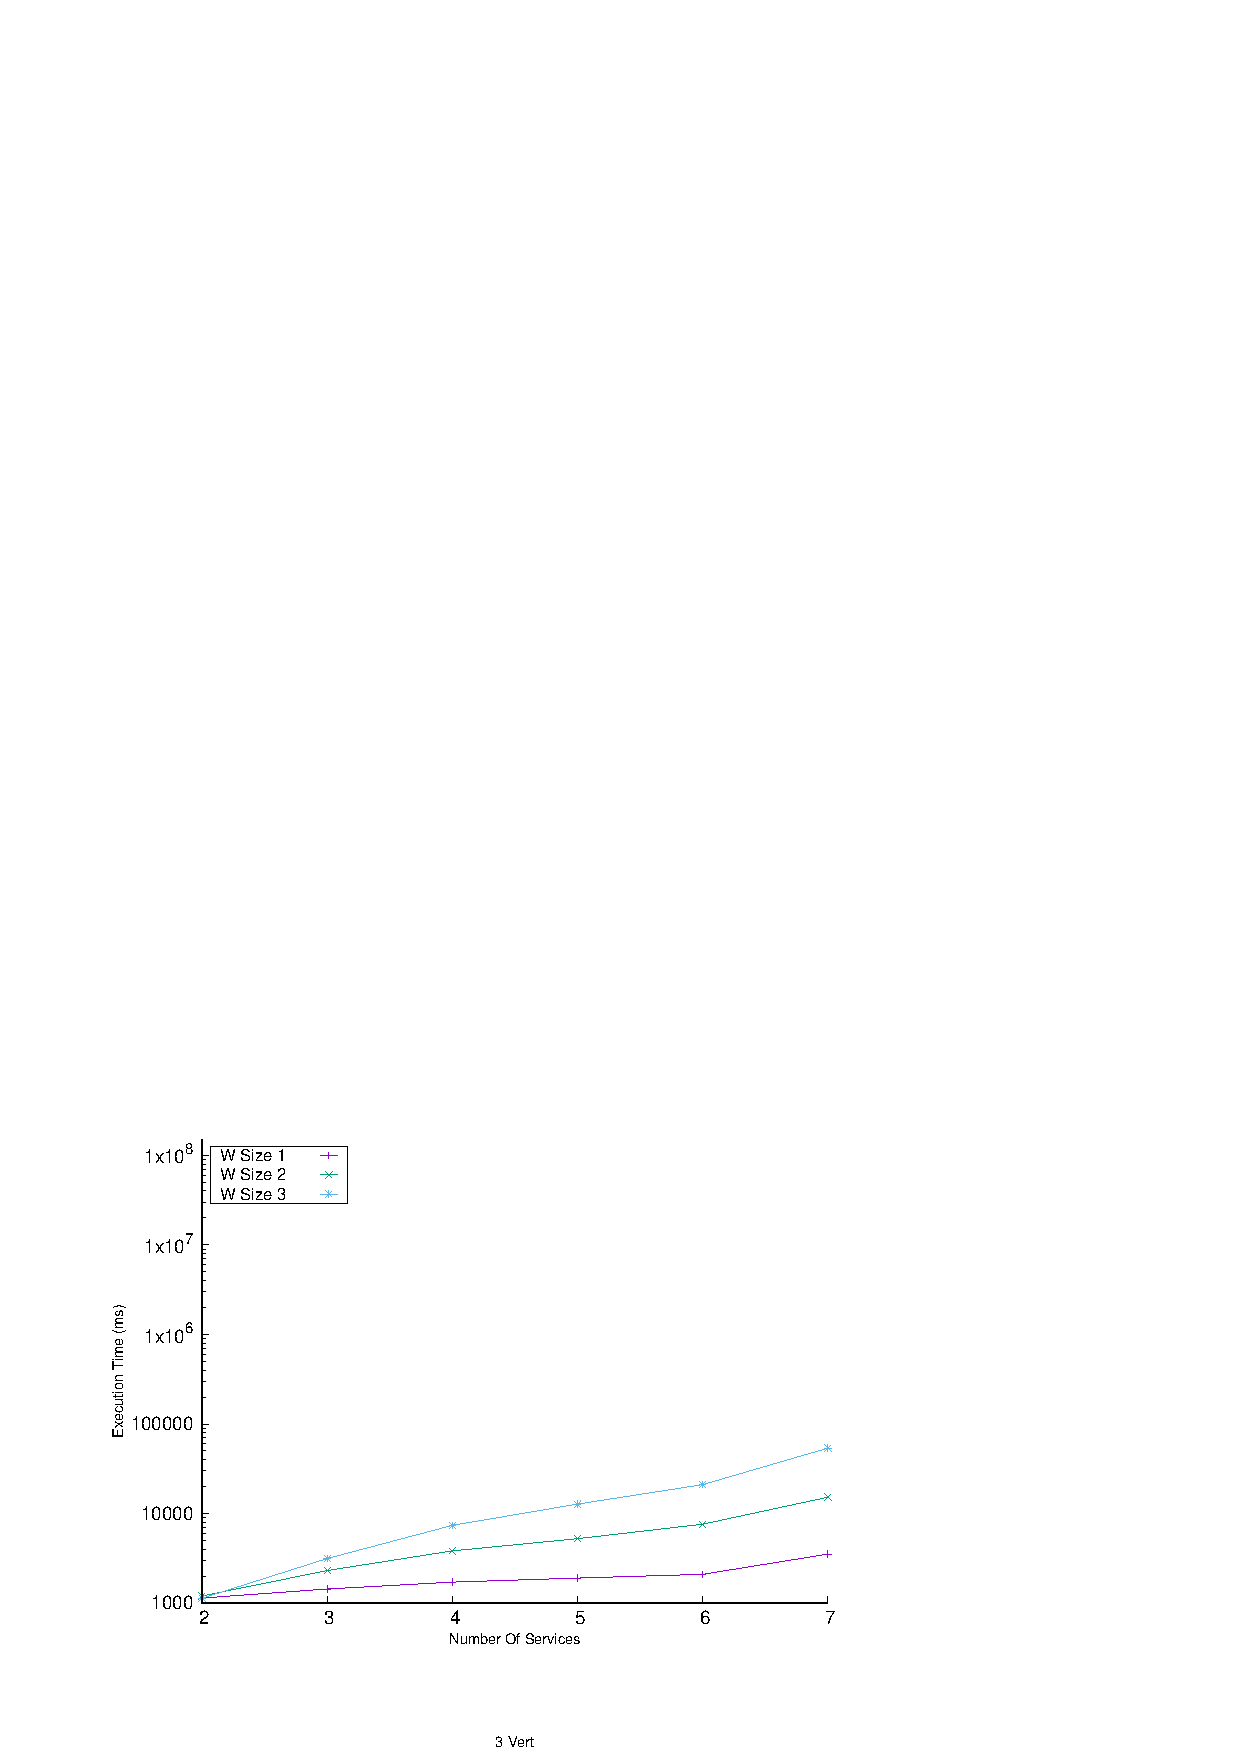
\includegraphics[width=\textwidth]{Images/graphs/window_time_performance_qualitative_n7_s7_50_80_n3}
        \caption{3 vertices}
        \label{fig:time_window_perce_wide_3n}
      \end{subfigure}
      \hfill
      \begin{subfigure}{0.45\textwidth}
        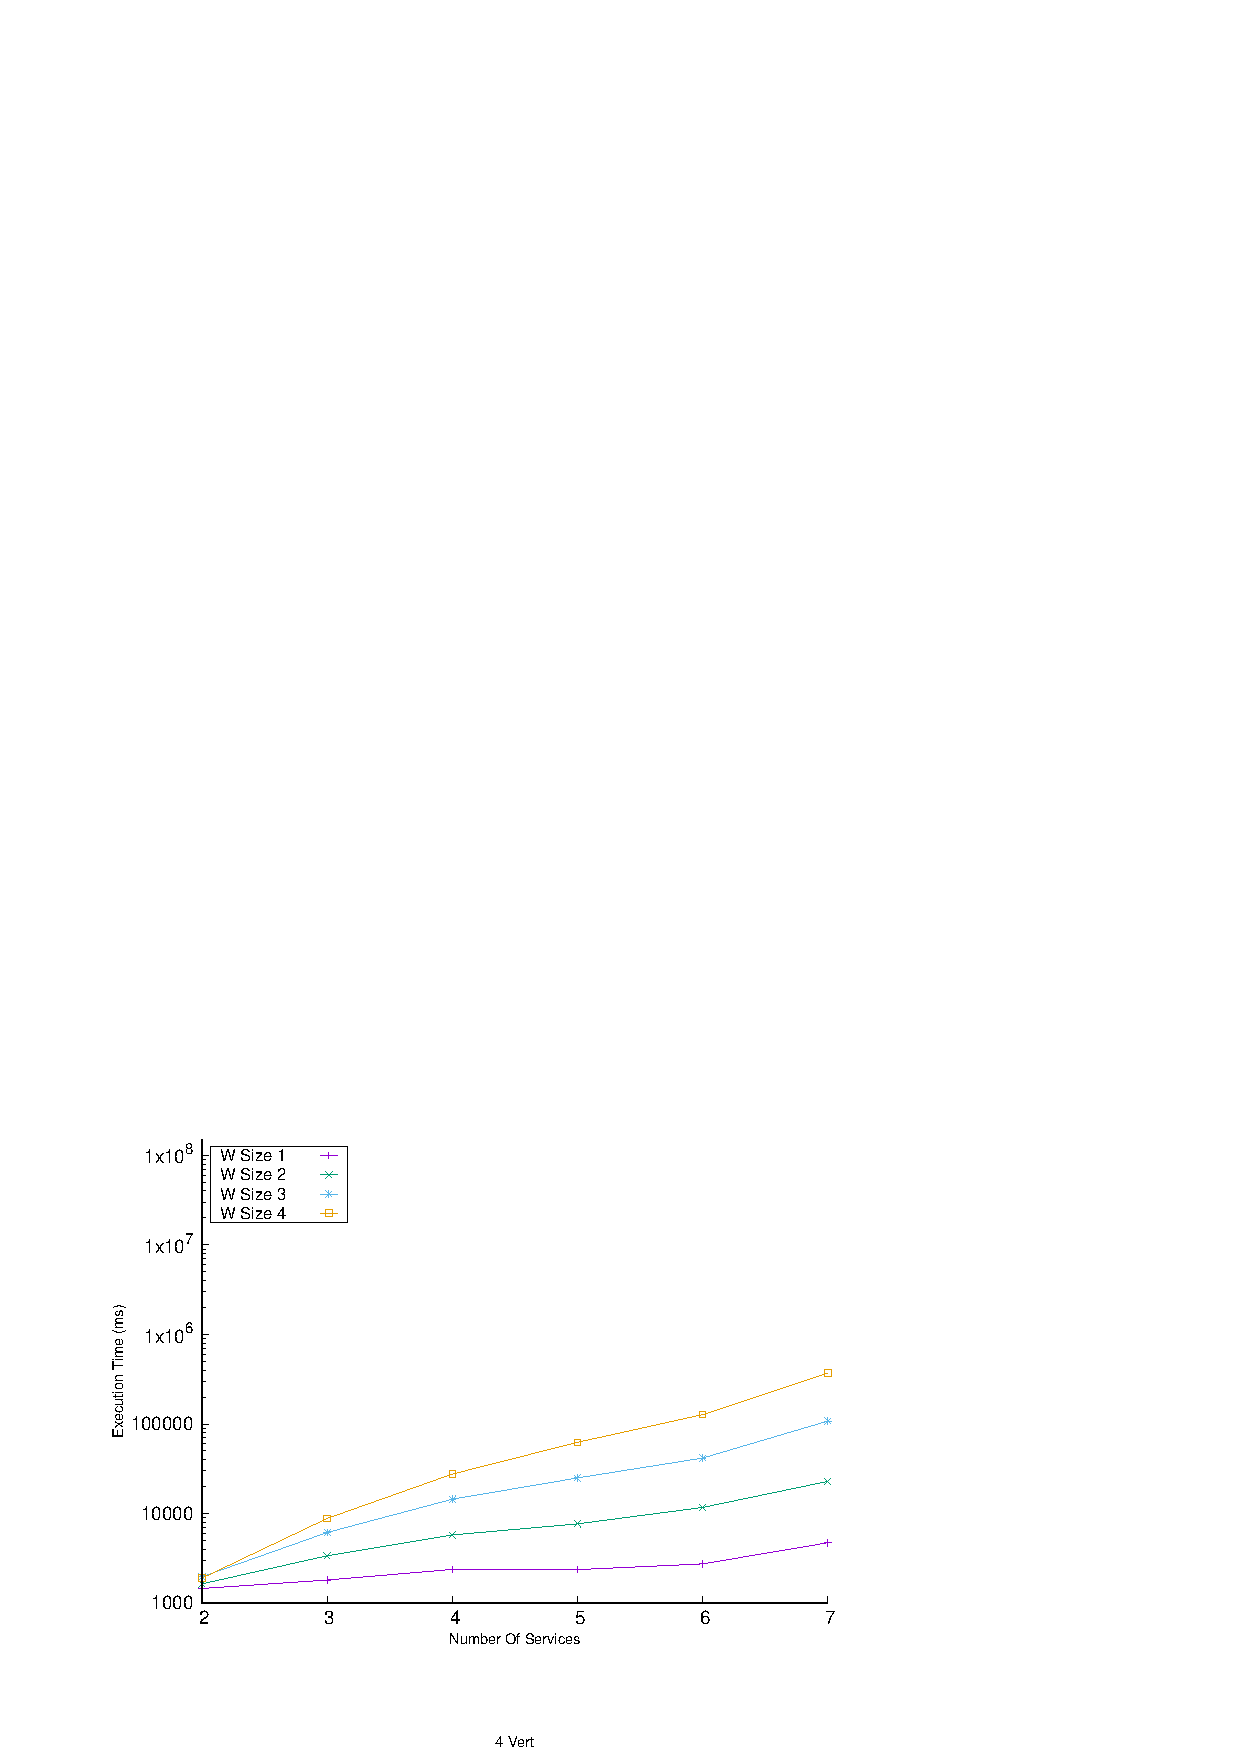
\includegraphics[width=\textwidth]{Images/graphs/window_time_performance_qualitative_n7_s7_50_80_n4}
        \caption{4 vertices}
        \label{fig:time_window_perce_wide_4n}
      \end{subfigure}
      \hfill
      \begin{subfigure}{0.45\textwidth}
        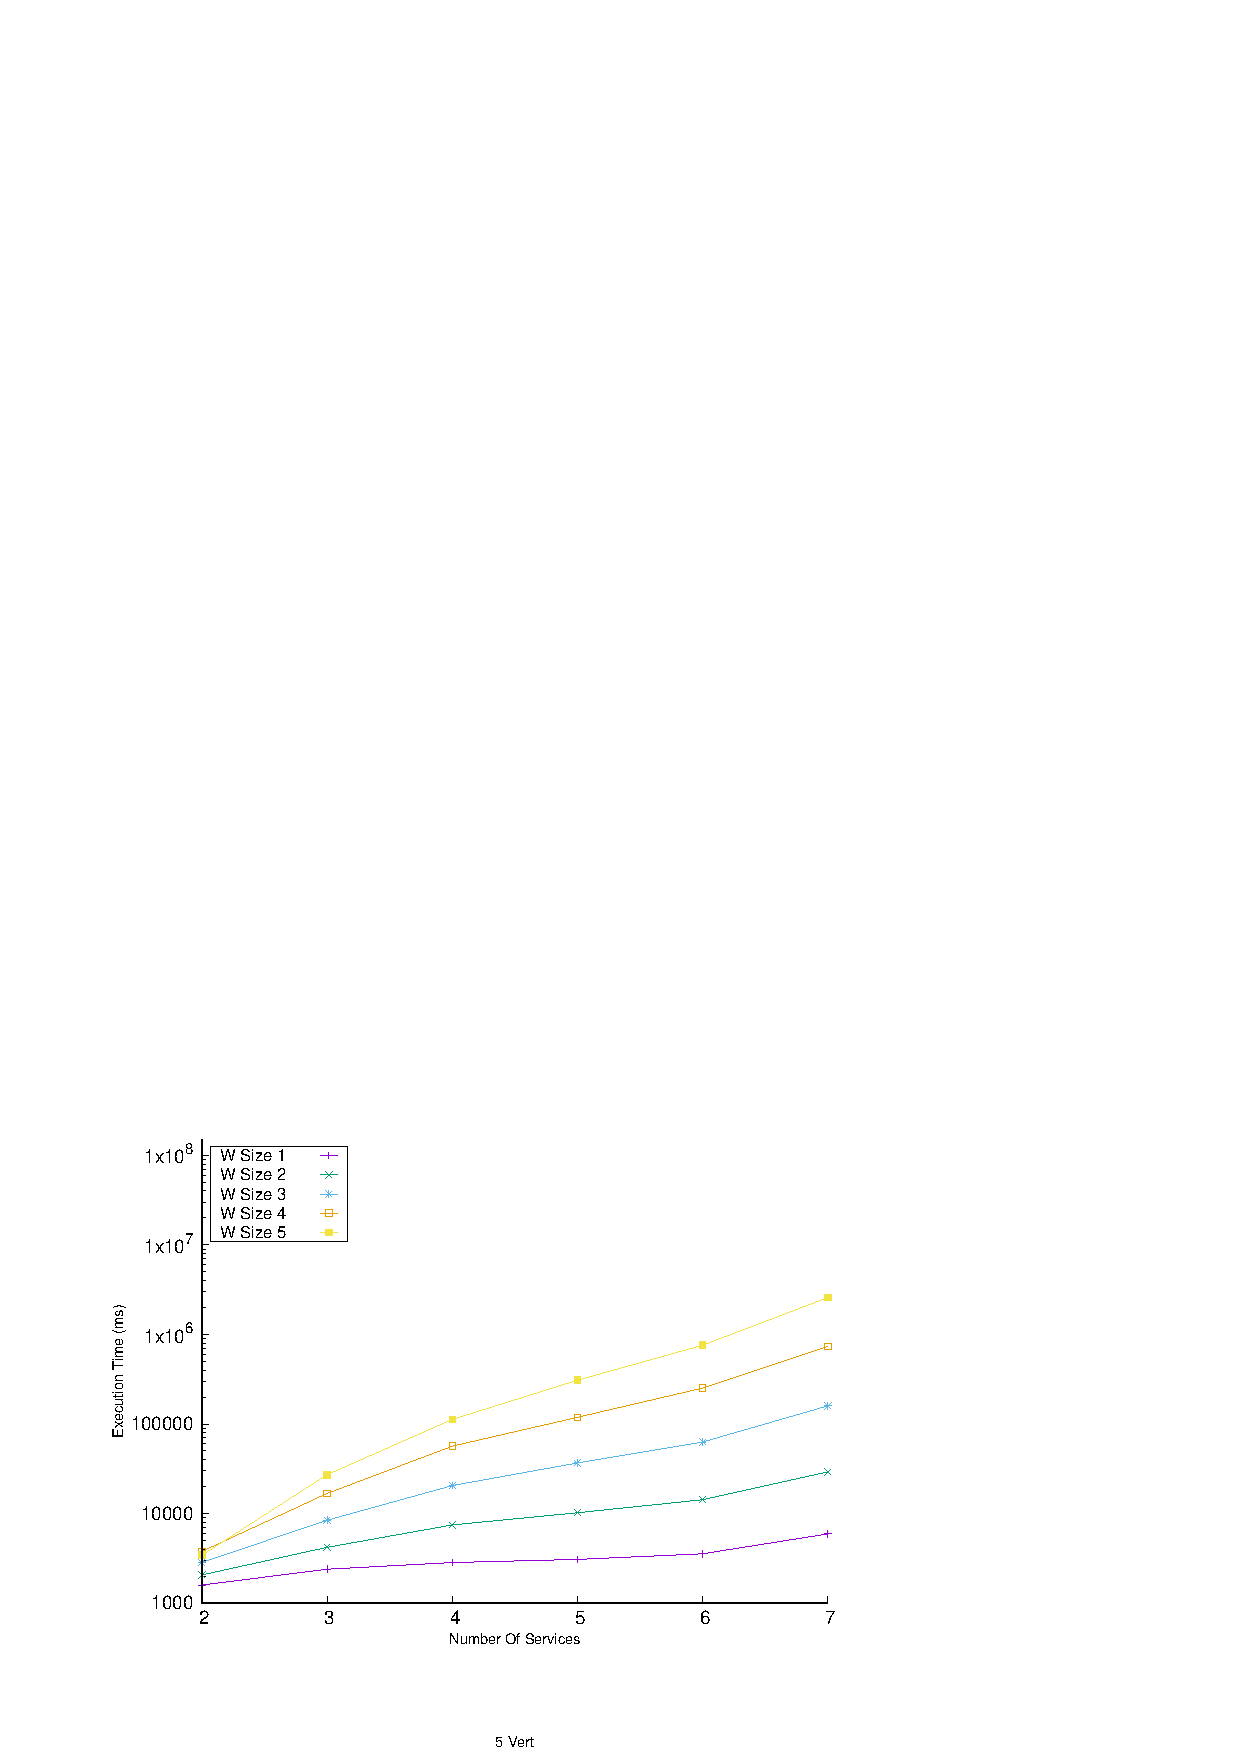
\includegraphics[width=\textwidth]{Images/graphs/window_time_performance_qualitative_n7_s7_50_80_n5}
        \caption{5 vertices}
        \label{fig:time_window_perce_wide_5n}
      \end{subfigure}
      \hfill
      \begin{subfigure}{0.45\textwidth}
        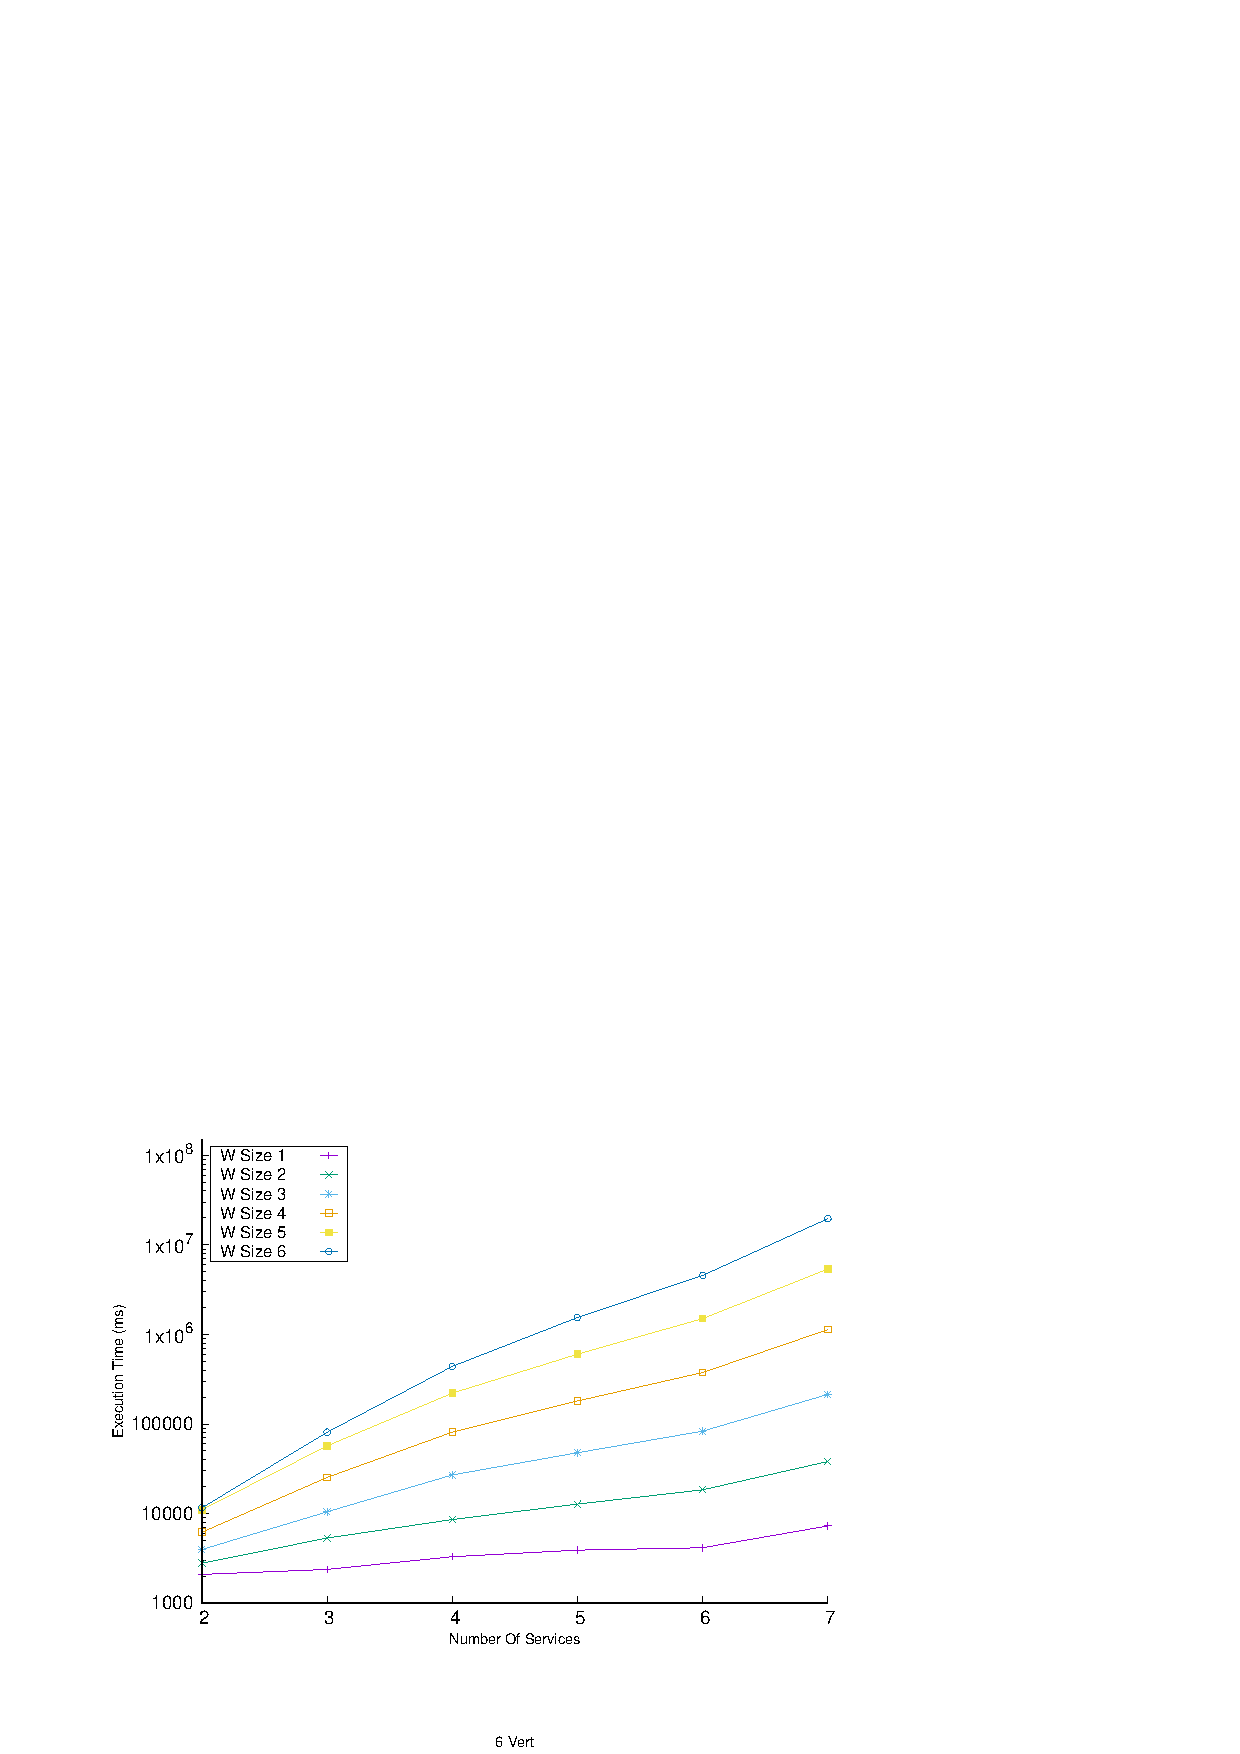
\includegraphics[width=\textwidth]{Images/graphs/window_time_performance_qualitative_n7_s7_50_80_n6}
        \caption{6 vertices}
        \label{fig:time_window_perce_wide_6n}
      \end{subfigure}
      \begin{subfigure}{0.45\textwidth}
        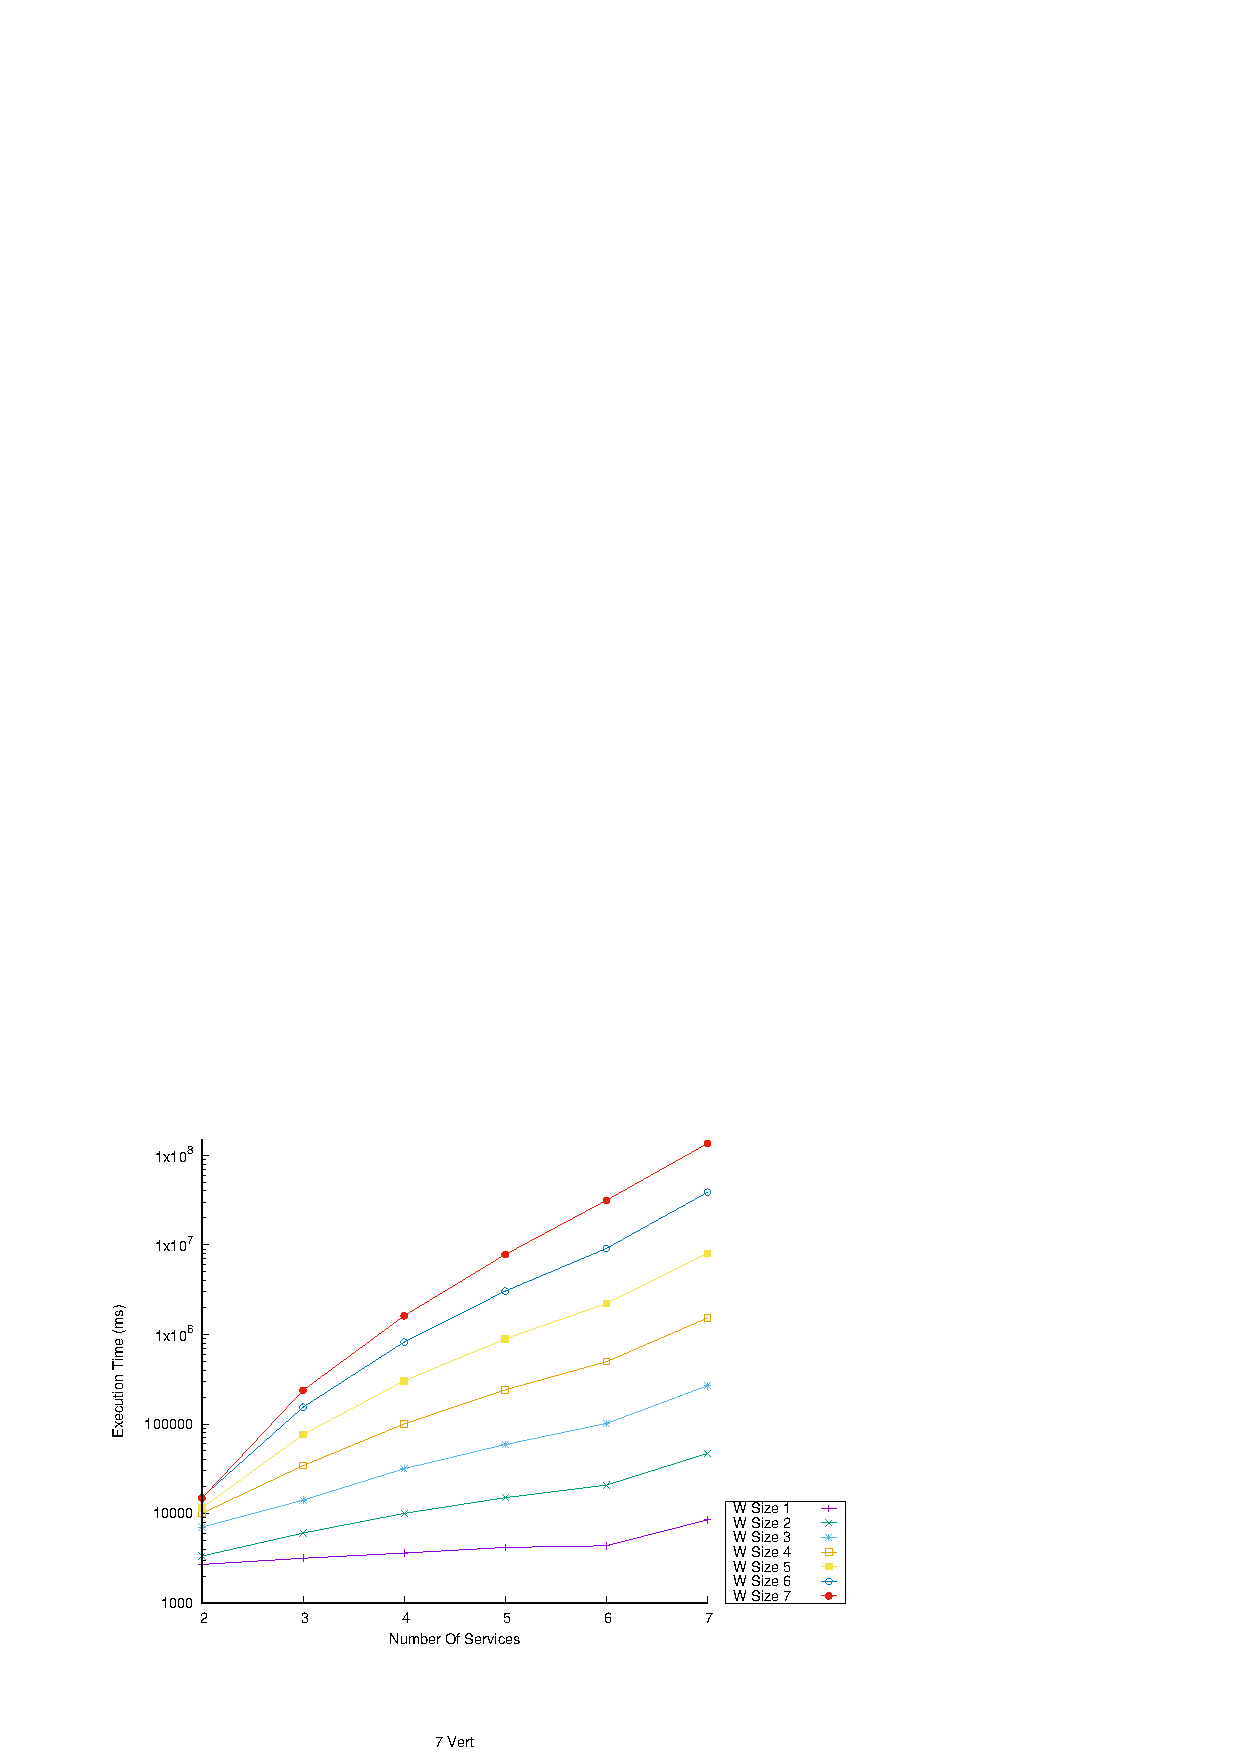
\includegraphics[width=\textwidth]{Images/graphs/window_time_performance_qualitative_n7_s7_50_80_n7}
        \caption{7 vertices}
        \label{fig:time_window_perce_wide_7n}
      \end{subfigure}
      \caption{{\color{OurColor2}Evaluation of Performance Using the \emph{Qualitative} Metric in
            Configuration \average}}
      \label{fig:time_window_perce_average}
    \end{figure}
    \subsection{Performance}\label{subsec:experiments_performance}
    We first measured the performance (execution time) of our exhaustive, baseline, and heuristic solutions by varying the pipeline template length $l$ in [3, 7] and the number of candidate services $|S^c|$ in [2, 7]. \cref{fig:time_window_perce_average} presents our results.
    The exhaustive approach can provide the optimal solution for all settings, but its execution time grows exponentially with the pipeline length and number of candidate services, making it impractical for large instances. For \windowsize\ from 1 to 3 (step 1), we observed a substantial reduction in execution time, with the heuristic always able to produce an instance in less than $\approx2.7\times10^5ms$ . The worst heuristic performance ($l$=7, $|S^c|$=7, \windowsize=6) is $\approx3.8\times10^7ms$, one order of magnitude lower than the best exhaustive performance ($l$=7, $|S^c|$=7, \windowsize=7) $\approx1.35\times10^8ms$. {\color{OurColor} As expected, the baseline (i.e., our heuristic with \windowsize$=$1) shows the best performance in all settings.}


    \subsection{Quality}\label{subsec:experiments_quality}
    We evaluated the quality of our heuristic algorithm with different \windowsize\ comparing its results with the baseline and, where possible, with the optimal solution retrieved by executing the exhaustive approach.
    The quality $Q$ of the heuristic has been normalized between 0 and 1 by dividing it by the quality $Q^*$ retrieved by the exhaustive approach.

    We run our experiments varying: \emph{i)} pipeline template length $l$ in [3, 7], \emph{ii)} the window size \windowsize\ in [1,$l$], and \emph{iii)} the number of candidate services $|S^c|$ in [2, 7]. Each vertex is associated with a (set of) policy that applies filtering configuration \wide (removing a percentage of data in $[0.2,1]$) or \average (removing a percentage of data in $[0.5,0.8]$).

    {\color{OurColor2}\cref{fig:quality_window_perce_average} presents} our quality results using metric $M_J$ in \cref{subsec:metrics} for configurations \wide and \average, respectively.
    In general, we observe that the quality of our heuristic approach increases as the window size increases, providing a quality comparable to the exhaustive approach when the window size \windowsize\ approaches the length $l$ of the pipeline template.

    When considering configuration \wide, the baseline (\windowsize=1) provides good results on average (0.71, 0.90), while showing substantial quality oscillations in specific runs: between 0.882 and 0.970 for pipeline template $l$=3, 0.810 and 0.942 for $l$=4, 0.580 and 0.853 for $l$=5, 0.682 and 0.943 for $l$=6, 0.596 and 0.821 for $l$=7. This same trend emerges when the window size is $<$$l$/2, while it starts approaching the optimum when the window size is $\geq$$l$/2. For instance, when \windowsize=$l$-1, the quality varies between 0.957 and 1.0 for $l$=3, 0.982 and 1.0 for $l$=4, 0.986 and 0.998 for $l$=5, 0.977 and 1.0 for $l$=6, 0.996 and 1.0 for $l$=7.
    \begin{figure}[ht]
      \centering
      \begin{subfigure}{0.49\textwidth}
        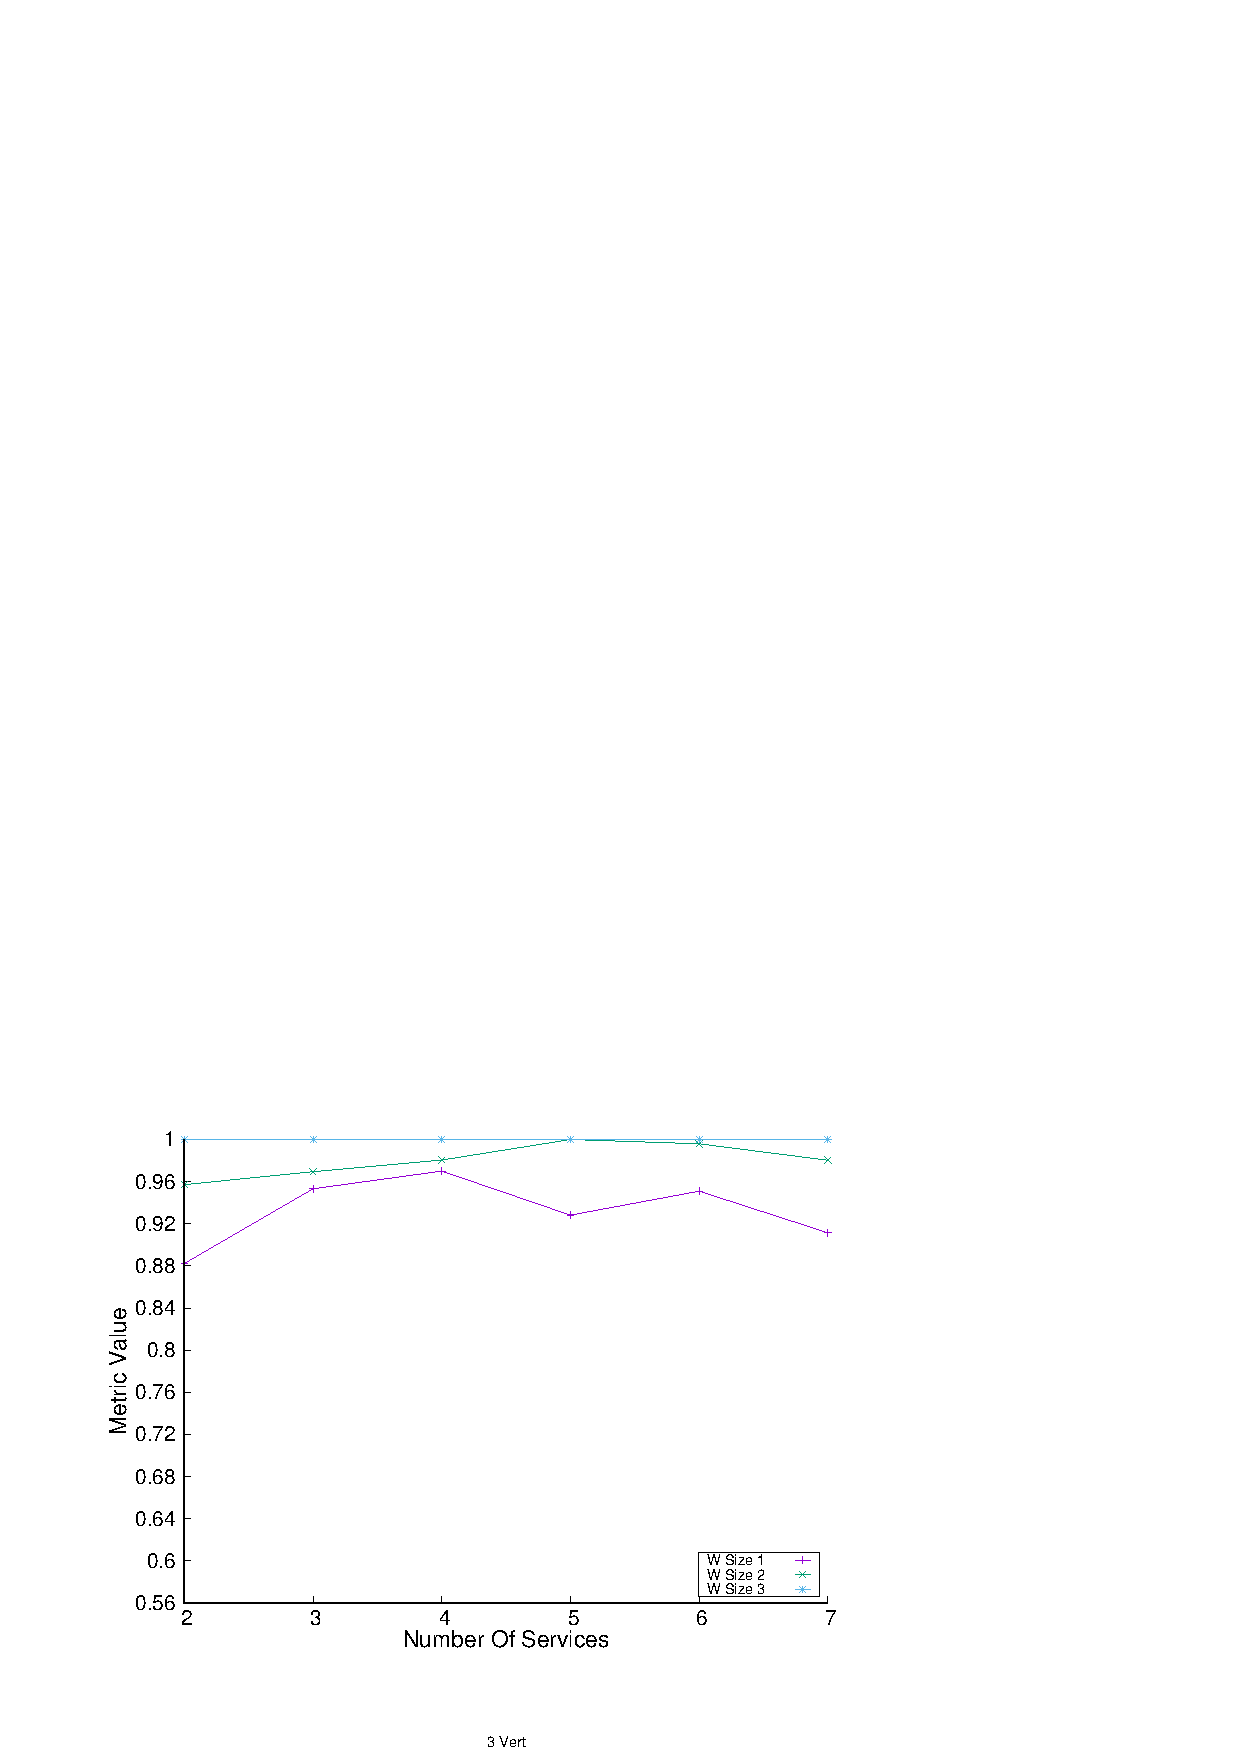
\includegraphics[width=\textwidth]{Images/graphs/window_quality_performance_diff_perce_n7_s7_20_100_n3}
        \caption{\wide 3 vertices}
        \label{fig:quality_window_wide_perce_n3}
      \end{subfigure}
      \hfill
      \begin{subfigure}{0.49\textwidth}
        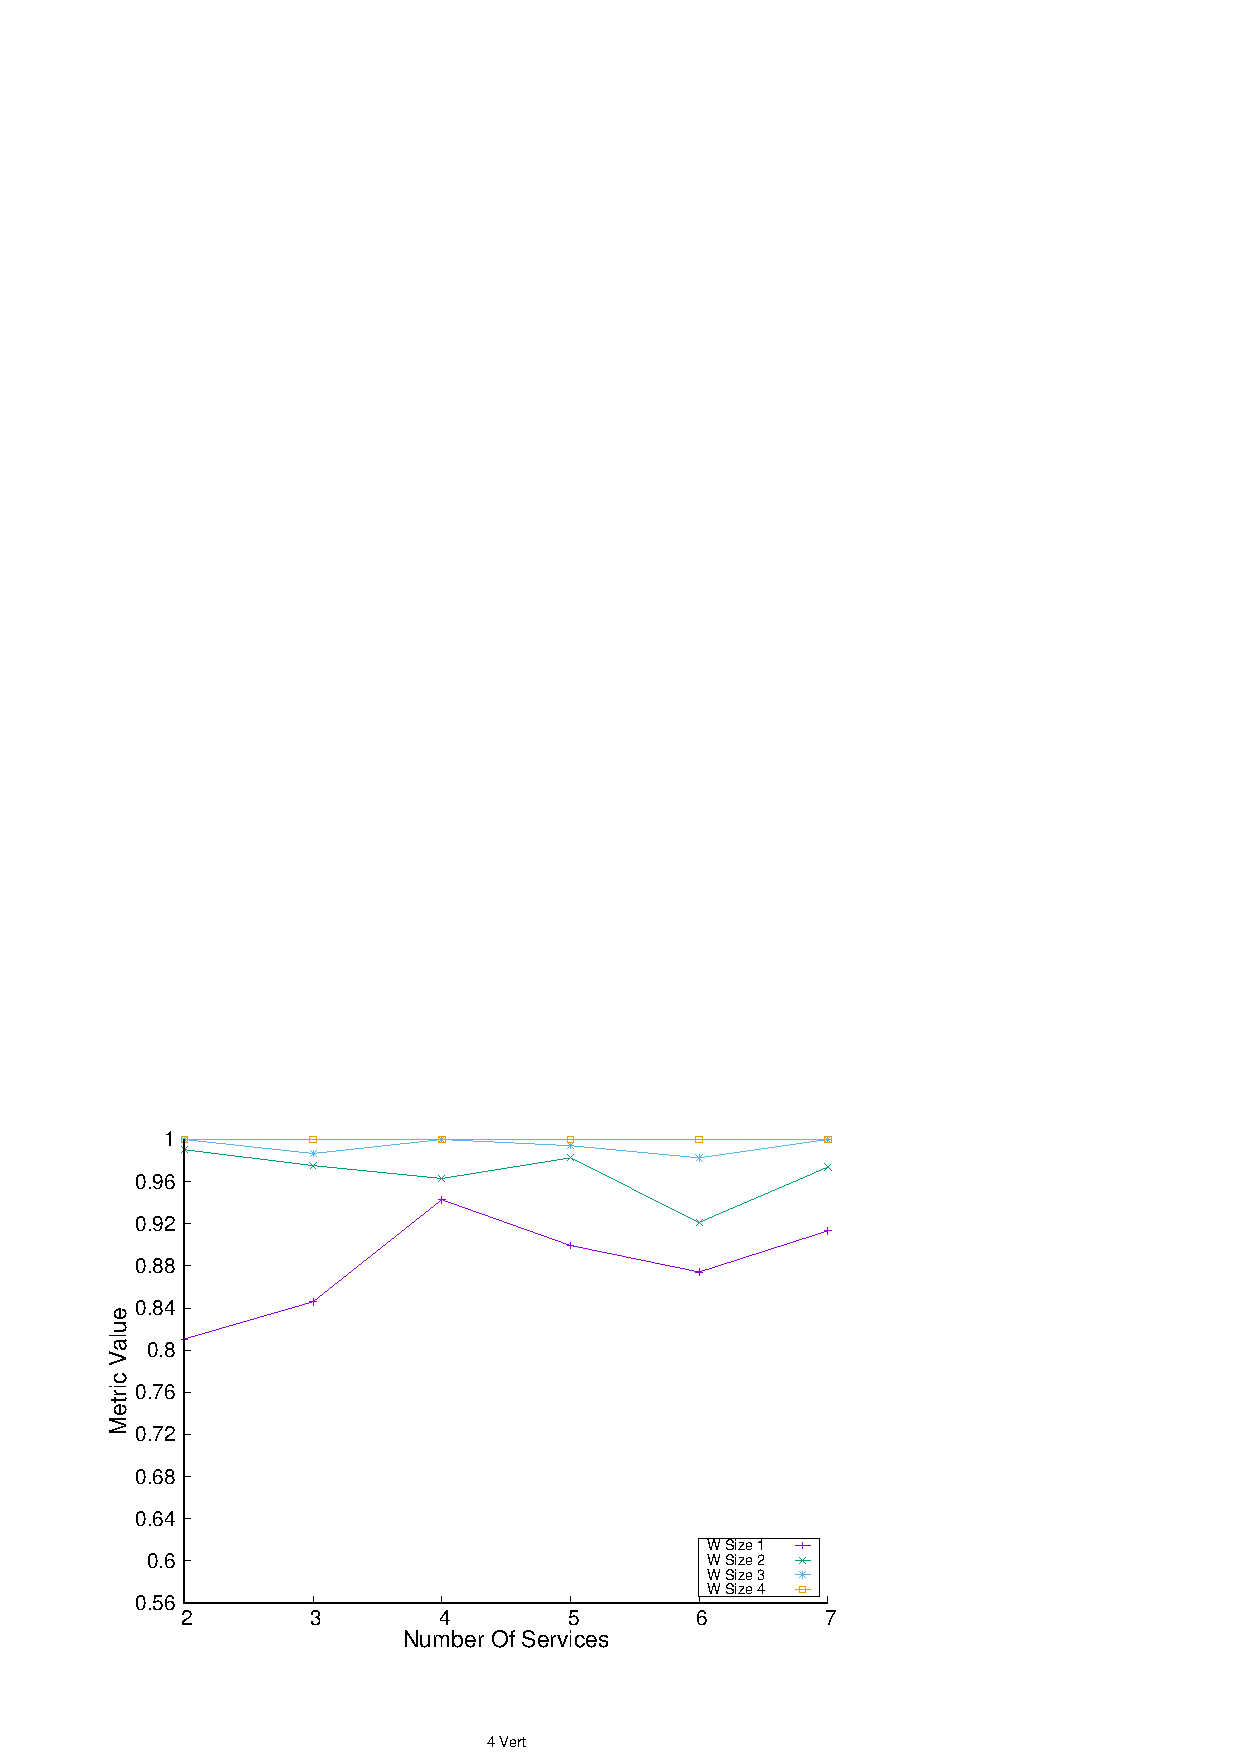
\includegraphics[width=\textwidth]{Images/graphs/window_quality_performance_diff_perce_n7_s7_20_100_n4}
        \caption{\wide 4 vertices}
        \label{fig:quality_window_wide_perce_n4}
      \end{subfigure}
      \hfill
      \begin{subfigure}{0.49\textwidth}
        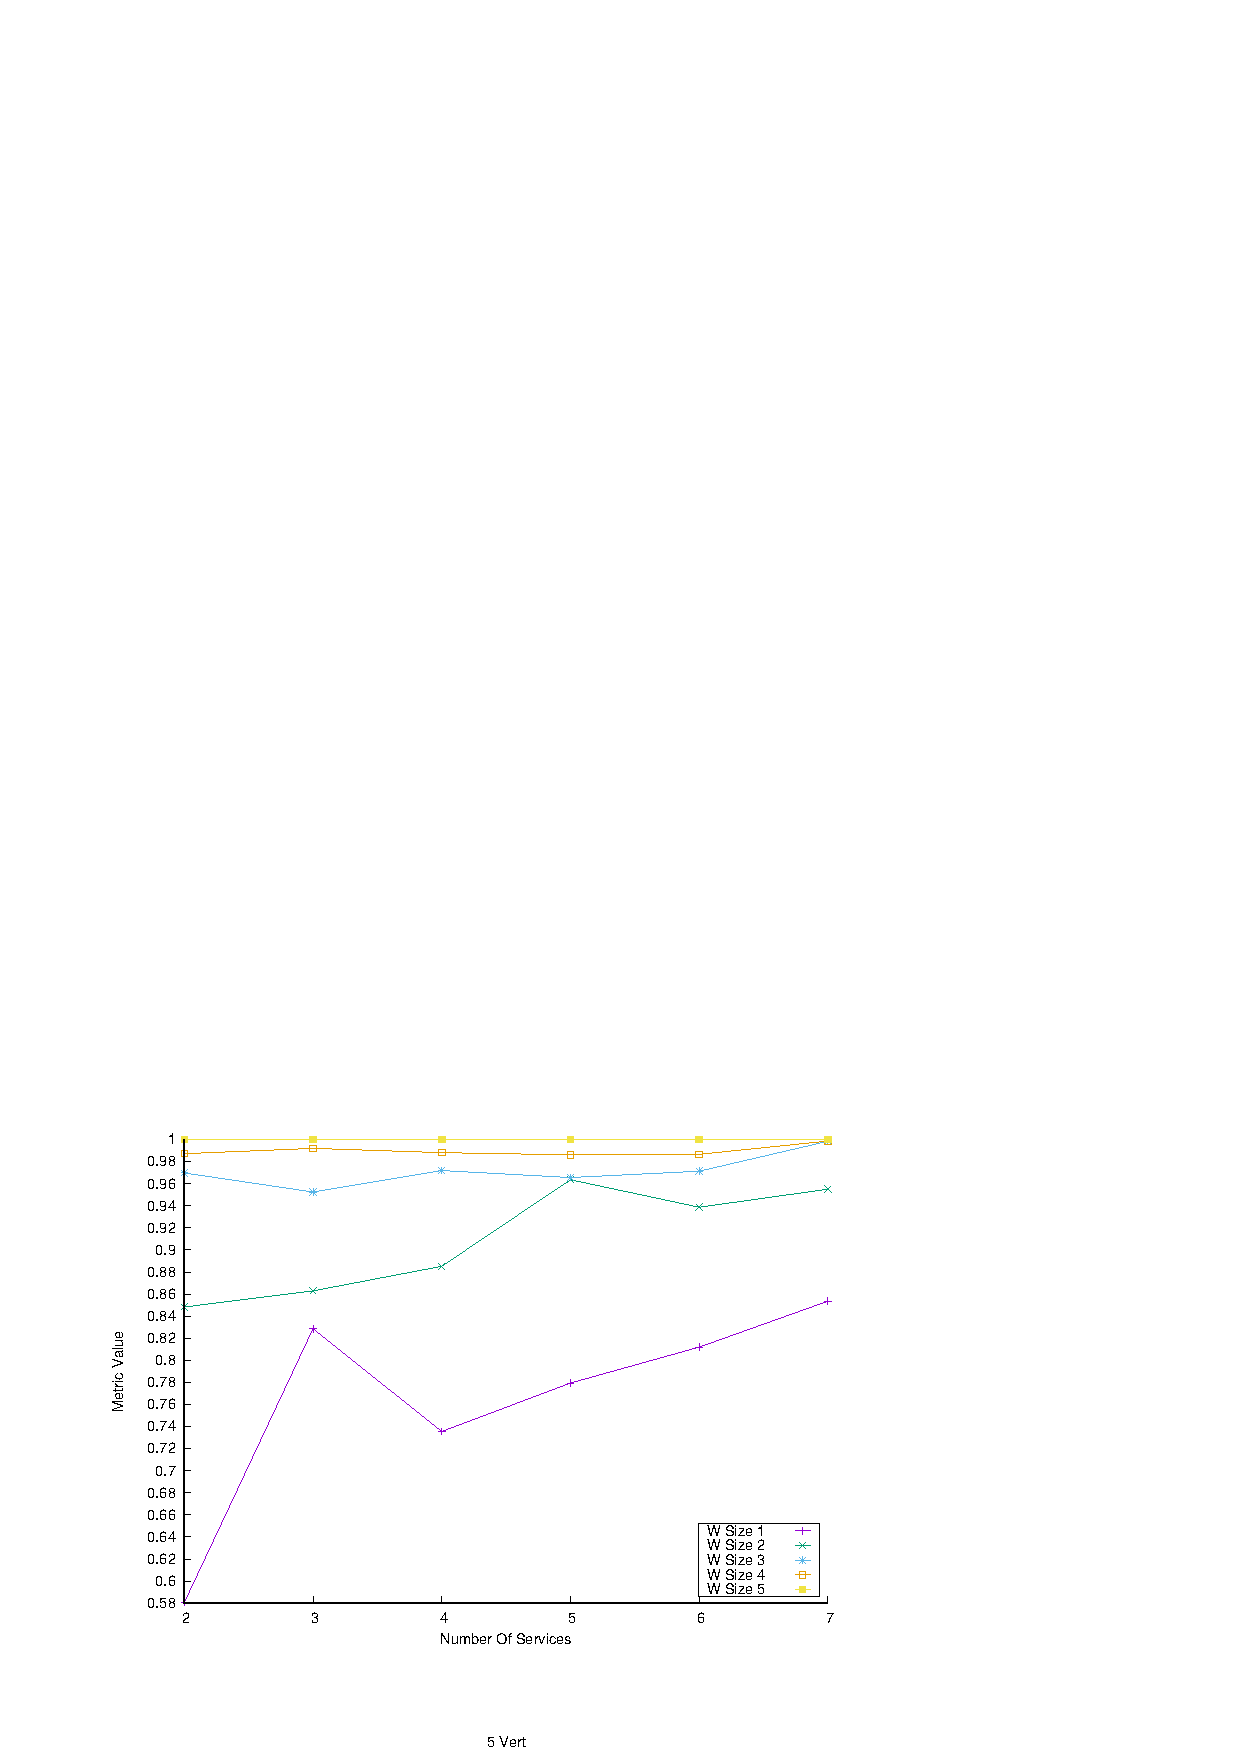
\includegraphics[width=\textwidth]{Images/graphs/window_quality_performance_diff_perce_n7_s7_20_100_n5}
        \caption{\wide 5 vertices}

        \label{fig:quality_window_wide_perce_n5}
      \end{subfigure}
      \hfill
      \begin{subfigure}{0.49\textwidth}
        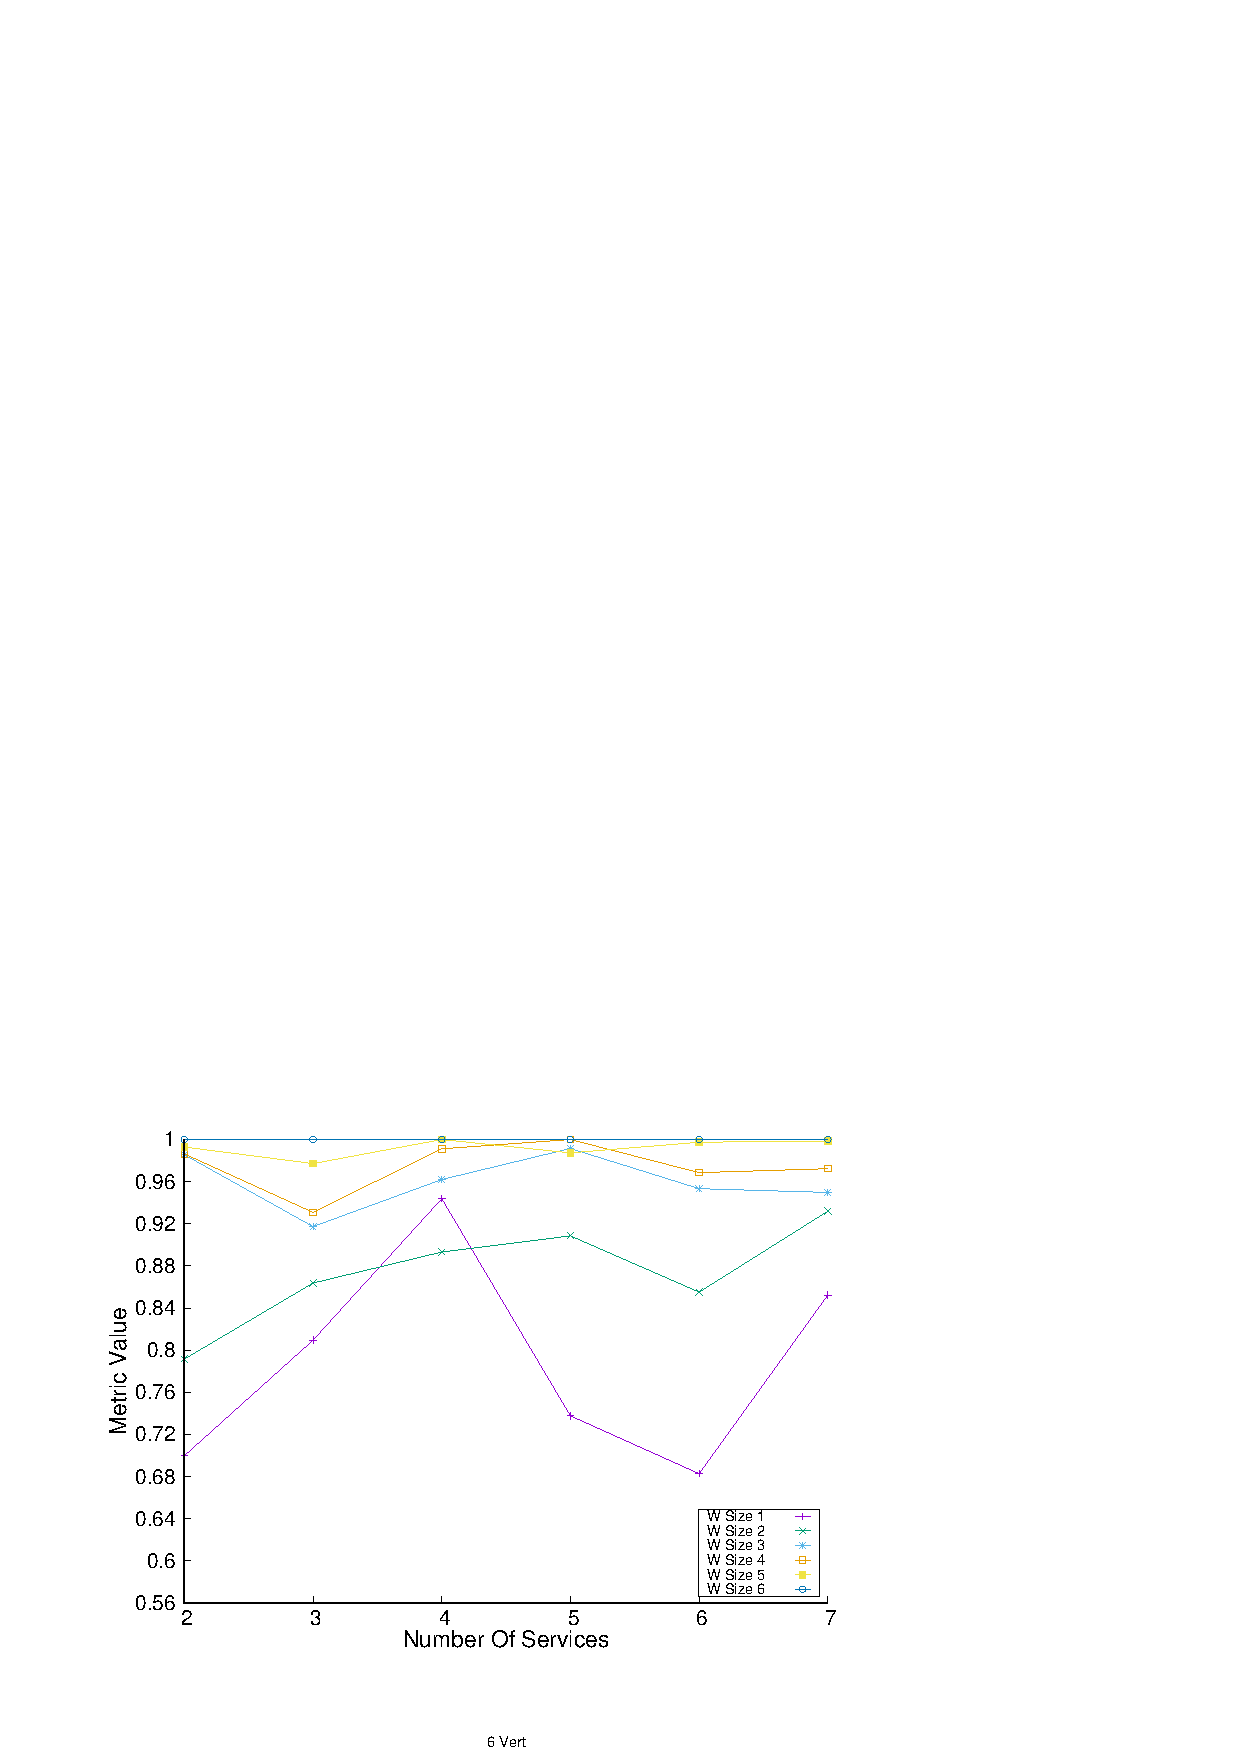
\includegraphics[width=\textwidth]{Images/graphs/window_quality_performance_diff_perce_n7_s7_20_100_n6}
        \caption{\wide 6 vertices}
        \label{fig:quality_window_wide_perce_n6}
      \end{subfigure}
      \hfill
      \begin{subfigure}{0.49\textwidth}
        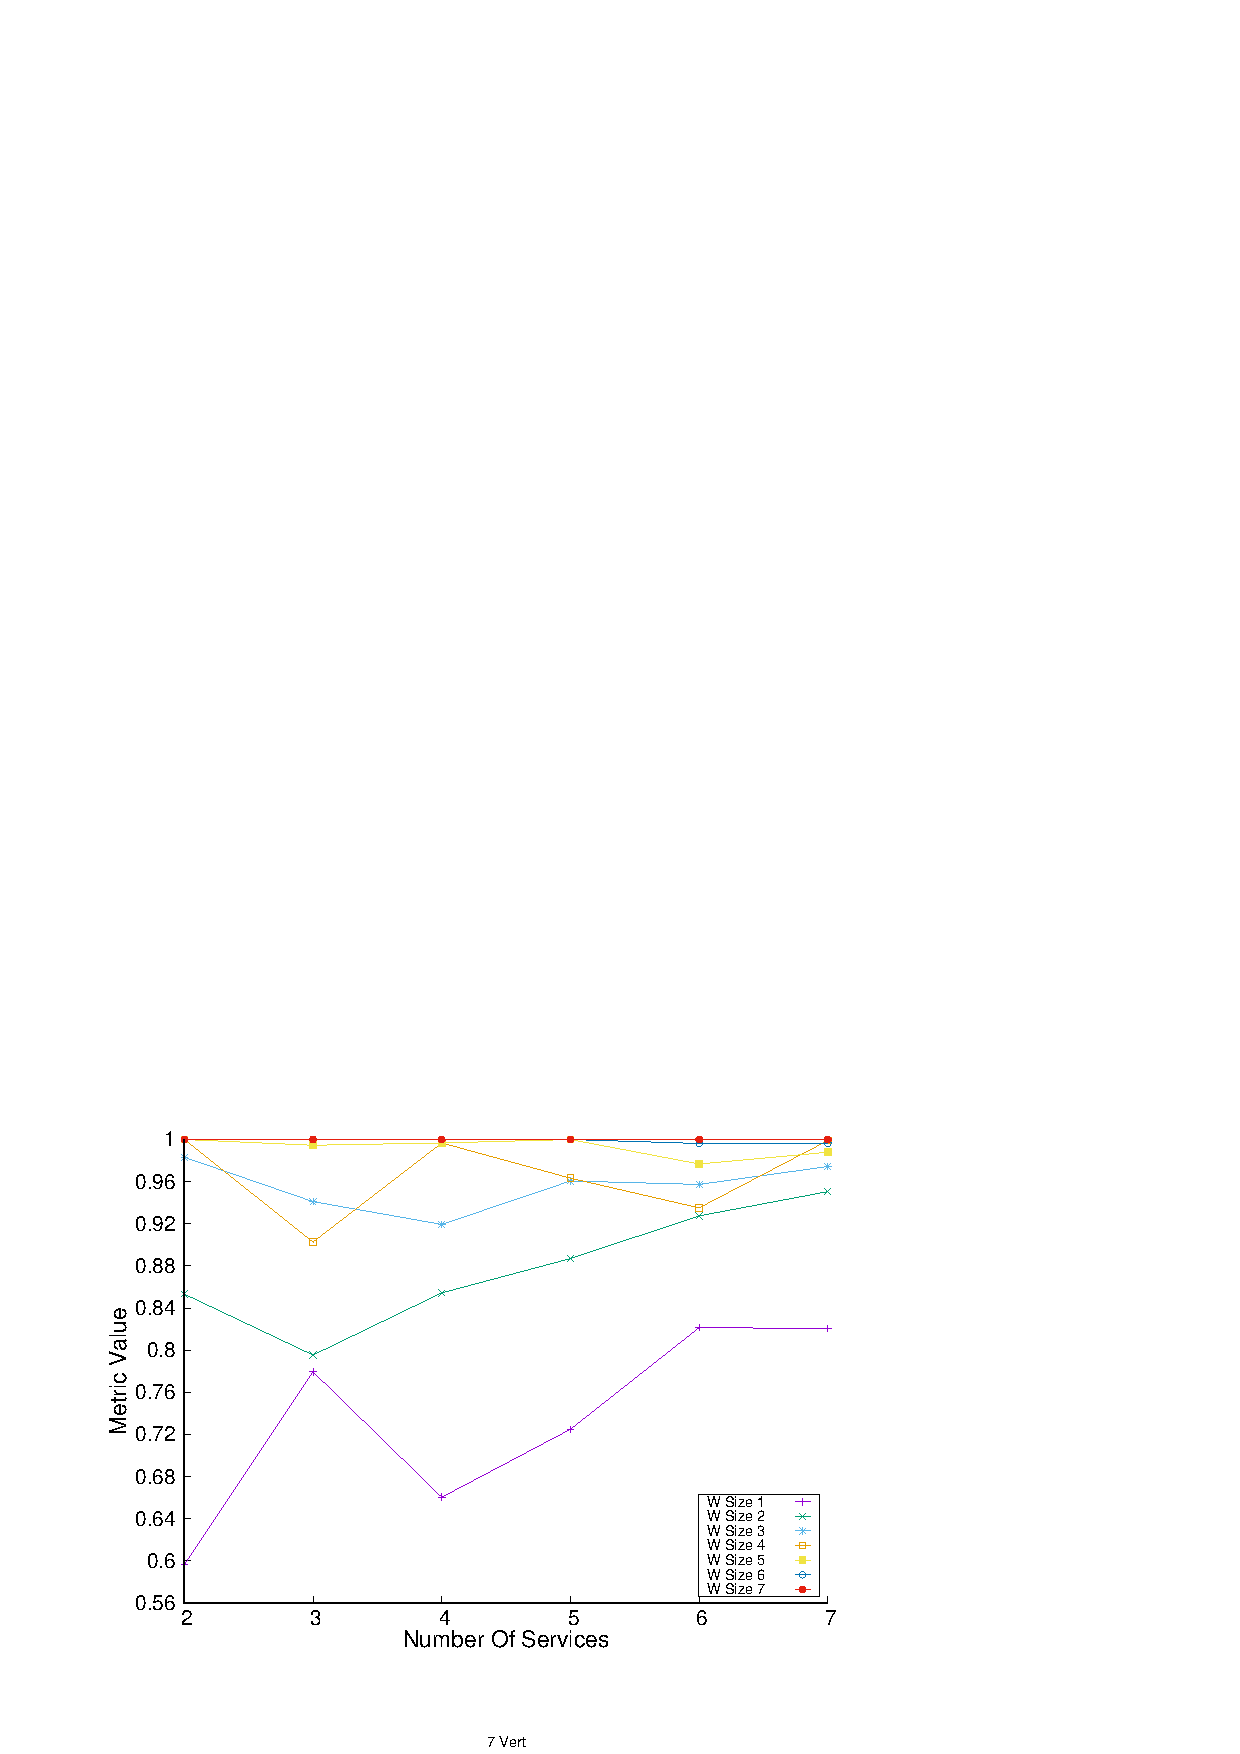
\includegraphics[width=\textwidth]{Images/graphs/window_quality_performance_diff_perce_n7_s7_20_100_n7}
        \caption{\wide 7 vertices}
        \label{fig:quality_window_wide_perce_n7}
      \end{subfigure}



      \caption{Evaluation of Quality Using the \emph{Quantitative} Metric in a \wide (\cref{fig:quality_window_wide_perce_n3,fig:quality_window_wide_perce_n4,fig:quality_window_wide_perce_n5,fig:quality_window_wide_perce_n6,fig:quality_window_wide_perce_n7}) Profile Configuration.}  \label{fig:quality_window_perce_wide}

    \end{figure}



    When considering configuration \average (\cref{fig:quality_window_perce_average}), the heuristic algorithm still provides good results, limiting the quality oscillations observed for configuration \wide\ and approaching the quality of the exhaustive also for lower window sizes. The baseline (\windowsize=1) provides good results on average (from 0.842 to 0.944), as well as in specific runs: between 0.927 and 0.978 for $l$=3, 0.903 and 0.962 for $l$=4, 0.840 and 0.915 for $l$=5, 0.815 and 0.934 for $l$=6, 0.721 and 0.935 for $l$=7.
    When \windowsize=$l$-1, the quality varies between 0.980 and 1.0 for $l$=3, 0.978 and 1.0 for $l$=4, 0.954 and 1 for $l$=5, 0.987 and 1.0 for $l$=6, 0.990 and 1.0 for $l$=7.

    \cref{fig:quality_window_perce_average,fig:quality_window_perce_wide} {\color{OurColor2}presents} our quality results using metric $M_{JSD}$ in \cref{subsec:metrics} for configurations \wide and \average, respectively.
    \begin{figure}[ht]
      \centering
      \begin{subfigure}{0.49\textwidth}
        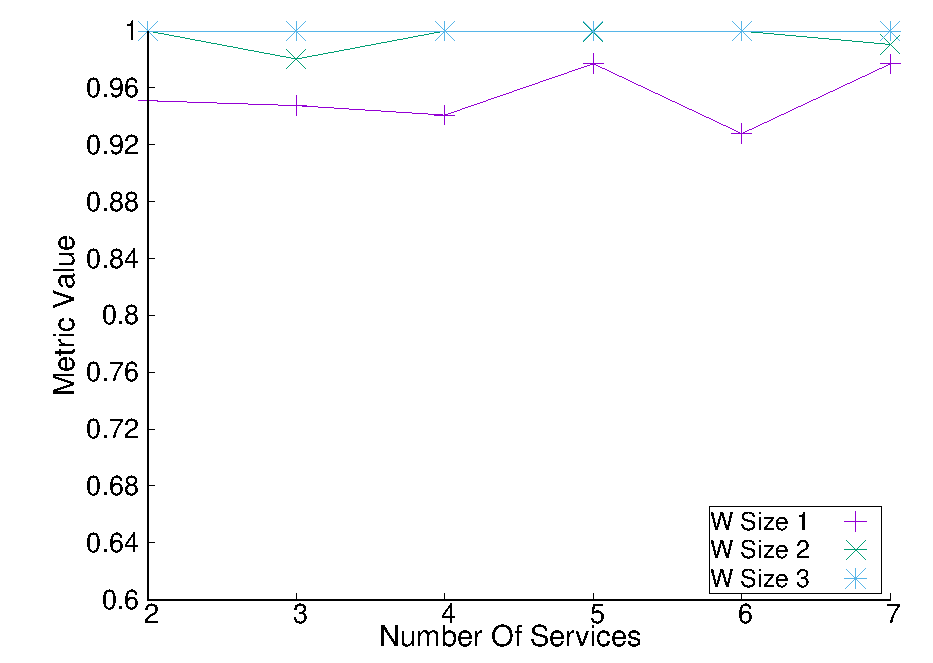
\includegraphics[width=\textwidth]{Images/graphs/window_quality_performance_diff_perce_n7_s7_50_89_n3}
        \caption{\average 3 vertices}

        \label{fig:quality_window_average_perce_n3}
      \end{subfigure}
      \hfill
      \begin{subfigure}{0.49\textwidth}
        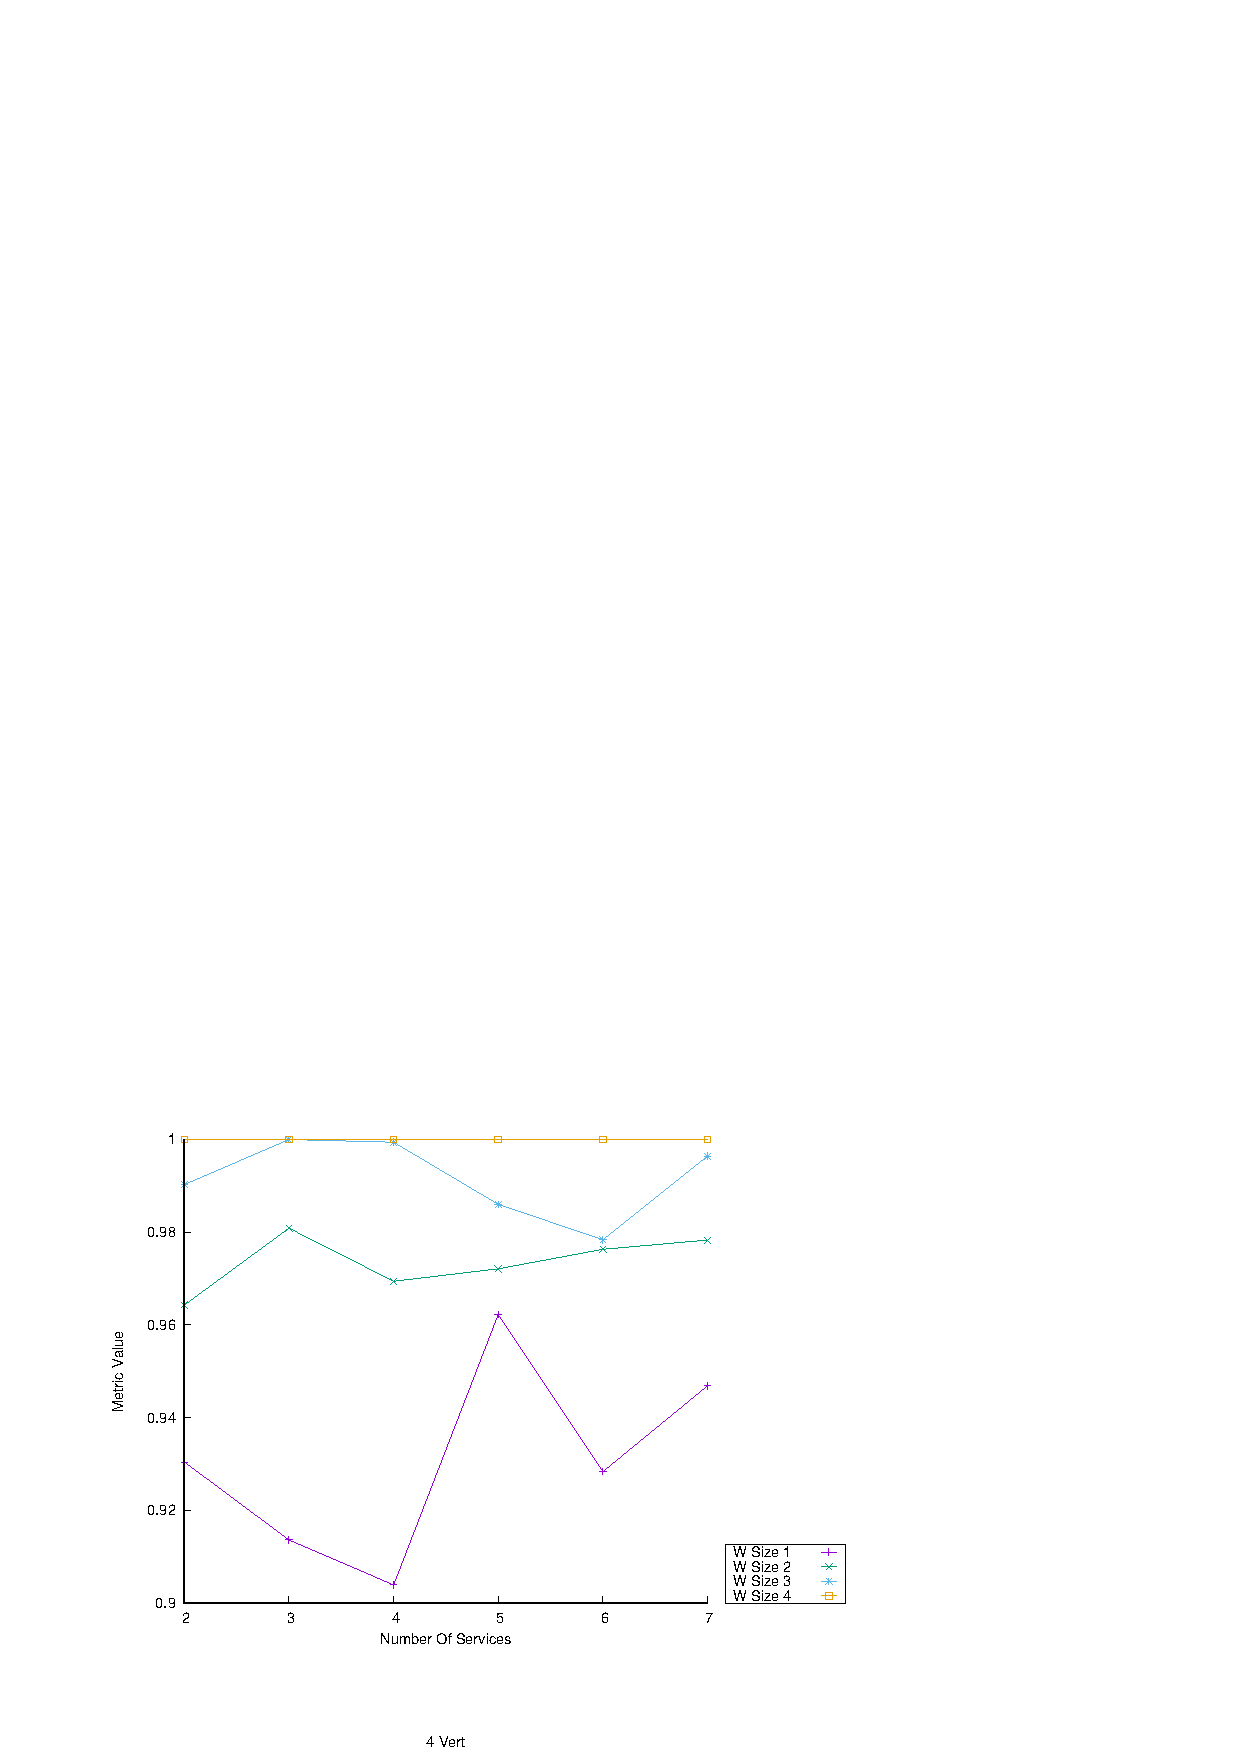
\includegraphics[width=\textwidth]{Images/graphs/window_quality_performance_diff_perce_n7_s7_50_89_n4}
        \caption{\average 4 vertices}

        \label{fig:quality_window_average_perce_n4}
      \end{subfigure}
      \hfill
      \begin{subfigure}{0.49\textwidth}
        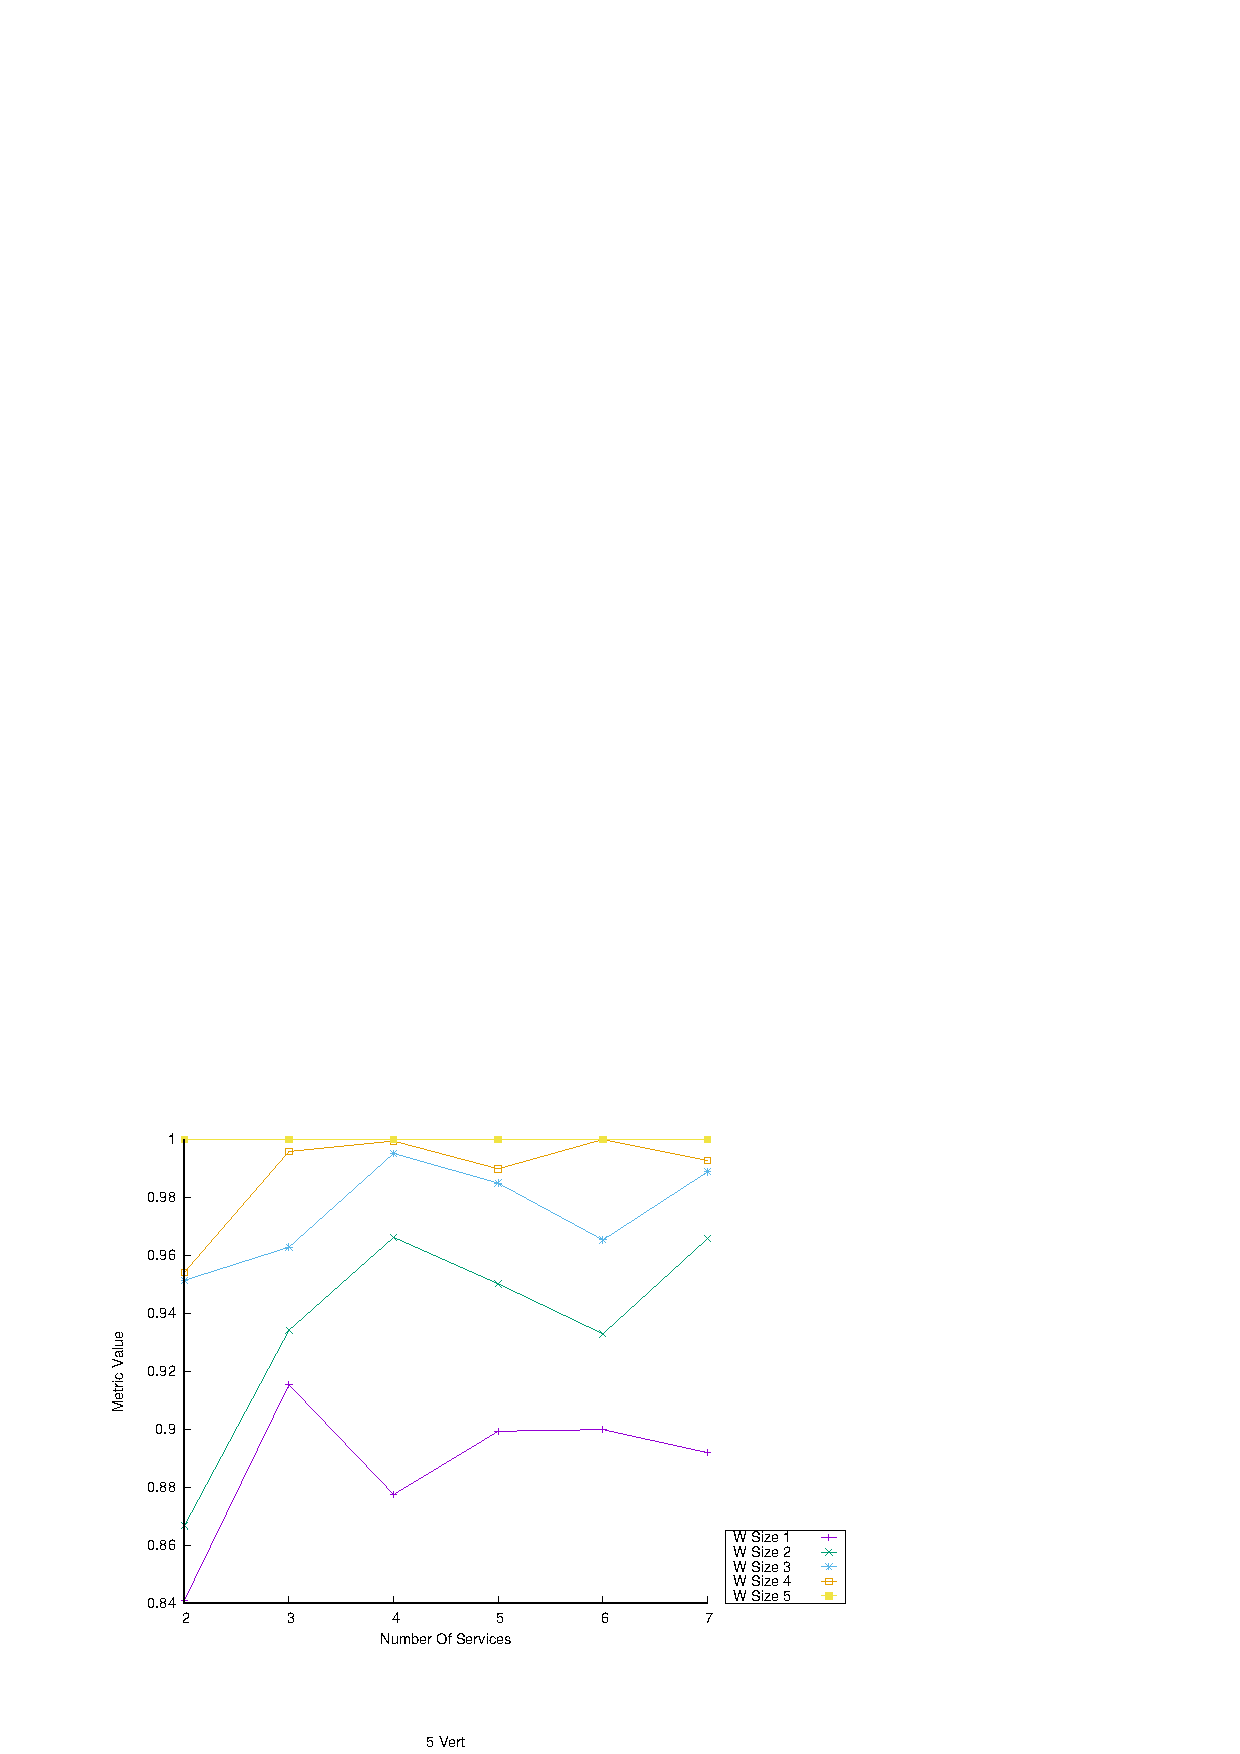
\includegraphics[width=\textwidth]{Images/graphs/window_quality_performance_diff_perce_n7_s7_50_89_n5}
        \caption{\average 5 vertices}
        \label{fig:quality_window_average_perce_n5}
      \end{subfigure}
      \hfill
      \begin{subfigure}{0.49\textwidth}
        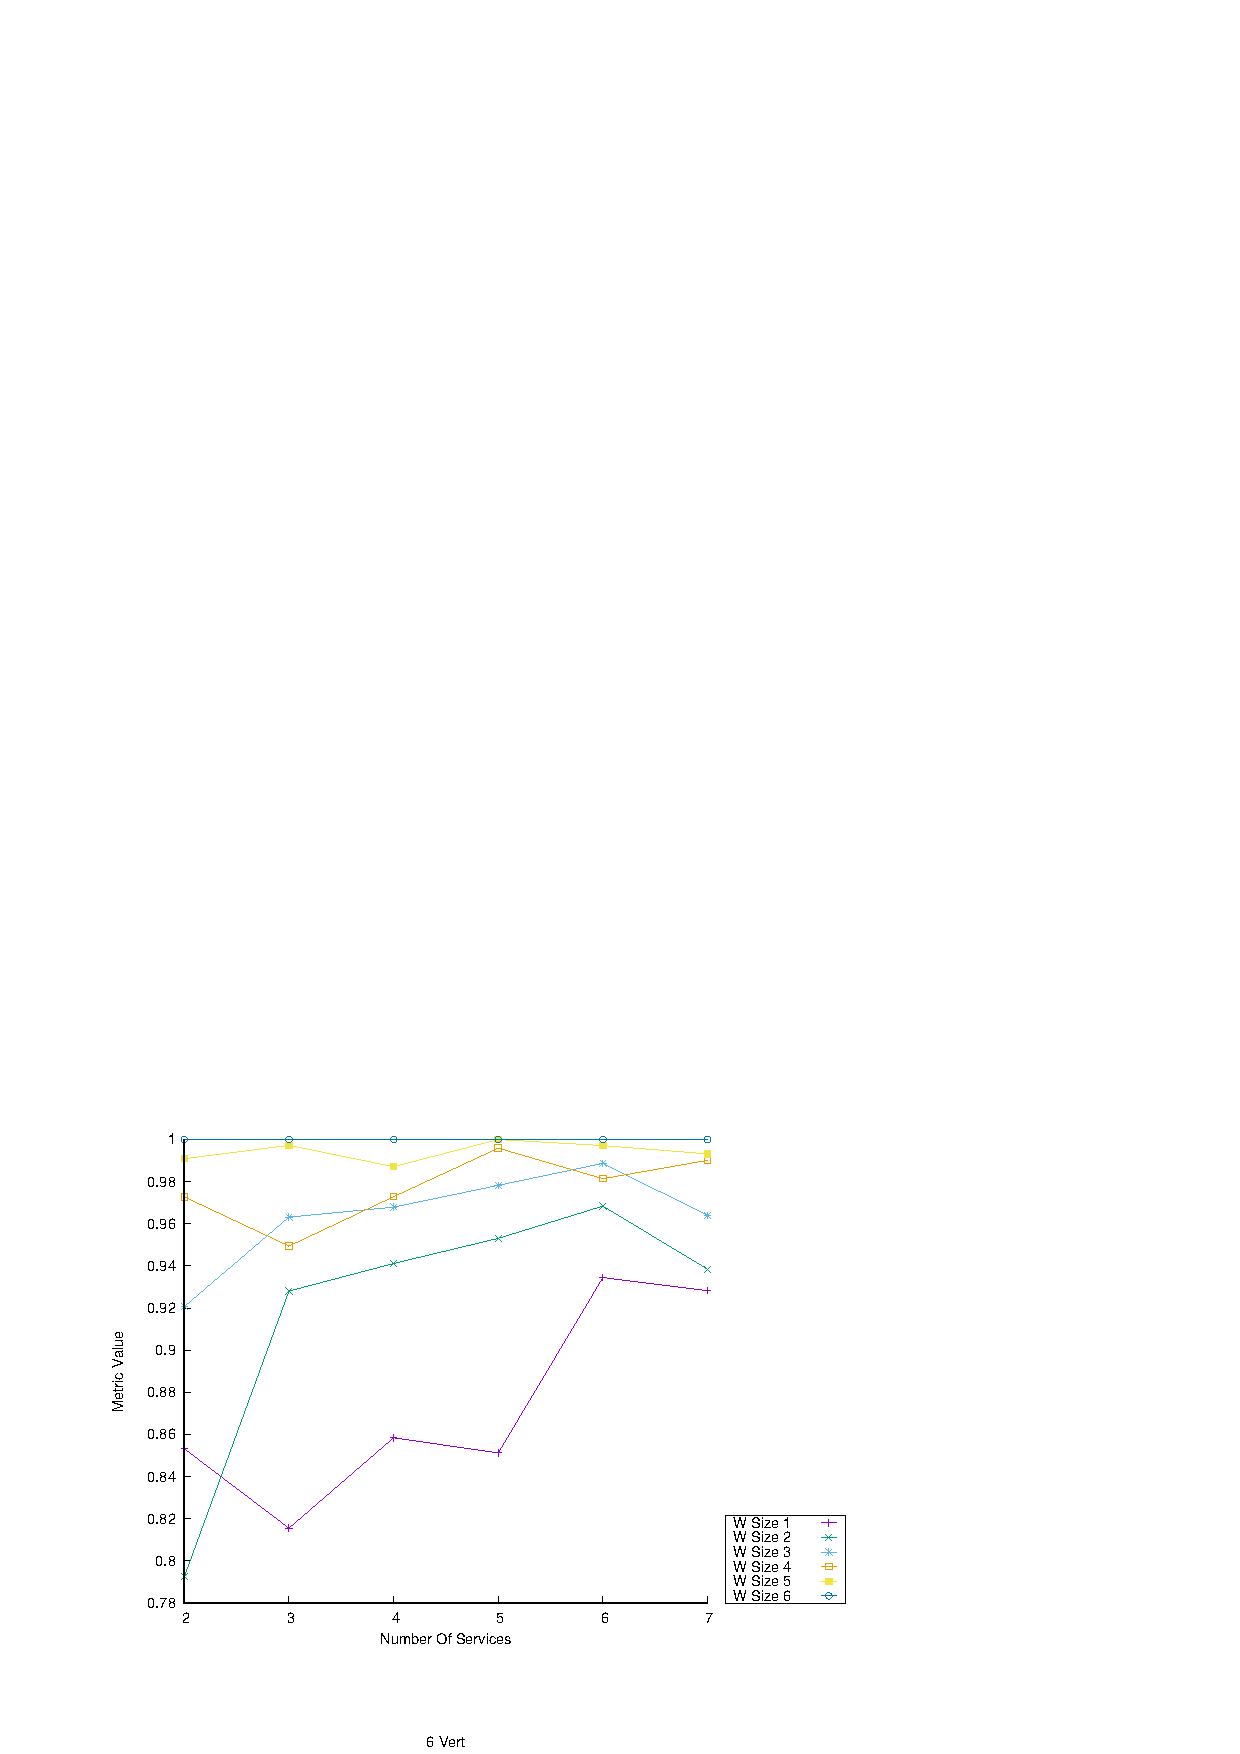
\includegraphics[width=\textwidth]{Images/graphs/window_quality_performance_diff_perce_n7_s7_50_89_n6}
        \caption{\average 6 vertices}
        \label{fig:quality_window_average_perce_n6}
      \end{subfigure}
      \hfill
      \begin{subfigure}{0.49\textwidth}
        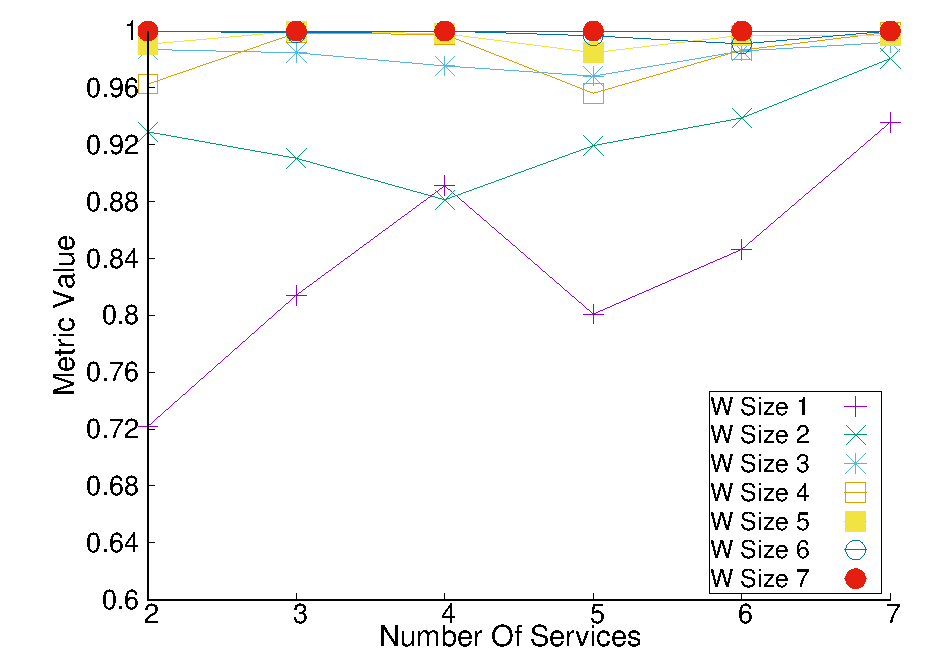
\includegraphics[width=\textwidth]{Images/graphs/window_quality_performance_diff_perce_n7_s7_50_89_n7}
        \caption{\average 7 vertices}
        \label{fig:quality_window_average_perce_n7}
      \end{subfigure}


      \caption{Evaluation of Quality Using the \emph{Quantitative} Metric in an \average (\cref{fig:quality_window_average_perce_n3,fig:quality_window_average_perce_n4,fig:quality_window_average_perce_n5,fig:quality_window_average_perce_n6,fig:quality_window_average_perce_n7}) Profile Configuration.}  \label{fig:quality_window_perce_average}

    \end{figure}

    %QUAAAAAAAAAAAAAAAAAAAA

    When considering configuration \wide, the baseline (\windowsize=1) provides good results on average (0.92, 0.97), limiting oscillations observed with metric $M_J$; for instance, the quality varies between 0.951 and 0.989 for $l$=3, 0.941 and 0.988 for $l$=4, 0.919 and 0.974 for $l$=5, 0.911 and 0.971 for $l$=6, 0.877 and 0.924 for $l$=7.
    The worst quality results are obtained with the baseline, while the oscillations are negligible when the window size is $>$2. For instance, when \windowsize=$l$-2, the quality varies between, 0.982 and 0.996 for $l$=4, 0.981 and 0.998 for $l$=5, 0.988 and 1.0 for $l$=6, 0.976 and 0.999 for $l$=7. When \windowsize=$l$-1, the quality varies between  0.987 and  0.998 for $l$=3, 0.993 and 1.0 for $l$=4, 0.985 and 0.999 for $l$=5, 0.997 and 1.0 for $l$=6, 0.995 and 1.0  for $l$=7.

    \begin{figure}[H]
      \centering
      \begin{subfigure}{0.49\textwidth}
        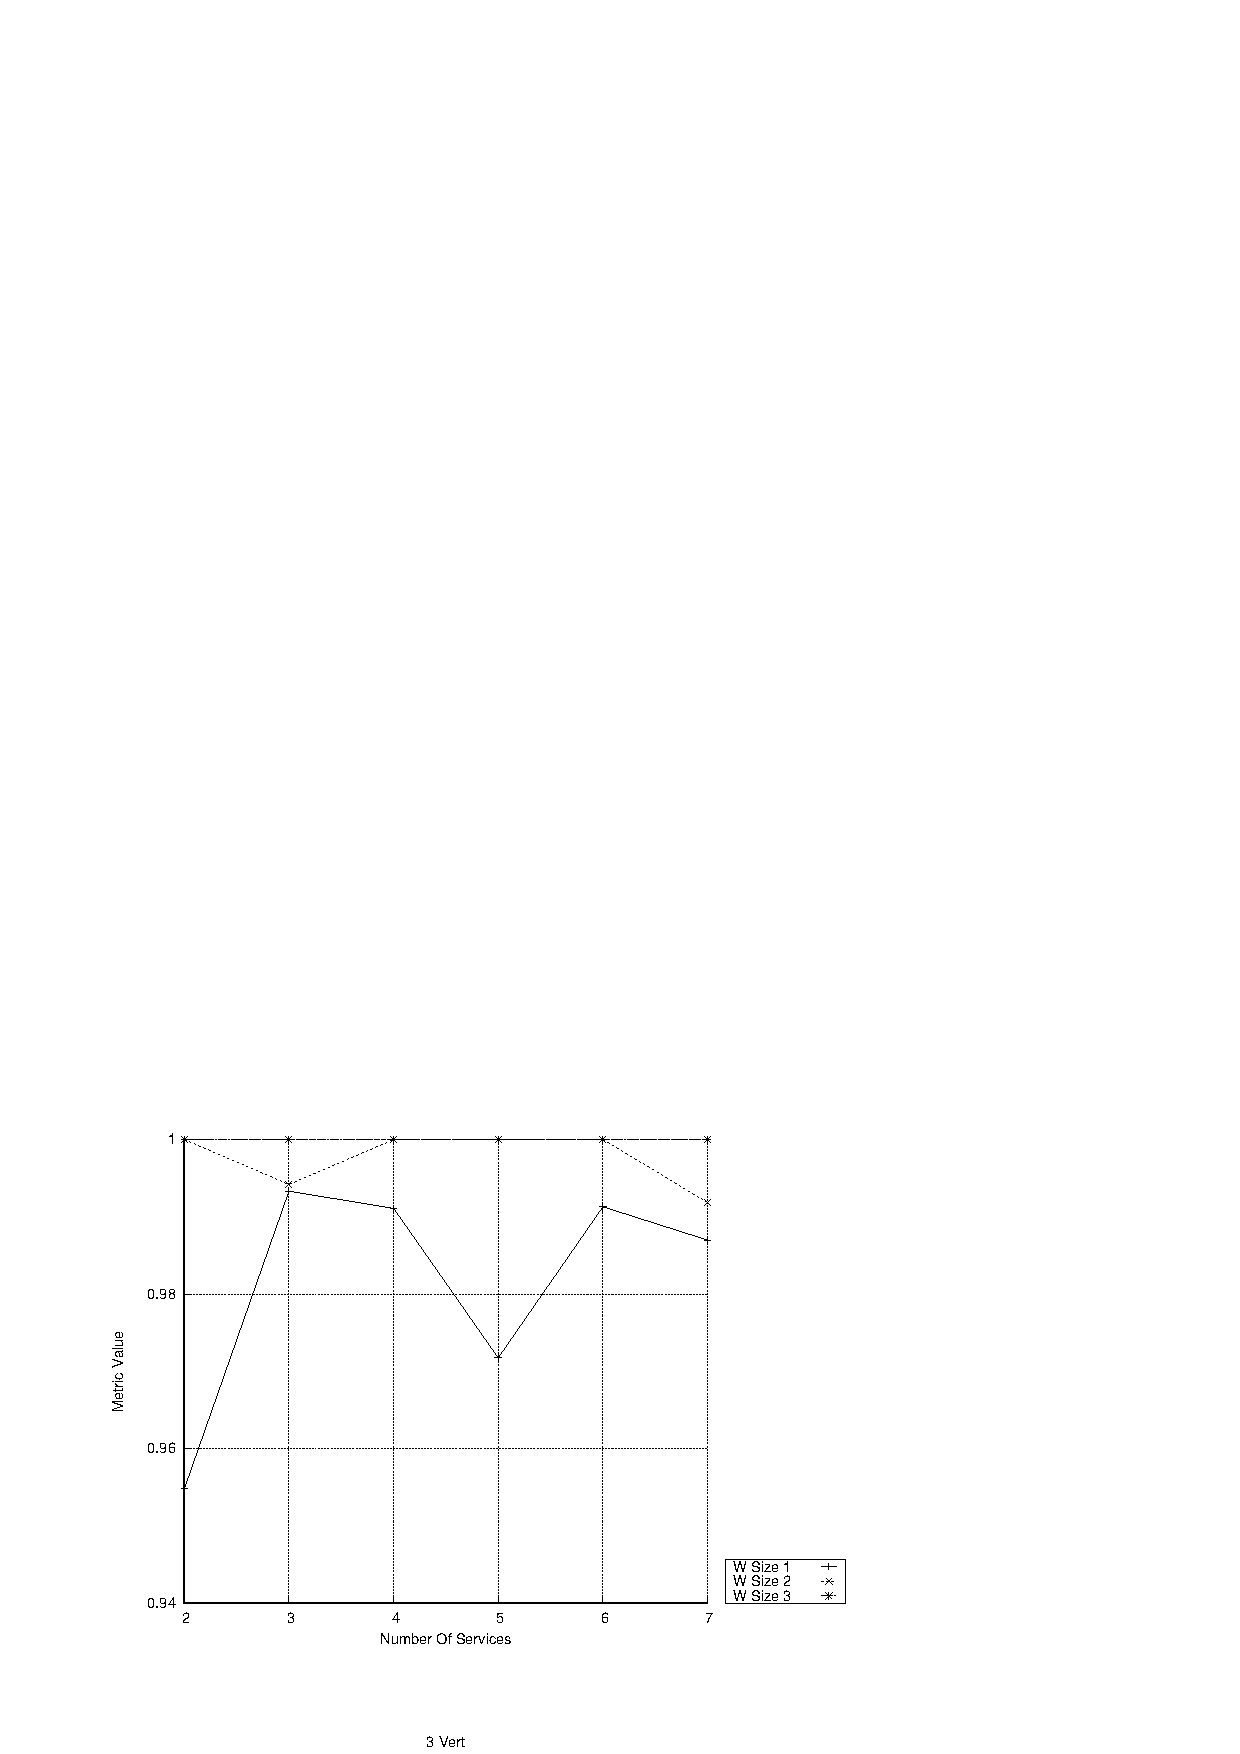
\includegraphics[width=\textwidth]{Images/graphs/window_quality_performance_diff_qual_n7_s7_20_100_n3}
        \caption{\wide 3 vertices}
        \label{fig:quality_window_wide_qualitative_n3}
      \end{subfigure}
      \hfill
      \begin{subfigure}{0.49\textwidth}
        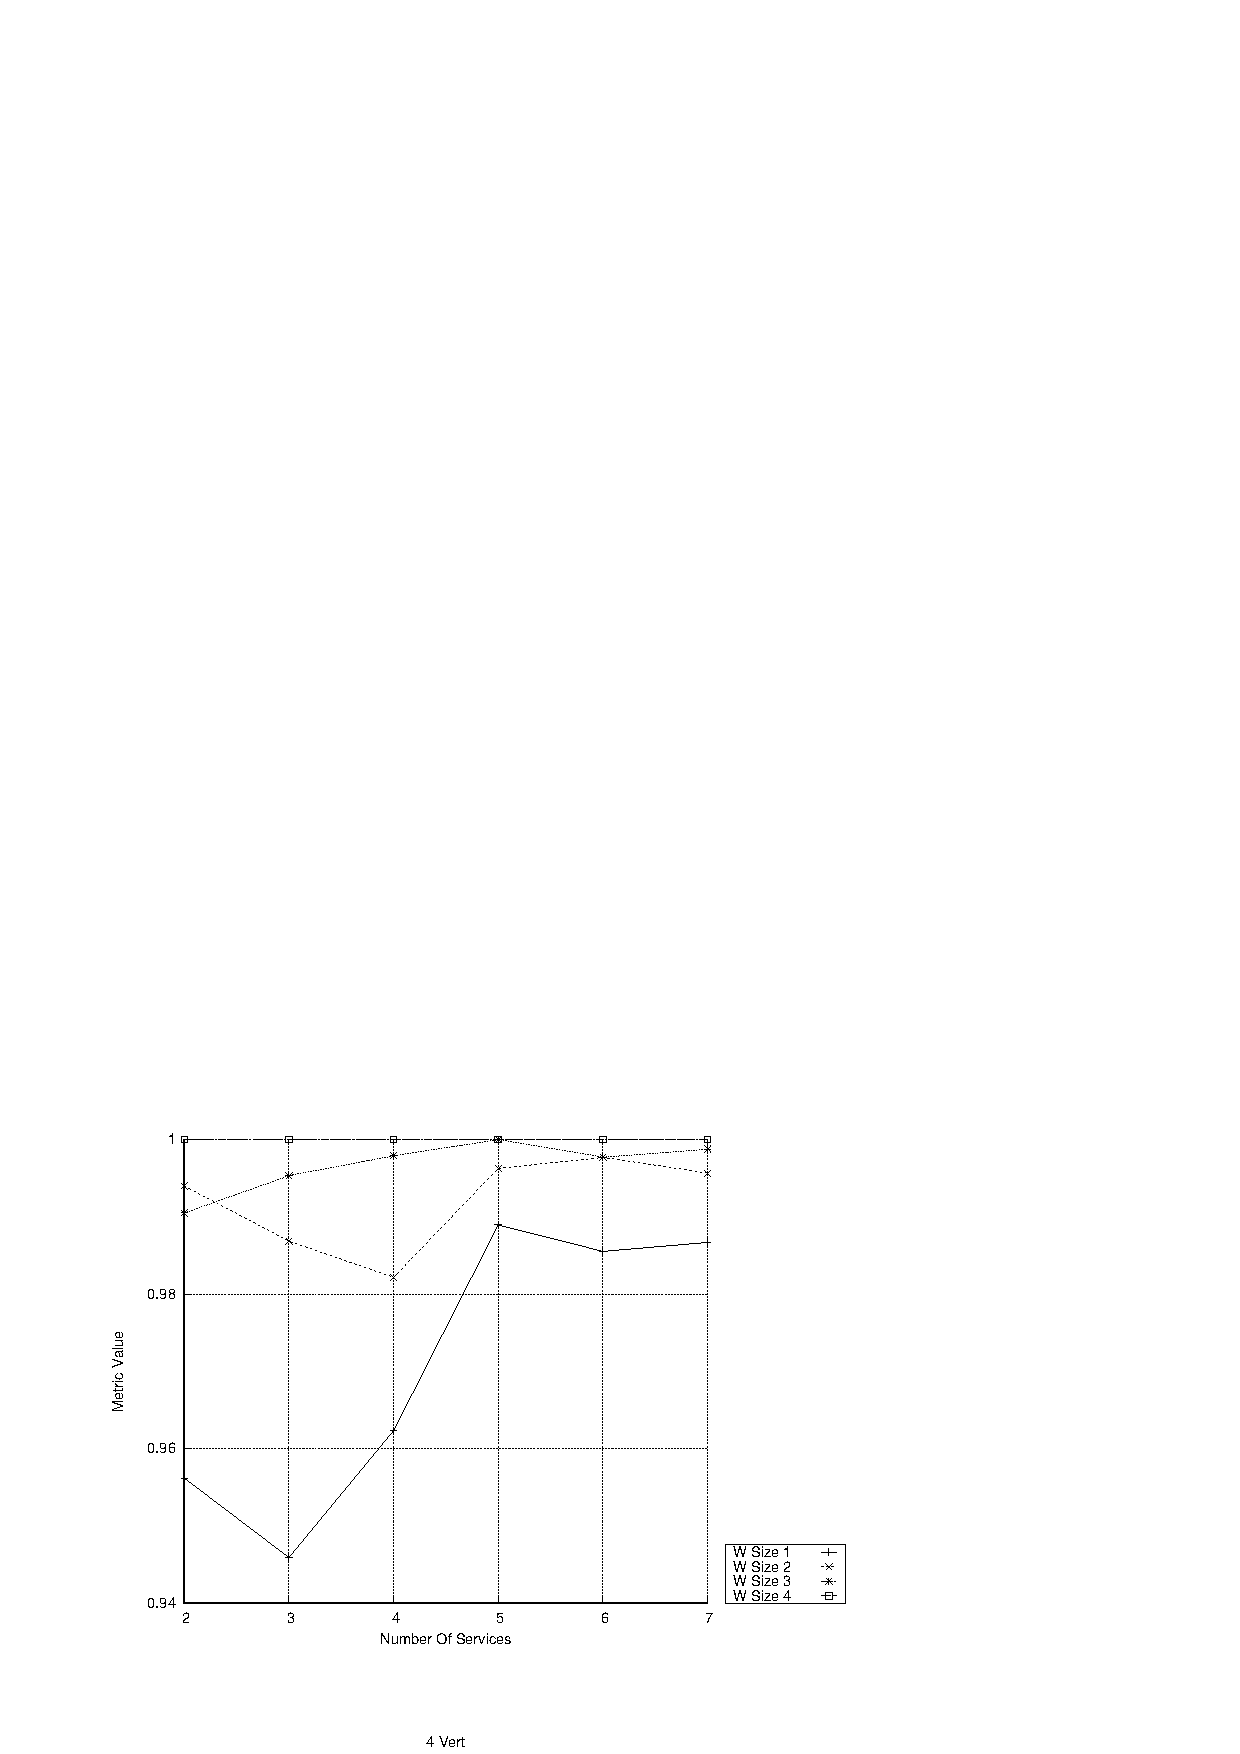
\includegraphics[width=\textwidth]{Images/graphs/window_quality_performance_diff_qual_n7_s7_20_100_n4}
        \caption{\wide 4 vertices}
        \label{fig:quality_window_wide_qualitative_n4}
      \end{subfigure}
      \hfill
      \begin{subfigure}{0.49\textwidth}
        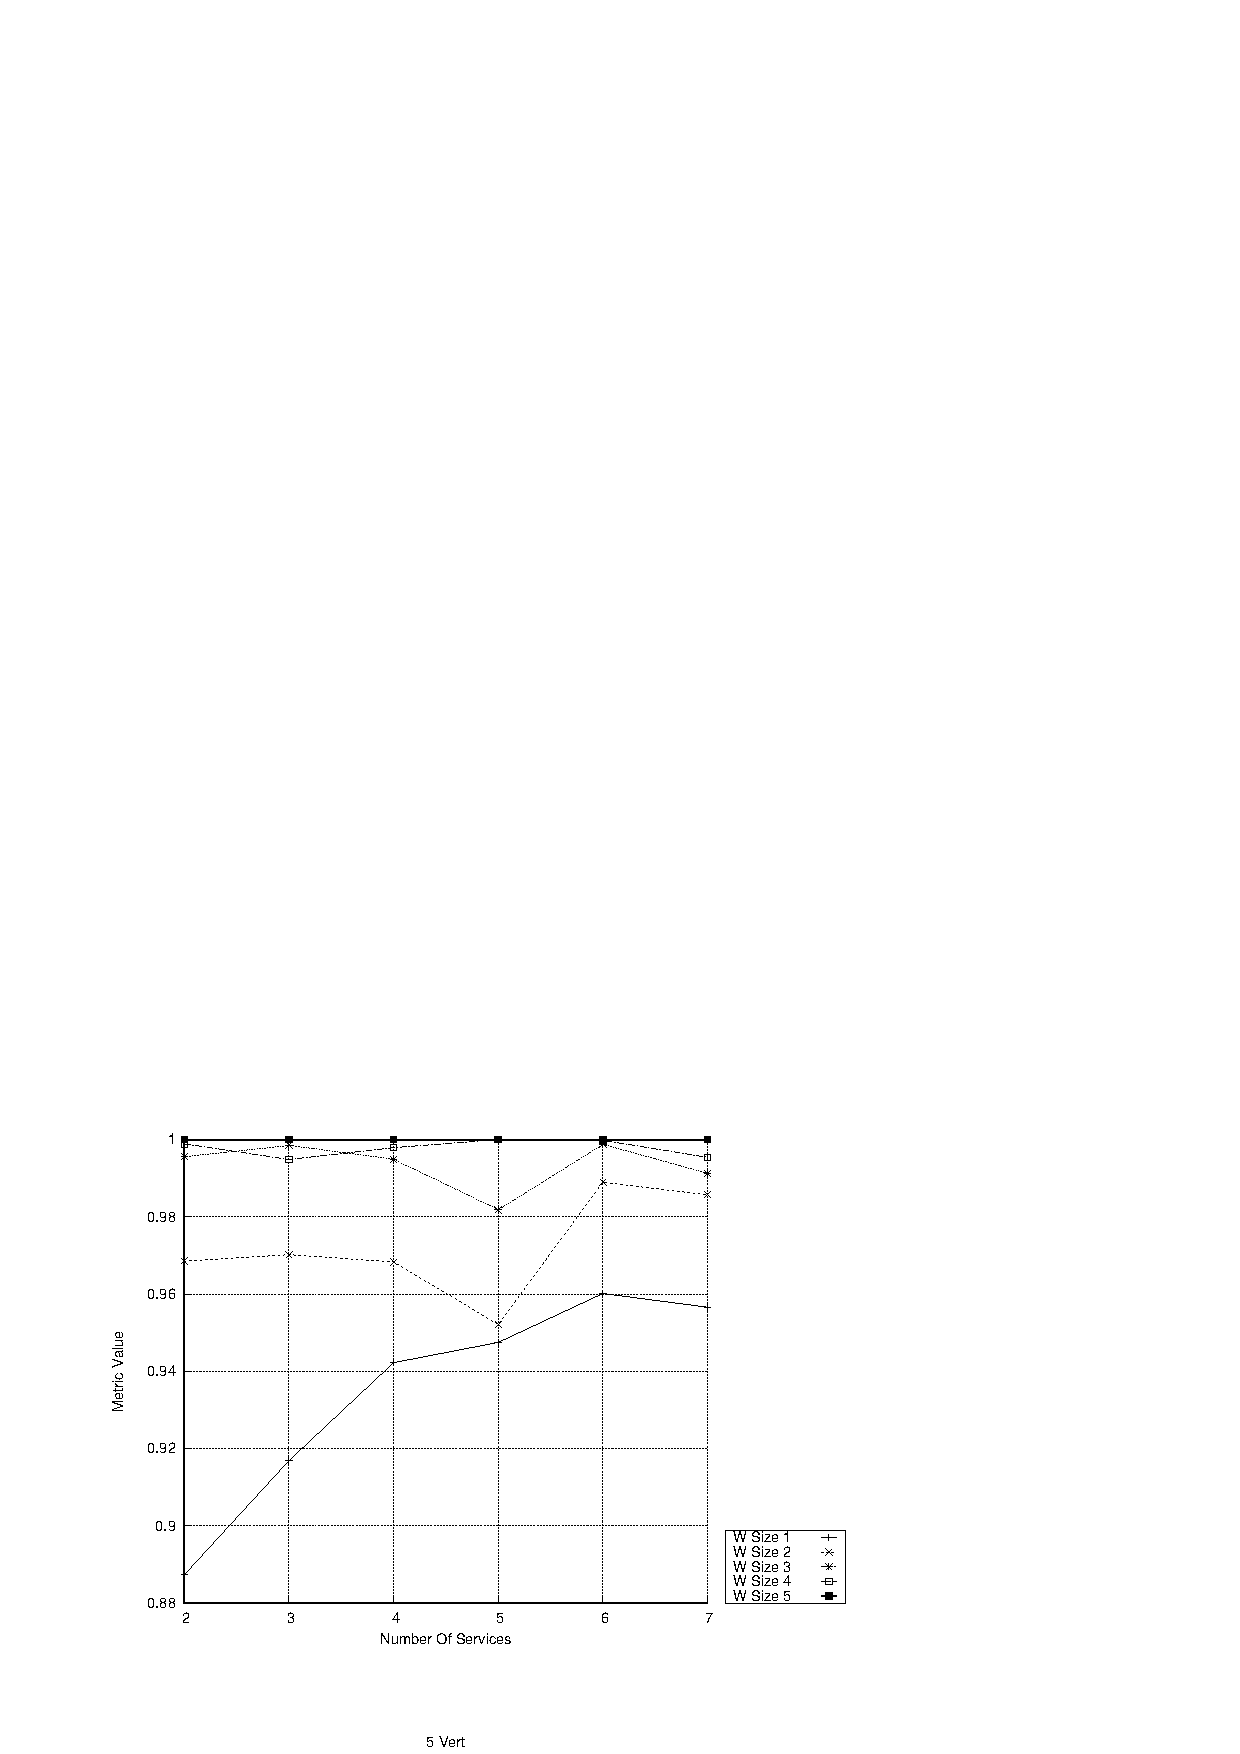
\includegraphics[width=\textwidth]{Images/graphs/window_quality_performance_diff_qual_n7_s7_20_100_n5}
        \caption{\wide 5 vertices}
        \label{fig:quality_window_wide_qualitative_n5}
      \end{subfigure}
      \hfill
      \begin{subfigure}{0.49\textwidth}
        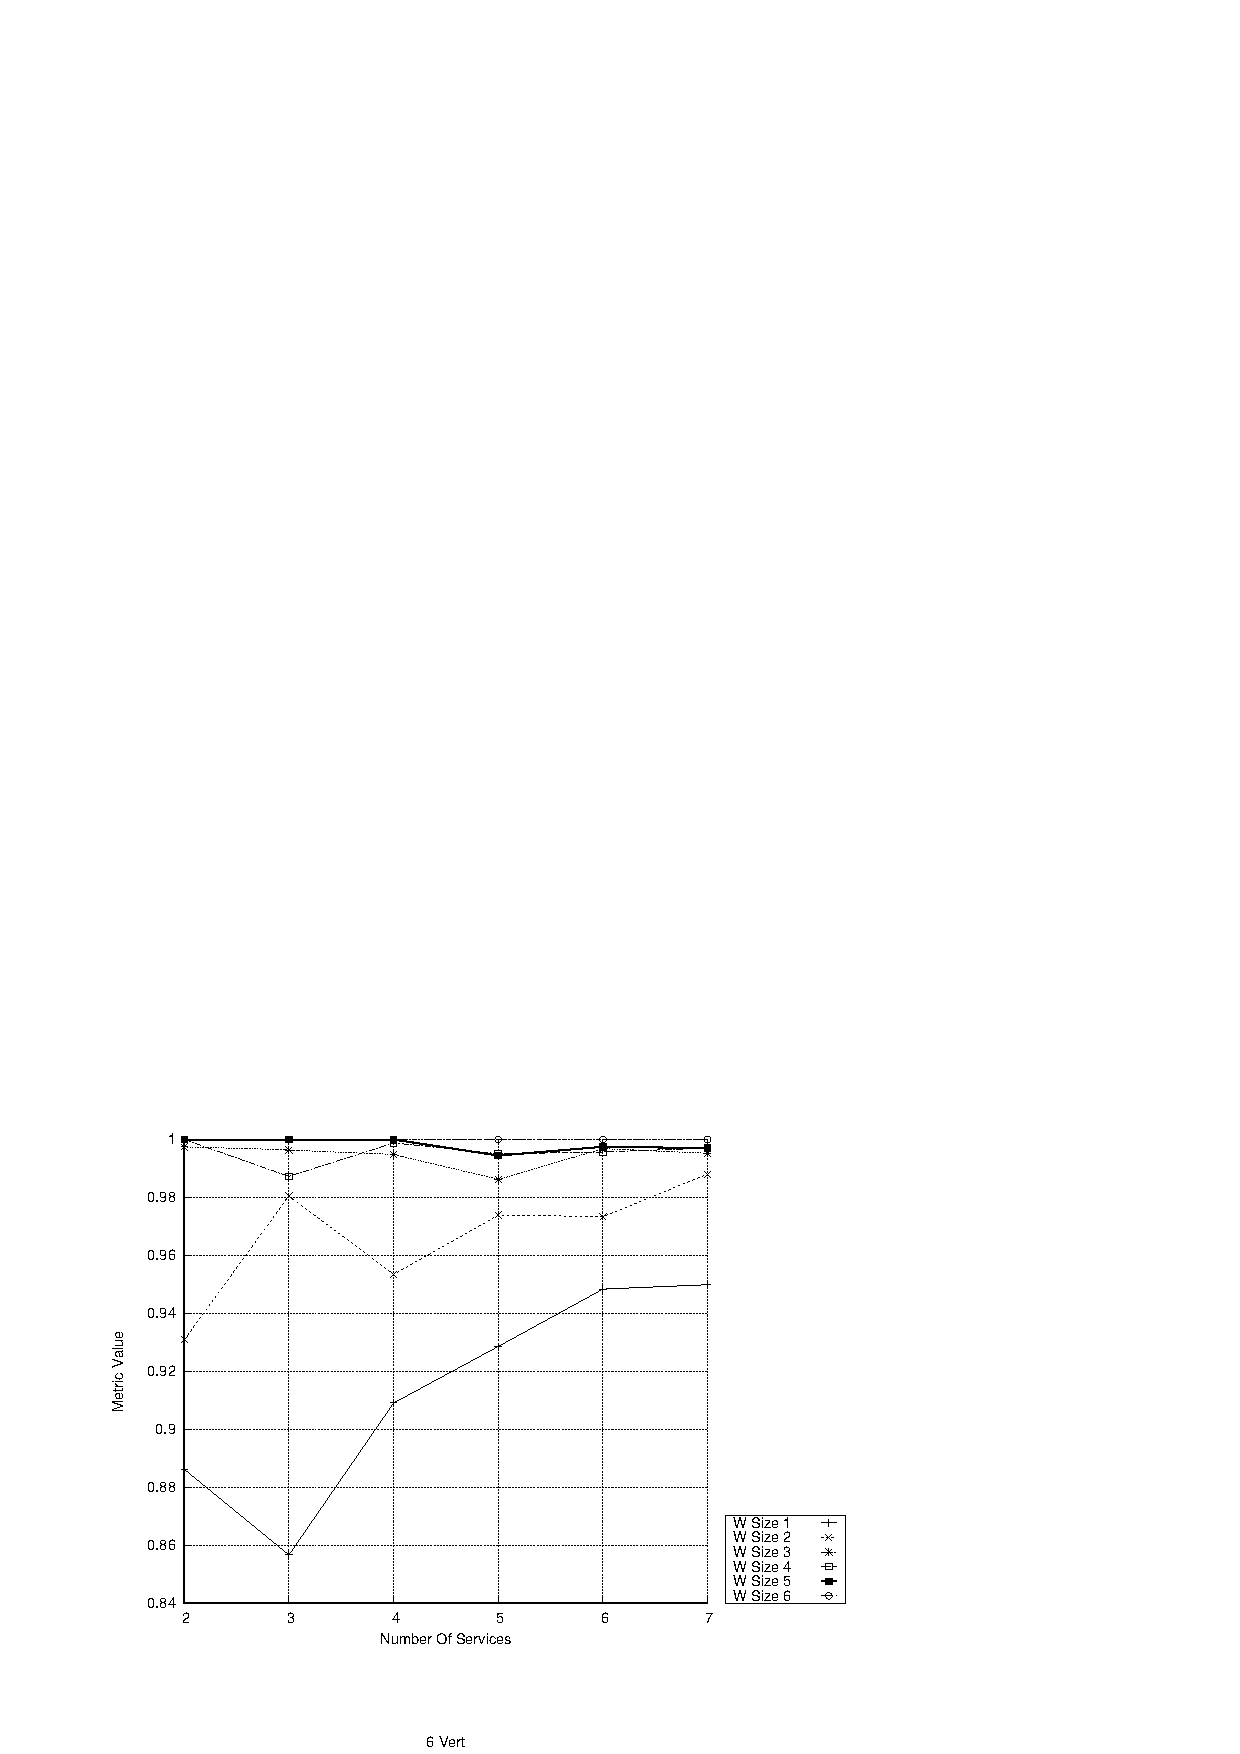
\includegraphics[width=\textwidth]{Images/graphs/window_quality_performance_diff_qual_n7_s7_20_100_n6}
        \caption{\wide 6 vertices}
        \label{fig:quality_window_wide_qualitative_n6}
      \end{subfigure}
      \hfill
      \begin{subfigure}{0.49\textwidth}
        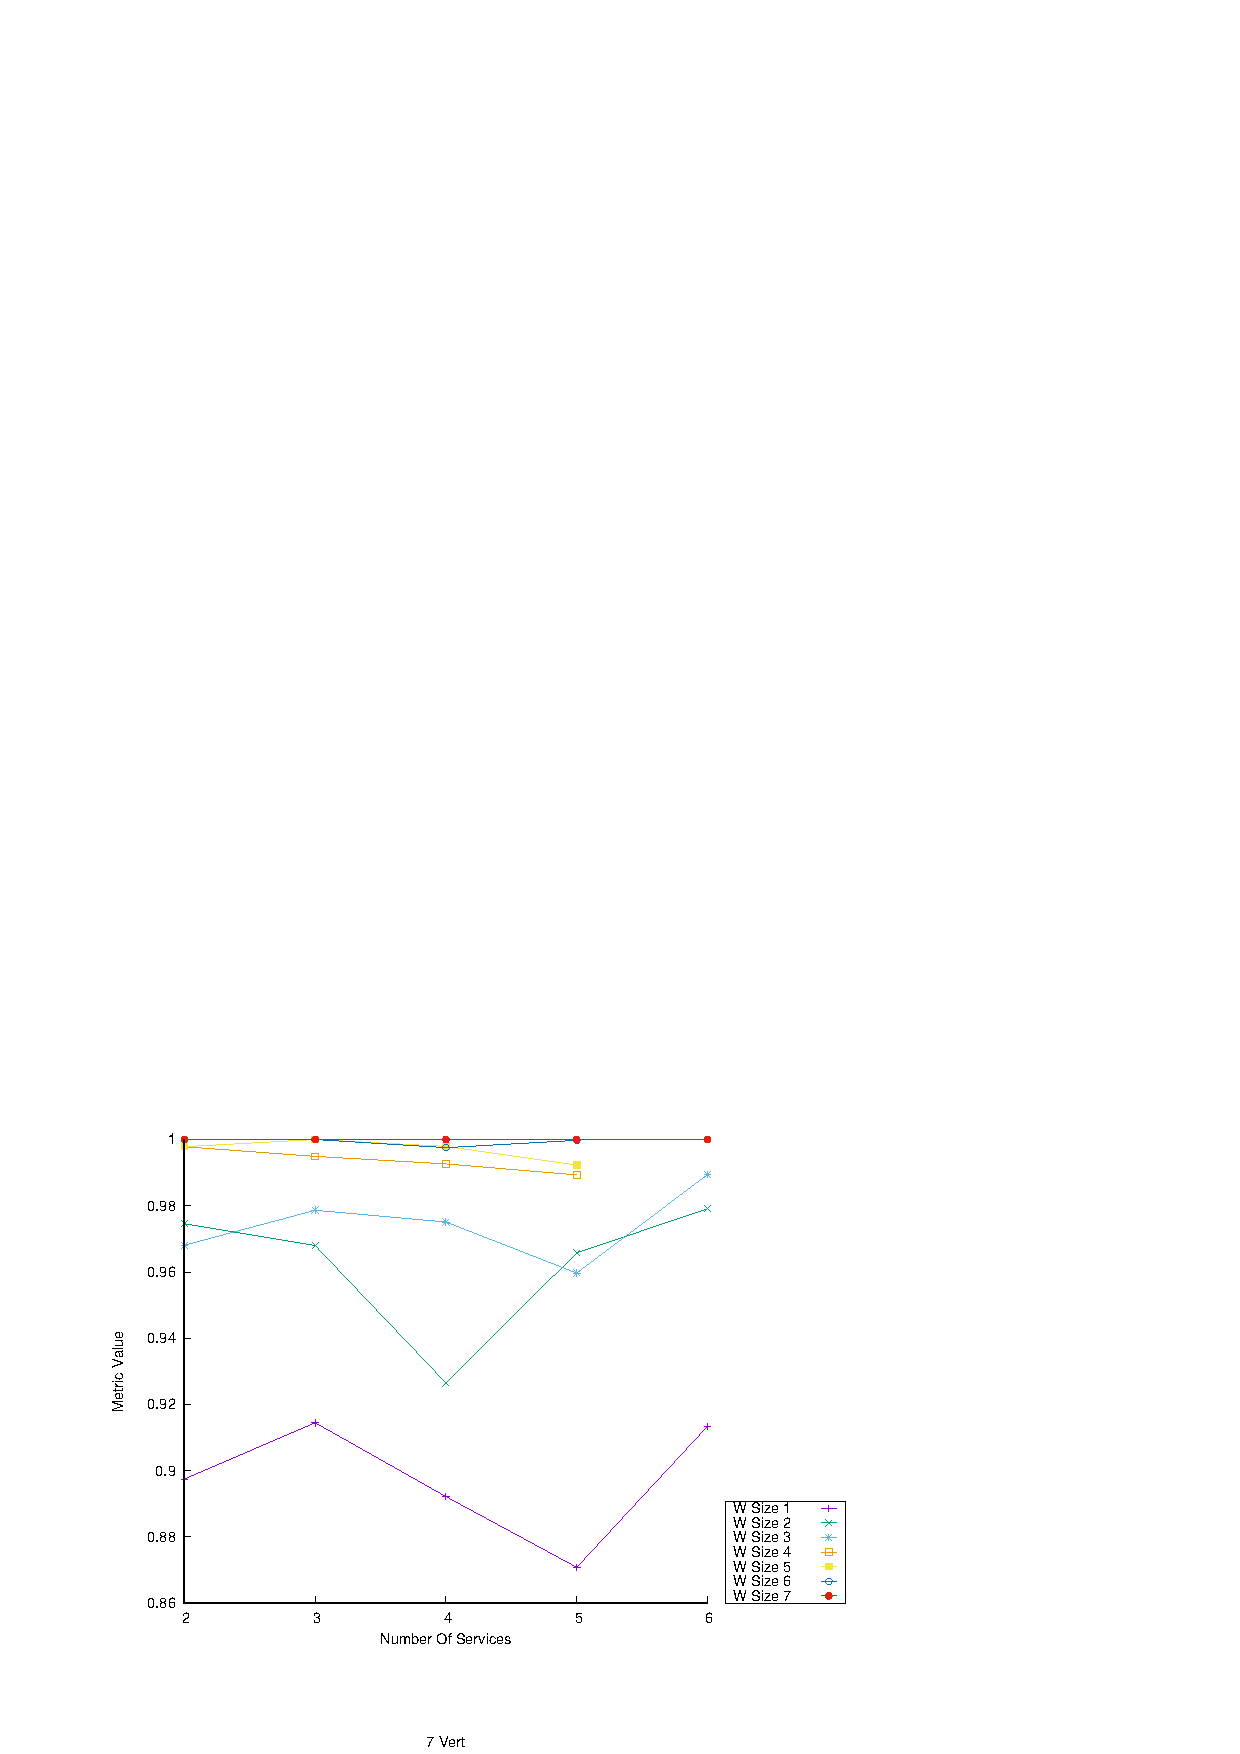
\includegraphics[width=\textwidth]{Images/graphs/window_quality_performance_diff_qual_n7_s7_20_100_n7}
        \caption{\wide 7 vertices}
        \label{fig:quality_window_wide_qualitative_n7}
      \end{subfigure}


      \caption{Evaluation of Quality Using the \emph{Qualitative} Metric in a \wide (\cref{fig:quality_window_wide_qualitative_n3,fig:quality_window_wide_qualitative_n4,fig:quality_window_wide_qualitative_n5,fig:quality_window_wide_qualitative_n6,fig:quality_window_wide_qualitative_n7}) Profile Configuration.}  \label{fig:quality_window_qualitative_wide}
    \end{figure}

    \begin{figure}[H]
      \centering
      \begin{subfigure}{0.49\textwidth}
        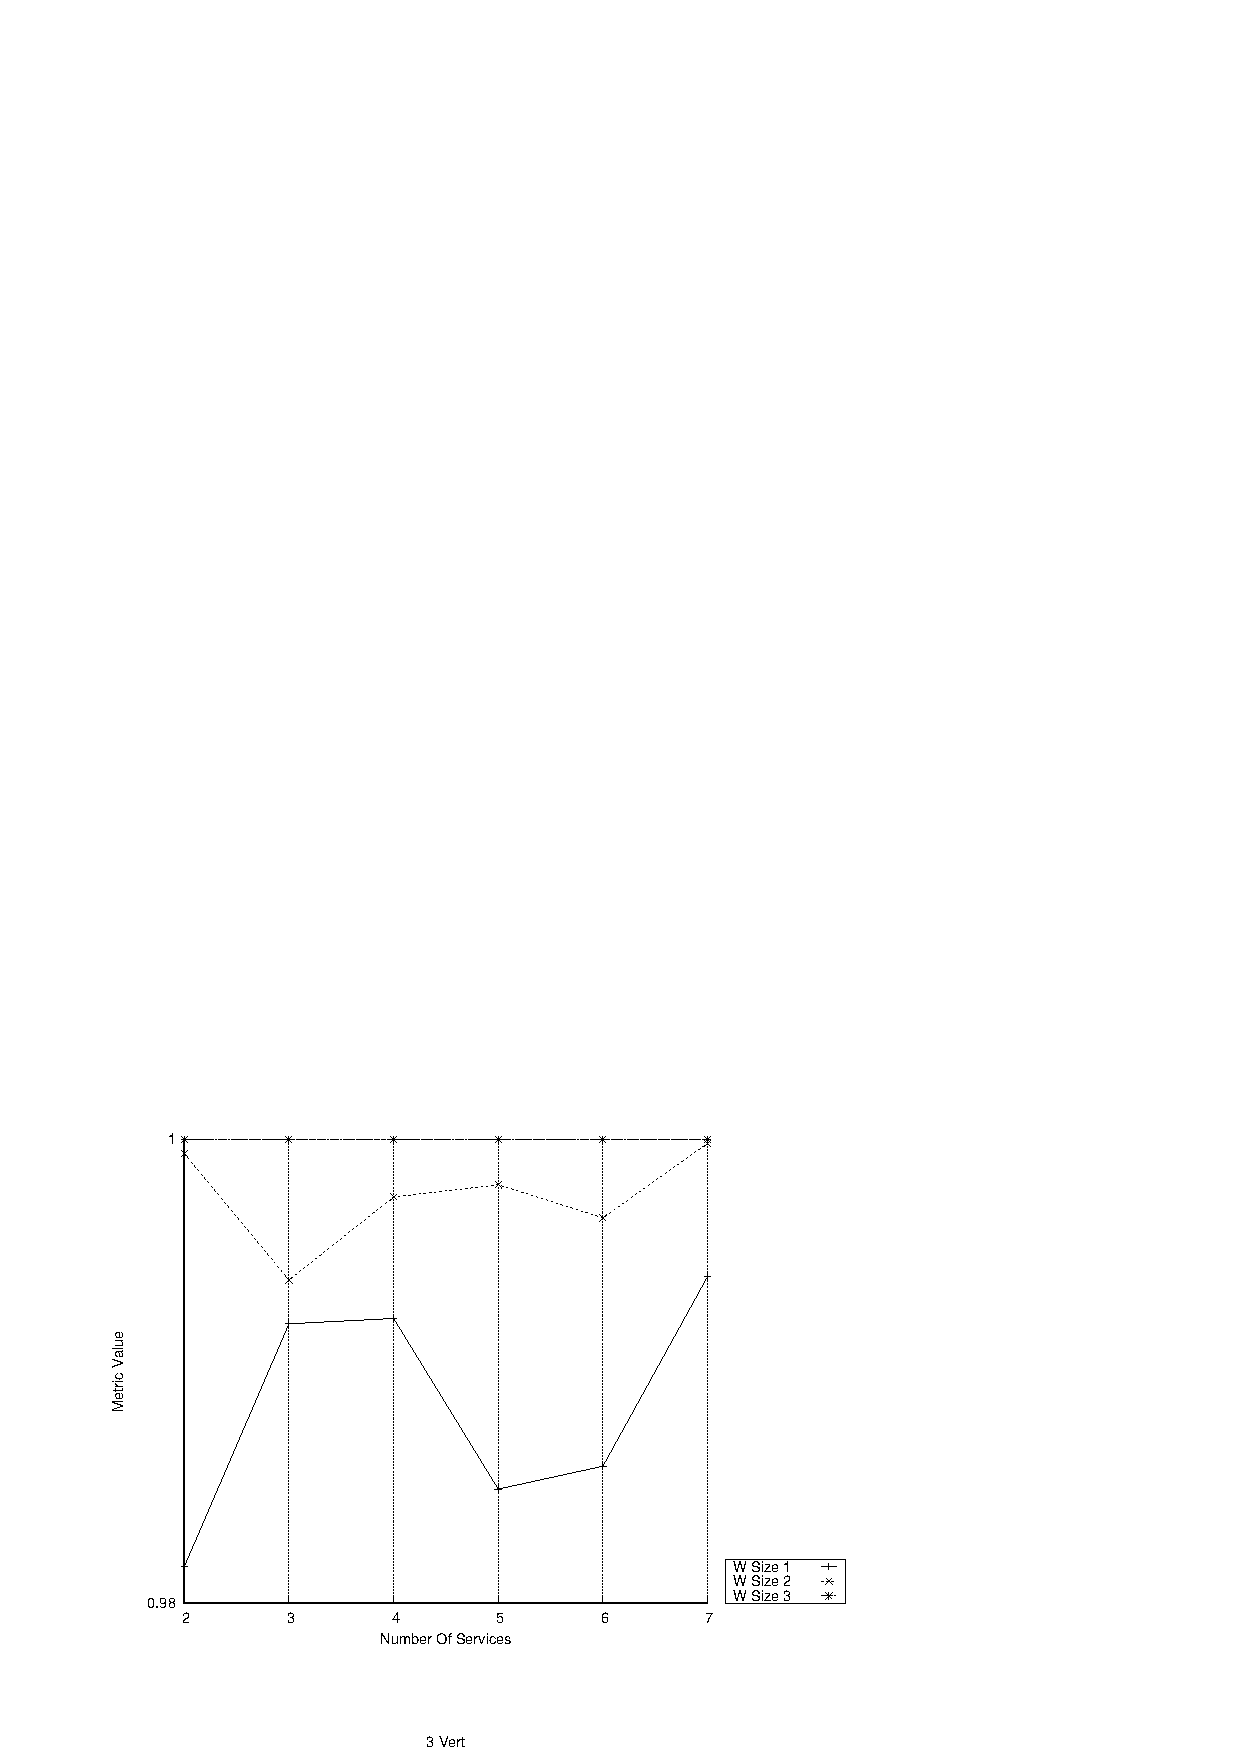
\includegraphics[width=\textwidth]{Images/graphs/window_quality_performance_diff_qual_n7_s7_50_80_n3}
        \caption{\average 3 vertices}
        \label{fig:quality_window_average_qualitative_n3}
      \end{subfigure}
      \hfill
      \begin{subfigure}{0.49\textwidth}
        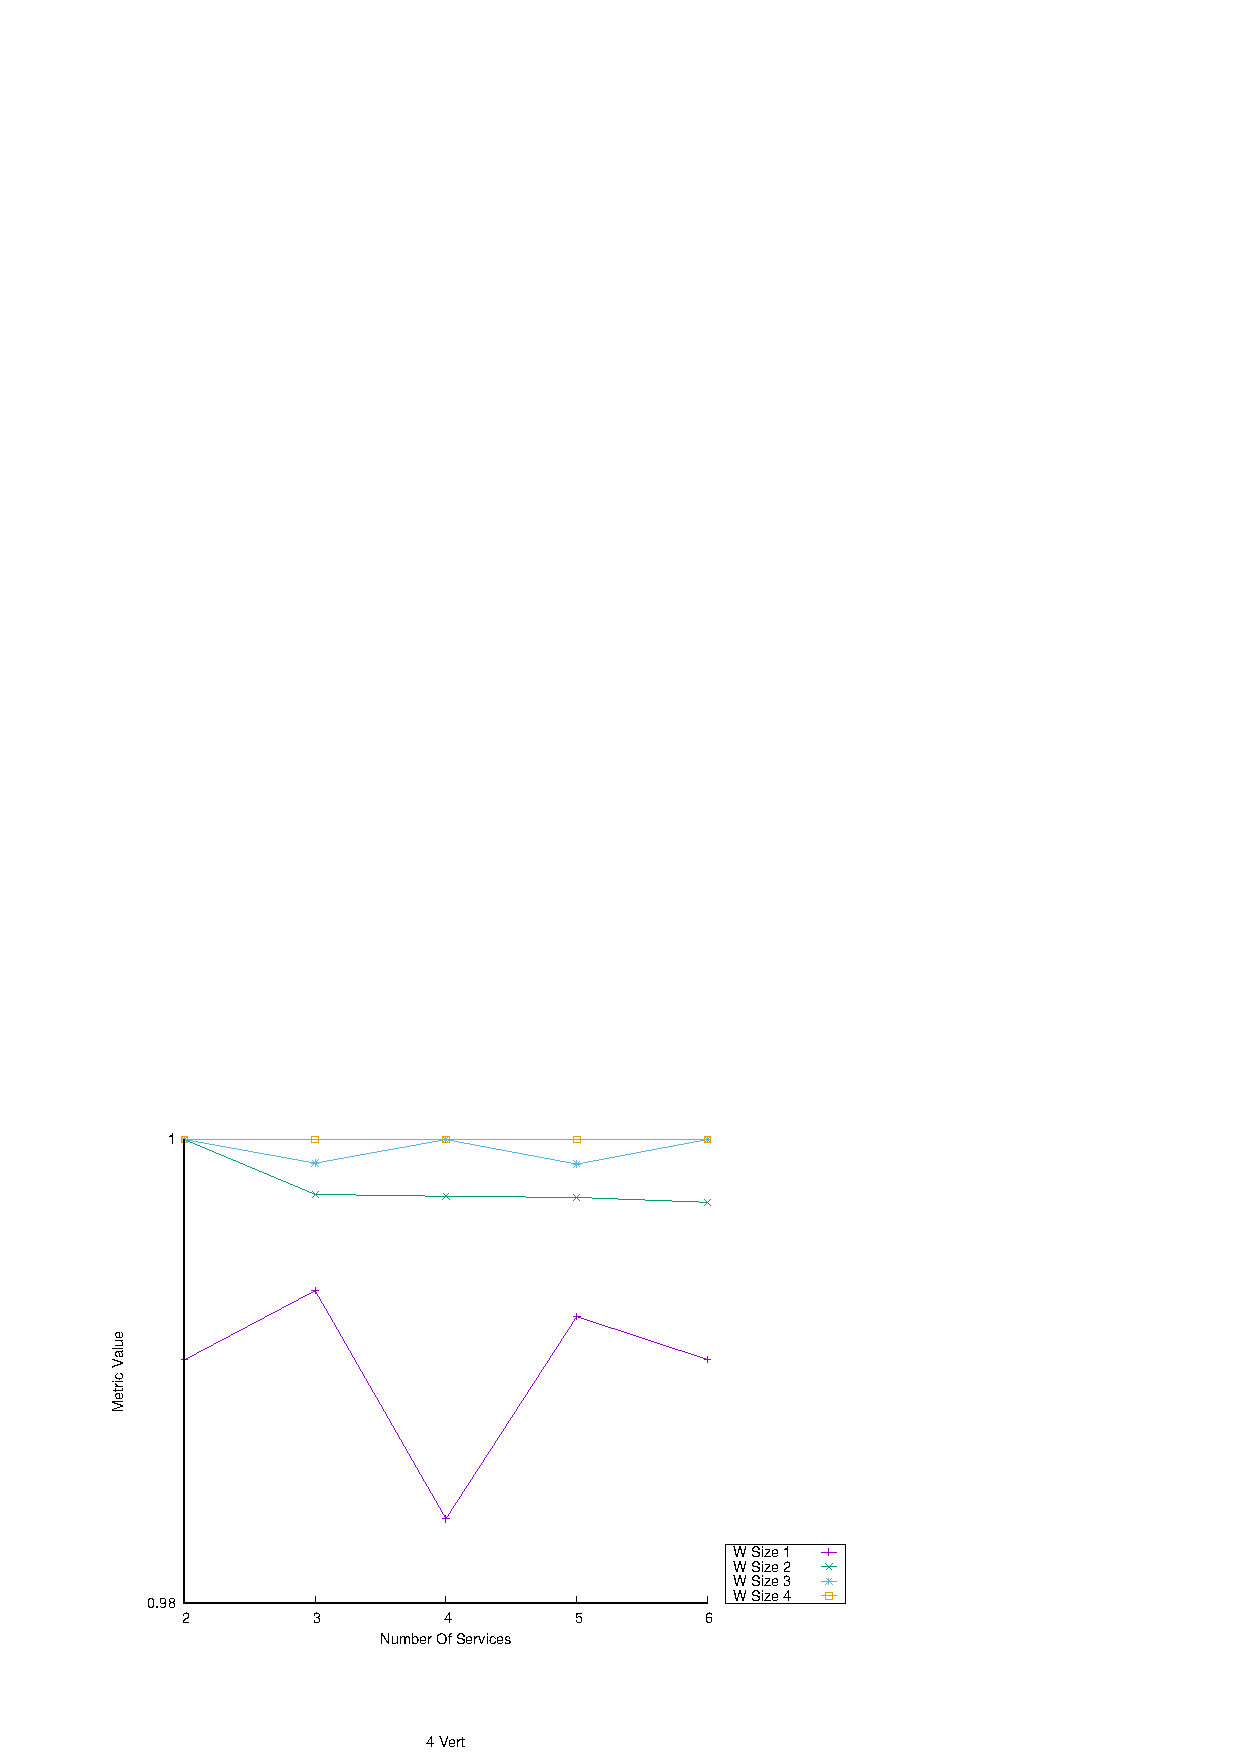
\includegraphics[width=\textwidth]{Images/graphs/window_quality_performance_diff_qual_n7_s7_50_80_n4}
        \caption{\average 4 vertices}
        \label{fig:quality_window_average_qualitative_n4}
      \end{subfigure}
      \hfill
      \begin{subfigure}{0.49\textwidth}
        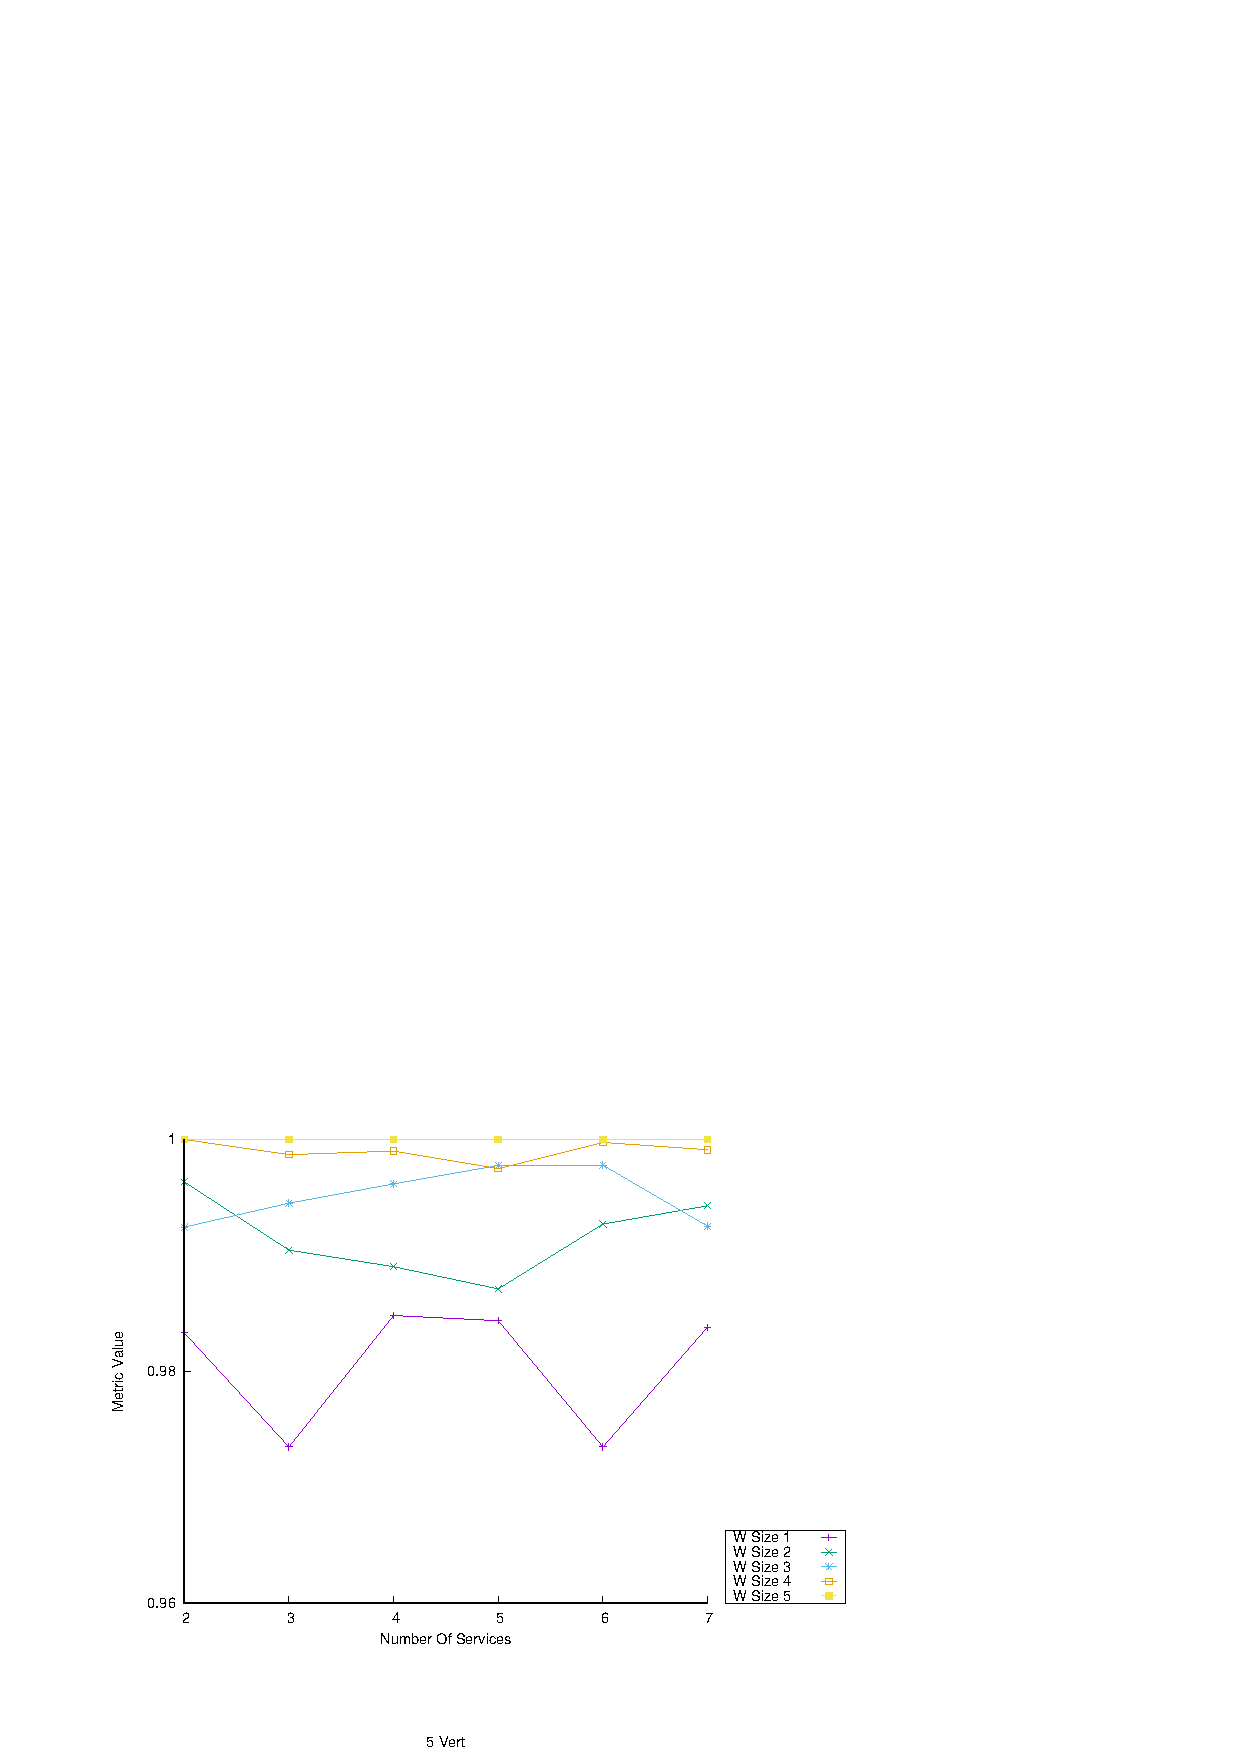
\includegraphics[width=\textwidth]{Images/graphs/window_quality_performance_diff_qual_n7_s7_50_80_n5}
        \caption{\average 5 vertices}
        \label{fig:quality_window_average_qualitative_n5}
      \end{subfigure}
      \hfill
      \begin{subfigure}{0.49\textwidth}
        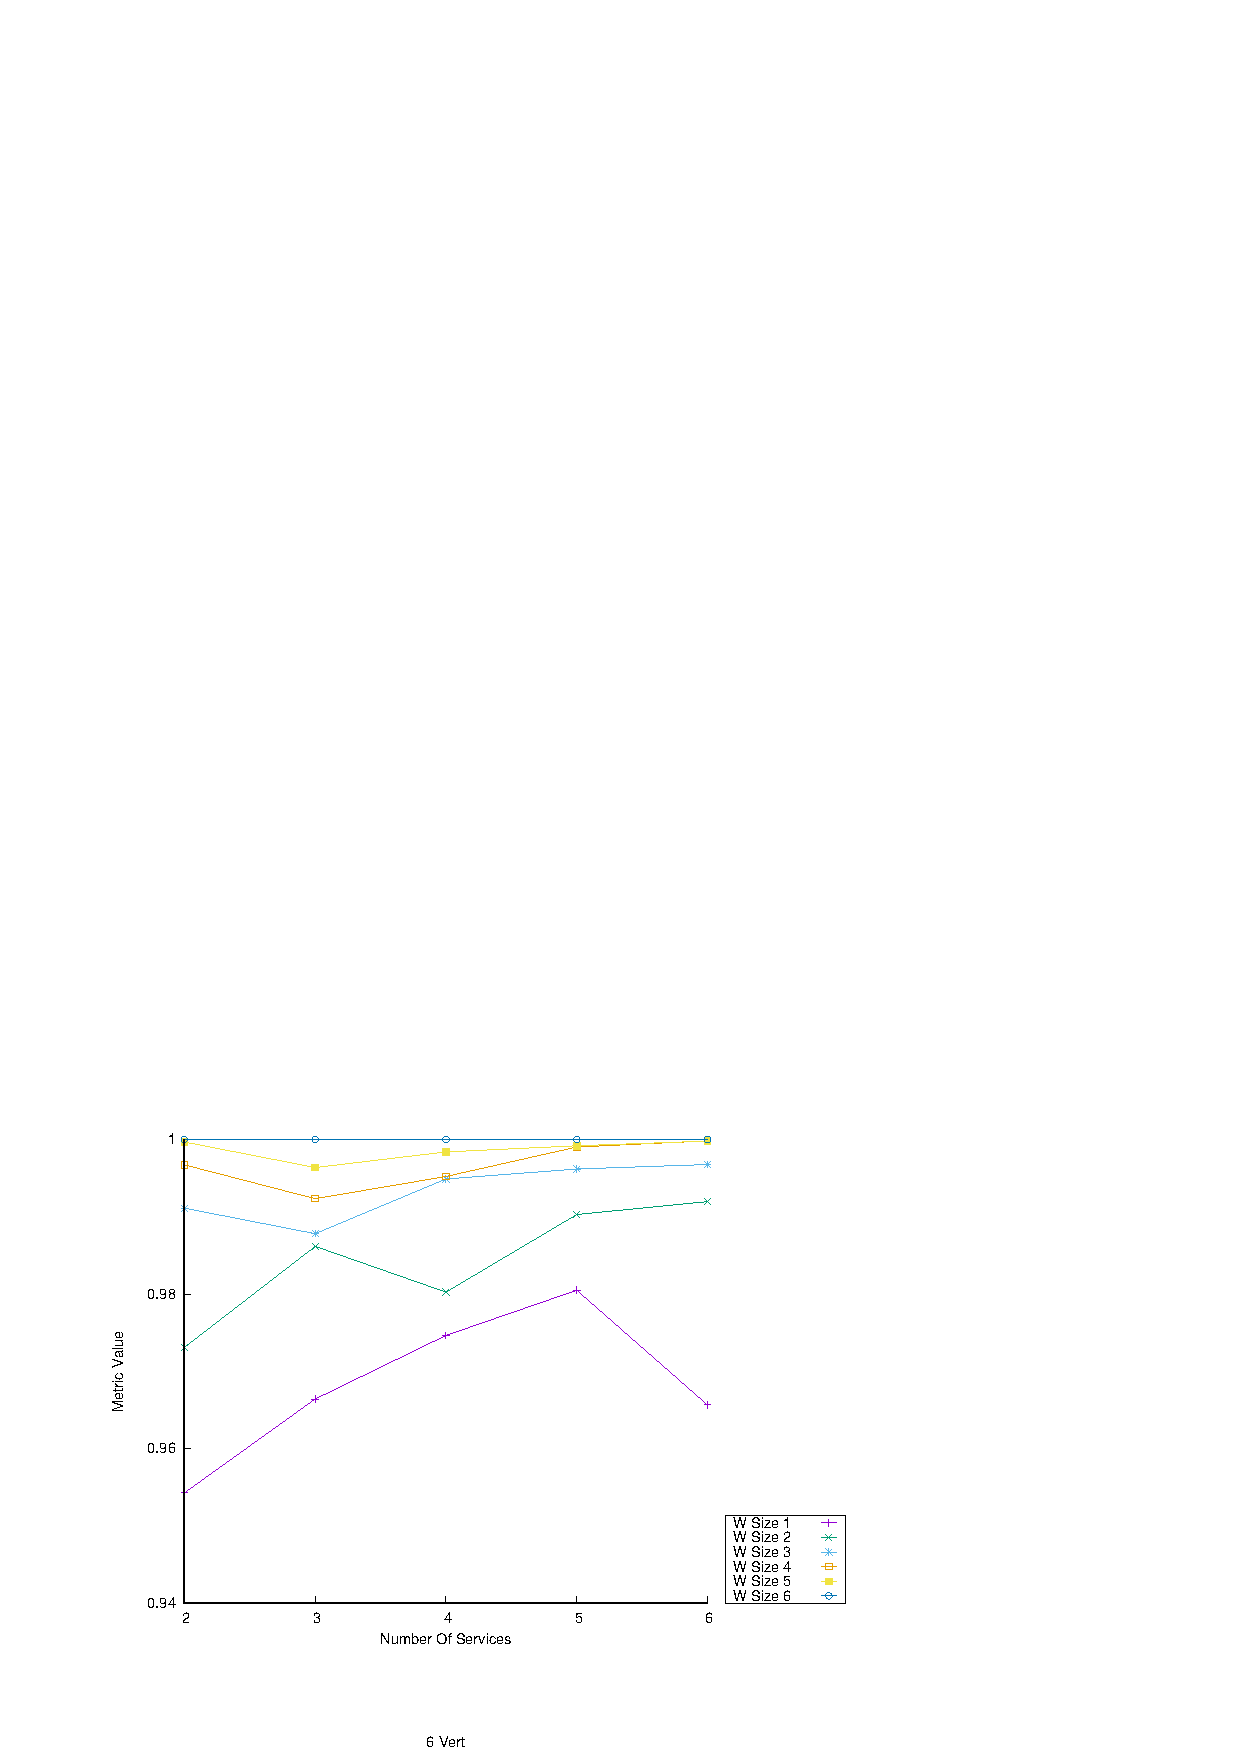
\includegraphics[width=\textwidth]{Images/graphs/window_quality_performance_diff_qual_n7_s7_50_80_n6}
        \caption{\average 6 vertices}
        \label{fig:quality_window_average_qualitative_n6}
      \end{subfigure}
      \hfill
      \begin{subfigure}{0.49\textwidth}
        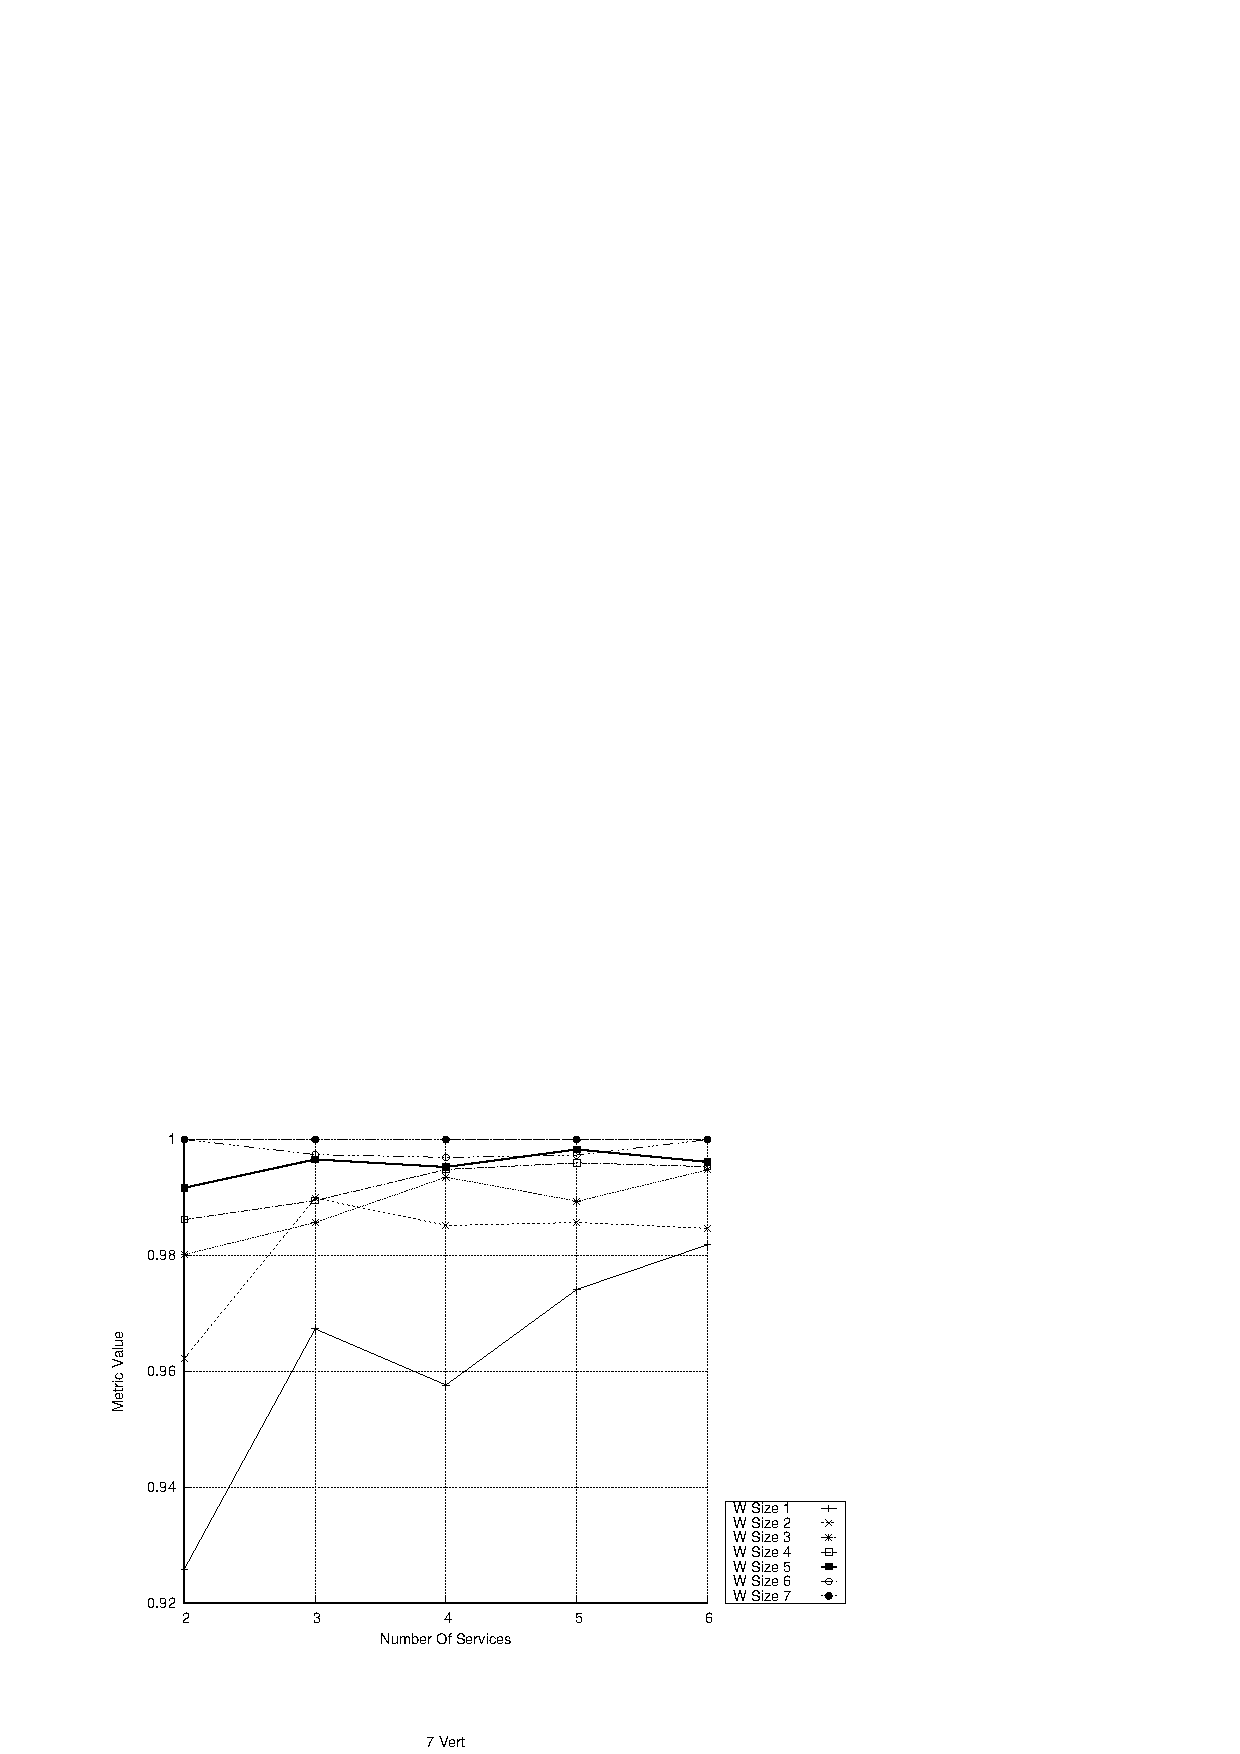
\includegraphics[width=\textwidth]{Images/graphs/window_quality_performance_diff_qual_n7_s7_50_80_n7}
        \caption{\average 7 vertices}
        \label{fig:quality_window_average_qualitative_n7}
      \end{subfigure}

      \caption{Evaluation of Quality Using the \emph{Qualitative} Metric in an \average (\cref{fig:quality_window_average_qualitative_n3,fig:quality_window_average_qualitative_n4,fig:quality_window_average_qualitative_n5,fig:quality_window_average_qualitative_n6,fig:quality_window_average_qualitative_n7}) Profile Configuration.}  \label{fig:quality_window_qualitative_average}

    \end{figure}

    When considering configuration \average, the baseline (\windowsize=1) provides results similar to configuration \wide. On average, quality varies from 0.920 to 0.969, limiting oscillations; for instance, the quality varies between 0.951 and 0.989 for $l$=3, 0.942 and 0.988 for $l$=4, 0.919 and 0.975 for $l$=5, 0.912 and 0.972 for $l$=6, 0.878 and 0.925 for $l$=7. The \average configuration provides even tighter quality oscillations than the \wide configuration. Notably, the poorest quality outcomes are observed with the baseline. Conversely, these oscillations become negligible when the window size exceeds 1 in configurations with three and four vertices, and when it exceeds 2 in configurations involving five, six, and seven vertices.  For instance, when \windowsize=3, the quality varies between  0.993 and 1 for $l$=4, 0.981 and 0.998 for $l$=5, 0.982 and 997 for $l$=6, 0.960 and 0.991 for $l$=7.


\subsection{Discussion}
The experimental results we obtained yield several valuable insights that merit further discussion. Three key observations emerged as follows.

\vspace{0.5em}

\noindent\textbf{Trade-off Between Execution Time and Quality.} As expected, the execution time improvement provided by our heuristic introduces a loss of quality with respect to the exhaustive approach. This loss causes an increase in the quality variance, especially when the window size (\windowsize) is small compared to the vertex count. A fine-grained tuning of heuristics is needed to balance computational efficiency and data quality.

\vspace{0.5em}

\noindent\textbf{Impact of Parameters on Quality.}
{\color{OurColor2}

  Our experiments demonstrate that parameters in Table~3 can significantly influence the quality of the pipeline, with the pipeline template length and the window size emerging as key factors for both quality and performance.

  Specifically, larger window sizes generally improve quality; however, there exists a balance point where the trade-off between computational cost and quality gain becomes suboptimal. Beyond this threshold, additional computational resources do not proportionately enhance data quality, as modeled by our metrics.
  We also note that lower window sizes exhibit higher instability, particularly under the \wide configuration, where data quality varies significantly across different setups. This variation diminishes when larger window sizes, approximately half the length of the pipeline (e.g., \windowsize$=$$l$/2), are used, leading to more stable and consistent results.

  We also note that the number of candidate services and service nodes increases the computation cost (performance) with a minor impact on quality (on average).

  In conclusion, our results demonstrate a significant reduction in computational overhead, while
  maintaining high data quality. Further analysis is needed to explore the impact of additional parameters, first of all in terms of diverse datasets modeling additional real-world domains, to understand their broader impact on quality. Investigating alternative quality metrics could also provide new insights and opportunities for improvement. Future experiments, as outlined in Section 9, will aim to address these aspects to provide a step further in the evaluation of the soundness and applicability of our framework on a larger scale.
}
\vspace{0.5em}

\noindent\textbf{Sliding Window Approach versus Global Awareness.} The intrinsic nature of our sliding window heuristic can sometimes lead to a local optimum, as the window size limits the candidate services for each pipeline stage to a restricted subset, which may prevent reaching the global optimum. This aspect is maximized when using the baseline representing the state of the art, where the sliding window heuristic is configured with a window size of \windowsize=1. Additionally, as dependencies between services increase, the likelihood of finding a sub-optimal solution rises. Our experiments show that \emph{i)} increasing the window size helps mitigate this issue and \emph{ii)} a broader decision-making scope becomes essential as service dependencies grow more complex.


\section{Related Work}\label{sec:related}


In this related work section, we address two fundamental challenges in the field of data protection for service-based pipelines. 
In Section  \ref{sec:dataquality}, we address the issue of the lack of consensus on the definition of data quality and, consequently, on data quality metrics when applying data protection transformations. In Section \ref{sec:datagov}, we examine existing data governance solutions that tackle the problem of data protection when sharing data among different services.

%%%%%%%%%%%%%%%%%%%%
\subsection{Data quality and data protection}\label{sec:dataquality}
%%%%%%%%%%%%%%%%%%%%

%Data quality is a widely studied research topic across various communities and perspectives, such as the database community or when evaluating privacy preserving data mining techniques. In the context of big data, data quality primarily refers to the extent to which big data meets the requirements and expectations of its intended use, encompassing various dimensions and characteristics to ensure the data is reliable, accurate, and valuable for analysis and decision-making. Specifically, accuracy denotes the correctness of the data, ensuring it accurately represents the real-world entities and events it models.
Data quality is a widely studied research topic studied across various communities and perspectives. In the context of (big) data pipelines, data quality primarily refers to the extent to which (big) data meets the requirements and expectations of its intended use, encompassing various dimensions and characteristics to ensure the data are reliable, accurate, and valuable for analysis and decision-making. Specifically, accuracy denotes the correctness of the data, ensuring it accurately represents the real-world entities and events it models.

With the increasing need to protect sensitive data, the notion of data quality has expanded to include a broader concept of accuracy, particularly in terms of the proximity of a sanitized value to the original value.
This shift has emphasized the need of metrics to assess the quality of data resulting from anonymization processes. 
Differential privacy \cite{dwork2008differential}, k-anonymity \cite{k-anon}, and l-diversity \cite{l-diversity} are three distinct techniques used to provide data anonymization, with different protection levels and results on data quality. For example, differential privacy is highly effective in maintaining confidentiality, but the noise added can reduce data precision, impacting analytical accuracy, whereas k-anonymity and l-diversity generally maintain higher data quality than differential privacy, but they might still be unable to protect against sophisticated attacks.

Various data quality metrics have been proposed in existing literature, including generalized information loss (\textit{GenILoss}), discernability metric, minimal distortions, and average equivalence class size ($C_{AVG}$), which may either have broad applicability or be tailored to specific data scenarios \cite{Majeed2021AnonymizationTF,bookMetrics,reviewMetrics}. However, there is currently no metric that is widely accepted by the research community. The main challenge with data quality is its relative nature: its evaluation typically depends on the context in which the data is used and often involves both objective and subjective parameters \cite{dataAccuracy,dataQuality}.
%
A common consideration across all contexts is that accuracy is closely related to the information loss resulting from the anonymization strategy: the lower the information loss, the higher the data quality. In our scenario, we have opted for two generic metrics rooted in data loss assessment (i.e., data completeness) - one quantitative and one qualitative. Nonetheless, our framework and heuristic are designed to be modular and flexible, accommodating the chosen metric.

{\color{OurColor} While existing techniques have provided sound and effective solutions that guarantees data quality and data protection, they often unsuit to scenarios aiming to maximize data quality while ensuring data protection, have limited expressiveness (e.g., the definition of $k$ when $k$-anonymity is used to protect data), are not applicable to pipelines orchestrating services owned by different providers. Our solution fills in the above gaps, by providing a framework for service-based data pipelines that support the selection of data processing services that maximize data quality, while upholding privacy and security requirements. Service selection is driven by high-expressive policies, where data transformations built on data protection techniques (e.g., $k$-anonymity) are applied to data before they are used in the pipeline.} 

%%%%%%%%%%%%%%%%%%
\subsection{Data quality and data protection in service-based pipelines}\label{sec:datagov}
%%%%%%%%%%%%%%%%%%

As organizations increasingly realize the practical benefits and significant value of big data, they also acknowledge the limitations of current big data ecosystems, especially in terms of data governance. In this context, the need for privacy-aware systems enforcing sensitive data protection without compromising data quality throughout the entire data lifecycle arises. Recently, both industry and academia have begun to investigate the issue, recognizing the need of new security requirements \cite{Colombo:JournCybersec:2019} and the importance of addressing the conflict between the need to share and the need to protect information \cite{balancingact,VANDENBROEK2018330,balancingInMedicine,needtobalance,dataProtection}, from a data governance perspective \cite{al2018exploring,aissa2020decide}, and, more in general, to ensure compliance of (big) data pipelines with generic non-functional requirements \cite{ABBJ.ICWS2022,ABHKKS.BD2023}.

The pipeline template proposed in this work addresses these challenges by enabling to express the security policies at the right level of granularity, considering individual services in the pipeline. It can also be easily mapped onto specific platforms, such as Apache-based systems, as we have demonstrated in \cite{medes2021}.
Table \ref{tab:comparative} provides a comparative analysis with relevant existing approaches, highlighting how few industrial solutions compare to our framework according to the following critical features:
\begin{itemize}
    \item \textbf{F1 -- Service-Based Pipeline Support in the Cloud-Edge Continuum:} The ability to effectively operate within distributed environments spanning cloud and edge infrastructure.
    \item \textbf{F2 -- Quality-Aware Service Selection Ensuring Data Protection:} The capacity to optimize service selection processes, maintaining data quality across the pipeline and ensuring robust data protection measures.
    \item \textbf{F3 -- Framework-Agnostic Data Protection:} The degree to which each solution is bound to specific data protection techniques. 
    \item \textbf{F4 -- Policy Expressiveness:} The degree to which each solution supports fine-grained specification of policies or privacy measures.
\end{itemize}

\begin{table}[t!]
    \centering
    \renewcommand{\arraystretch}{1.5}
    \resizebox{\textwidth}{!}{%
    \begin{tabular}{lp{3cm}p{3.5cm}p{3cm}p{3cm}p{2.5cm}}
        \toprule
        \textbf{Solution} & \textbf{F1} & \textbf{F2} & \textbf{F3} & \textbf{F4} \\
        \midrule
        \textbf{Microsoft Presidio \cite{microsoft_presidio}} & \cmark, can integrate within cloud-edge pipelines & \tmark, focuses on data redaction & \cmark, compatible with diverse techniques & \tmark, pre-built PII detectors with configurable policies \\

        \textbf{Apache Ranger \cite{apache_ranger}} & \tmark, limited to mostly cloud settings & \xmark, provides access control rather than service optimization & \cmark, integrates with various techniques & \cmark; high expressiveness with fine-grained policy control \\

        \textbf{Our paper} & \cmark, suitable for cloud-edge environments & \cmark, enables selection of services that optimize data quality while ensuring data protection & \cmark, data-protection techniques agnostic & \cmark; high expressiveness with fine-grained policy control \\
        \bottomrule
    \end{tabular}
    }
    \caption{Comparative analysis with relevant existing approaches}
    \label{tab:comparative}
\end{table}

Additional solutions address individual aspects of these requirements. For example, several proposals address data protection by implementing robust access control on big data platforms. Some approaches are platform-specific, tailored to single systems like MongoDB or Hadoop, and leverage the native access control features of these platforms \cite{rathore2017hadoop,anisetti2018privacy,FederationAC:Journ:2020,Sandhu:ABAC:2018,GuptaSandu:2017}. Other approaches focus on specific databases, such as NoSQL or graph databases, or specific types of analytical pipelines \cite{AConGraphDB:2021, AConMongoDB:2022, ABACforHBase:2019}. However, these solutions often rely on query rewriting mechanisms, resulting in high complexity and low efficiency. Some solutions are designed for specific scenarios, such as federated cloud environments, edge microservices, or IoT, and lack the flexibility to adapt to multiple contexts \cite{MultipartyAC:2019, IoTSecurity}.
%
The most similar to our approach are platform-independent solutions that adopt Attribute-Based Access Control (ABAC) \cite{XACML3.0} as a common underlying model, given its ability to support highly flexible and dynamic forms of data protection for business-critical data. They have the advantage of being more general than platform-specific solutions, while they do not provide a complete framework like the one in this paper. 

To conclude, the selection and composition of services, originally discussed in the Web service scenario, face additional challenges in the era of big data due to the volume and velocity of data, as well as to the heterogeneity of services, domains, and hosting infrastructures. Despite its critical nature, security is often one of the least considered metrics in service selection \cite{SELLAMI2020102732}. Even when security is taken into account, it is not always coupled with data quality.
Related work in this area includes approaches (e.g., \cite{secureWScomposition}) where Web services are composed according to the security requirements of both service requestors and providers. However, the range of expressible requirements is limited, such as the type of encryption algorithm or authentication method (e.g., SSO), and data sanitization is not considered. Thus, the selection algorithm is just a matching rather than a ranking with respect to a security metrics.
Another relevant study \cite{9844845} implements a certification-based service selection process, ranking services according to their certified non-functional properties and corresponding user requirements. In this approach, certified services are assumed to be functionally equivalent, offering the same functionality while meeting users' functional requirements.
The most relevant solution is \cite{SELLAMI2020102732}, where the authors address the challenges of big service composition, with reference to QoS and security issues. Similarly to what we do with our pipeline template, they define a quality model for big services by extending the traditional QoS model of Web services to include ``big data"-related characteristics, and Quality of Data (QoD) attributes, such as completeness, accuracy, and timeliness. To address security issues, in their model, each service is assigned a L-Severity level \cite{Lseverity} that represents the potential severity of data leakages when consuming its data chunks.
Their approach aims to select the optimal composition plan that not only maximizes QoS and QoD attributes such as timeliness (TL), completeness (CP), and consistency (CS), but it also minimizes L-Severity (LS), data sources and communication costs.


\section{Conclusions}
DISCUTERE CON MARCO POSSIBILI ANALOGIE SECURESCM: ad esempio i servizi non sono alternativi ma sono delle piccole coalizioni a loro volta.

(ri)Vedere anche Autocrmap per vedere analogie.


%\begin{acknowledgements}
%If you'd like to thank anyone, place your comments here
%and remove the percent signs.
%\end{acknowledgements}

% BibTeX users please use one of
%\bibliographystyle{spbasic}      % basic style, author-year citations
\bibliographystyle{spmpsci}      % mathematics and physical sciences
%\bibliographystyle{spphys}       % APS-like style for physics
\bibliography{bib_on_BigDataAccessControl}   % name your BibTeX data base

\end{document}
% end of file template.tex

